\documentclass{unicam_thesis}

\usepackage{graphicx}
\usepackage[figuresleft]{rotating}
\usepackage{hyperref}
\usepackage{listings, xcolor}
\usepackage[numbers]{natbib}

\title{Applying Process Mining in Blockchain Transactions}
\university{Universit\`a degli Studi di Camerino}
\school{Scienze e Tecnologie}
\course{Laurea in Informatica (Classe L-31)}
\author{Massimiliano Sampaolo}
\advisor{Dr. Barbara Re}
\secondadvisor{Dr. Andrea Morichetta}
\academicyear{2018/2019}
\matricola{095573}


\begin{document}
\maketitle
\pagestyle{empty}
\pagenumbering{roman}

\renewcommand{\contentsname}{Index}
\renewcommand{\listfigurename}{List of figures}
\renewcommand{\figurename}{Figure}


\chapter*{Abstract}

The thesis was born trying to combine two of the most promising developing areas in the today technology industry: blockchain and 
process mining. The first one is a revolutionary technology that has the potential to fundamentally change many industries, 
which include banking, music, publishing industry, job trading and many others. Even big companies like Amazon and Microsoft 
are investing in this technology. On the other side process mining and more in detail process mining discovery 
techniques allow to infer information starting from the analysis of a log file to understand how running systems work.

The main goal of the thesis is to apply process mining discovery algorithms to blockchain transaction in order to infer the 
logic behind a smart contract.

The first step addressed was the creation of a solid background, deepening the literature about process mining, the general 
priciples at the base of the blockchain and official documentation of Ethereum. Ethereum was chosen 
because of its flexibility and its capability to be general purpose, in fact it can be used in a lot of different application 
domains.

Then we select a set of algorithms such as Split Miner, Inductive Miner and Heuristic Miner to apply to some logs created from 
Ethereum transactions. With these we found and studied in detail three case studies. Two of these case study are games while the 
third is a cryptocurrency Exchange. 

Finally, we have implemented a system that has two main components: it allows users to query ethereum in order to get aggregated 
data stored in the blockchain and to extract a process model from a log with a specific format. The query section has value in 
itself but can also be seen as preparatory for the mining part.
\tableofcontents
\listoffigures
\lstlistoflistings

\newpage

\pagestyle{fancy}
\cleardoublepage\pagenumbering{arabic}
\setlength{\headheight}{15pt}
\renewcommand{\sectionmark}[1]{\markright{#1}{}} \fancyhf{}
\fancyhead[L]{\textit{\nouppercase{\rightmark}}}
\fancyhead[RO]{\textit{\nouppercase{\rightmark}}}
\fancyfoot[C]{\thepage}

\definecolor{verylightgray}{rgb}{.97,.97,.97}

\lstdefinelanguage{Solidity}{
	keywords=[1]{anonymous, assembly, assert, balance, break, call, callcode, case, catch, class, constant, continue, constructor, contract, debugger, default, delegatecall, delete, do, else, emit, event, experimental, export, external, false, finally, for, function, gas, if, implements, import, in, indexed, instanceof, interface, internal, is, length, library, log0, log1, log2, log3, log4, memory, modifier, new, payable, pragma, private, protected, public, pure, push, require, return, returns, revert, selfdestruct, send, solidity, storage, struct, suicide, super, switch, then, this, throw, transfer, true, try, typeof, using, value, view, while, with, addmod, ecrecover, keccak256, mulmod, ripemd160, sha256, sha3}, % generic keywords including crypto operations
	keywordstyle=[1]\color{blue}\bfseries,
	keywords=[2]{address, bool, byte, bytes, bytes1, bytes2, bytes3, bytes4, bytes5, bytes6, bytes7, bytes8, bytes9, bytes10, bytes11, bytes12, bytes13, bytes14, bytes15, bytes16, bytes17, bytes18, bytes19, bytes20, bytes21, bytes22, bytes23, bytes24, bytes25, bytes26, bytes27, bytes28, bytes29, bytes30, bytes31, bytes32, enum, int, int8, int16, int24, int32, int40, int48, int56, int64, int72, int80, int88, int96, int104, int112, int120, int128, int136, int144, int152, int160, int168, int176, int184, int192, int200, int208, int216, int224, int232, int240, int248, int256, mapping, string, uint, uint8, uint16, uint24, uint32, uint40, uint48, uint56, uint64, uint72, uint80, uint88, uint96, uint104, uint112, uint120, uint128, uint136, uint144, uint152, uint160, uint168, uint176, uint184, uint192, uint200, uint208, uint216, uint224, uint232, uint240, uint248, uint256, var, void, ether, finney, szabo, wei, days, hours, minutes, seconds, weeks, years},	% types; money and time units
	keywordstyle=[2]\color{teal}\bfseries,
	keywords=[3]{block, blockhash, coinbase, difficulty, gaslimit, number, timestamp, msg, data, gas, sender, sig, value, now, tx, gasprice, origin},	% environment variables
	keywordstyle=[3]\color{violet}\bfseries,
	identifierstyle=\color{black},
	sensitive=false,
	comment=[l]{//},
	morecomment=[s]{/*}{*/},
	commentstyle=\color{gray}\ttfamily,
	stringstyle=\color{red}\ttfamily,
	morestring=[b]',
	morestring=[b]"
}

\lstset{
	language=Solidity,
	backgroundcolor=\color{verylightgray},
	extendedchars=true,
	basicstyle=\footnotesize\ttfamily,
	showstringspaces=false,
	showspaces=false,
	numbers=left,
	numberstyle=\footnotesize,
	numbersep=9pt,
	tabsize=2,
	breaklines=true,
	showtabs=false,
	captionpos=b
}

\lstdefinelanguage{XES} {
  keywords=[1]{trace, event},
  keywordstyle=[1]\color{blue}\bfseries,
  keywords=[2]{ string, int, date },
  keywordstyle=[2]\color{purple}\bfseries,
  identifierstyle=\color{black},
  sensitive=true
}

\lstset{
   language=XES,
   frame=shadowbox,
   extendedchars=true
}

\chapter{Introduction}

This chapter introduces the motivations and objectives that have driven this work and describes the thesis structure.

In particular, in the Section \ref{introduction:motivations} I explain the main reasons for which I worked to the project, 
the Section \ref{introduction:objective} deals with the goal of the thesis and finally, section \ref{introduction:structure} 
presents how the thesis is organized.


\section{Motivations}
\label{introduction:motivations}
I have always loved study and use the newest technologies and the blockchain is a perfect representation of what is a new 
great technology, with a huge potential. Another area that has always fascinated me is the data analysis, and specifically 
the capacity to extract complex and structured information starting from a simple dataset.
This project allowed me to join these two passions with an approach composed by both a theoretical and a practical part.

Over that personal motivations there are also important business and research aspects to consider: blockchain is an hot theme 
in the industry and academia, some governaments started to study its potential implications, huge companies are investing a 
lot on it, and only in last two years there have been 3.7 million Google search results for blockchain.

Moreover the study of the systems behaviour (in this case system composed from smart contract and dapps) can help to found 
bugs or vulnerabilities on the software. 

This work can also help to represent the logical behaviour of the system in a graphical manner, allowing also for non 
technicians to understand the overall cycle.


\section{Objective}
\label{introduction:objective}
The thesis has two main goals: the querying of the blockchain and the analysis of the extracted informations through Process 
Mining discovery algorithms. The first objective consist in the extraction of data from the blockchain and then in the 
filtering of these data based on some rules defined by the user. The second goal involve the application and comparison of 
different discovery algorithms in order to understand bindings between blockchain transactions. 

The first aim is preparatory for the second because the analysis is done starting from a dataset built querying the blockchain. 
The overall process try to reproduce the one used in data analysis: first a dataset is generated then these data are analyzed 
in order to infer information.


\section{Thesis structure}
\label{introduction:structure}
\begin{itemize}

   \item \textbf{Blockchain}.
   The first chapter is dedicated to the Blockchain: it contains a general introduction to the technology and its base
   concepts, a deepening on Ethereum (product used in the thesis) and all the tools that this environment exposes.
   
   \item \textbf{Process Mining}.
   The second chapter deals with process mining: it presents some basic concepts, its advantages and some of the techniques 
   used to work with it focusing mainly on the different algorithms for model discovery.

   \item \textbf{Case studies}.
   In the third chapter are showed 3 different case studies of the application of process discovery algorithms to the transactions 
   on Ethereum. The chapter contains details about the approach used, results obtained and some considerations on that.

   \item \textbf{Design and implementation}.
   The forth chapter is the more practical of the thesis, it describes the development of an application that allow both the 
   querying of data on Ethereum and the inference of a process model starting from a set of transactions. Here are explained 
   the choises done, the discovered problems and relative solutions as well as tools and technologies used.

   \item \textbf{Conclusions and future works}.
   Thesis ends with some remark about the work done and how it can be improved.
   
\end{itemize}
\chapter{Blockchain}
\label{blockchain}

In recent years the term ``blockchain" has become increasingly common: we can read it on daily newspapers, they talk about 
it on TV shows and it is an hot topic in industry. One of the most famous products based on this technology is Bitcoin, a 
cryptocurrency with a huge audience of about 2.9 to 5.8 Million active wallets \cite{BitcoinStatisticsCambridge} around the 
world.

The objective of this chapter is to introduce the reader in the blockchain technology describing its principles and features.

Section \ref{blockchain:overview} introduce the blockchain and its more important characteristics. Section 
\ref{blockchain:structure} presents the different components of the technology. Finally, section \ref{blockchain:ethereum} 
introduce Ethereum and section \ref{blockchain:ethereum_tools} shows some usefull tools to work with it.


\section{Overview on blockchain technology}
\label{blockchain:overview}
The blockchain is a set of techniques and protocols that allows the realization of a distributed ledger. In a blockchain 
system, the ledger is replicated in a large number of identical databases, each hosted and mantained by an interested party. 
When changes are entered in one copy, all the other copies are consequently updated. This database can be viewed as a public, 
secure distributed registry \cite{TruthAboutBlockchain}. It has some main characteristics following described:

\begin{itemize}
    \item \textbf{Decentralization}, this is one of the most important aspects of the blockchain: this technology doesn’t rely 
    on a central point of control which could be viewed as a single point of failure. This property makes the blockchain 
    fairer and considerably more secure. Consensus protocols are used across a network of nodes to validate and record data in 
    an incorruptible and accurate way.
    
    \item \textbf{Trasparecy}, data stored on the blockchain are public and every one can read them, usually using an Explorer, 
    that is a tool that shows them in an integrated way.

    \item \textbf{Security}, in fact the ownership of an address, and all the assets associated with it, is based on a strong 
    cryptography with public and private keys. This system prevent the risk of ``stolen identity" beacuse there is not a 
    direct connection between an address and an identity. Other aspects that increase the security are the Decentralization, 
    described before, and the blockchain structure that will be explained in next sections.

    \item \textbf{Immutability}, the information stored on the blockchain are really complex to corrupt thanks to the 
    decentralized nature of the system. To edit these data it needs that the majority of the nodes of the network (peers) agree 
    with the changes otherwise it will not take place. This capability also increase the security of the system because an 
    hacker cannot alter info resident on the blockchain, or more precisely, it is too expensive to do (even if theoretically 
    possible with an attack that add to the network a huge number of peer until reach the 51\% of controlled nodes).
    
    \item \textbf{Privacy}, blockchain also ensures the respect of the privacy of its users: a person is represented as an 
    address so no personal information (name, email, phone numbers) is exposed directly from the technology.
\end{itemize}

\section{Structure}
\label{blockchain:structure}

The term ``blockchain" is self-explanatory and it describe the logical structure of the technology: a chain of 
\textbf{blocks} where each block refers to the previous one. Inside every block there is a list of \textbf{Transactions}.

\begin{figure}[!ht]
    \centering
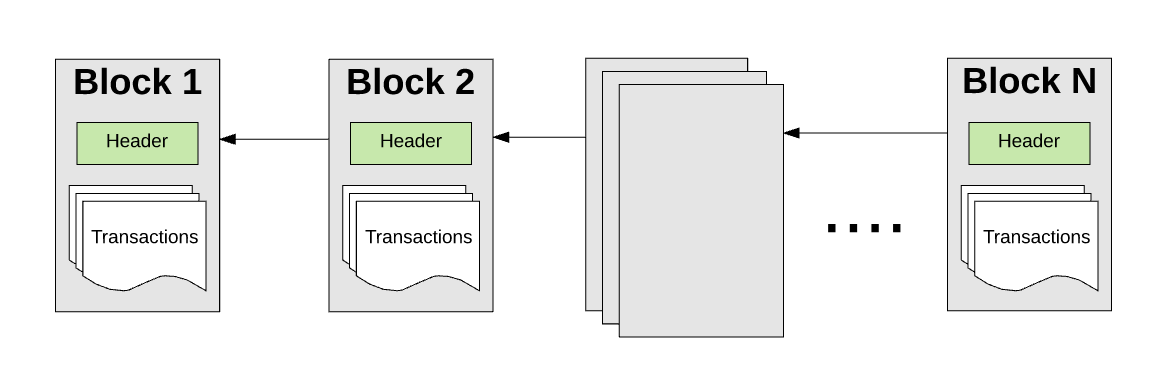
\includegraphics[width=\textwidth]{images/chain_of_blocks.png}
    \caption{Representation of a chain of blocks \cite{Medium}}
    \label{images:chain_of_blocks}
\end{figure}

Blocks are composed by an header and a body. The body simply contains the list of transactions associated with the block; the 
header instead contains general informations such as the hash of the current and of the previous block (in order to build a 
chain), the Merkle root that is an hash of the root of the Merkle tree in which are organized the transactions.
Apart these fundamentals properties every blockchain implementation can add its own header fields: common fields are nonce, 
the version of the system, the number of transactions contained etc.

Transactions are the minimal unit of information handled in the blockchain systems. Simply put, a transaction describes a 
transfer of information from an address to another. Every block can contains some hundreds of transactions.


\section{Ethereum}
\label{blockchain:ethereum}
All features and benefits described until now are common to all blockchain platforms but every product can 
add its own implementation over that or customize some behaviours.

One of the most famous and interesting platform available on the market today is \textbf{Ethereum}. It's 
an open source project, this means that everyone can contribute in his development and download its source 
code to understand in detail how it works.
\begin{figure}[!ht]
    \centering

\includegraphics[width=105mm]{images/ethereum.jpg}
    \caption{Ethereum project icon}
    \label{images:ethereum}
\end{figure}
Ethereum has a main peculiarity compared to its competitors: it was designed to be flexible and to adapt to 
different contexts, to be general-purpose.
In order to achive these objectives it is based on the \textbf{Ethereum Virtual Machine} (EVM) that is 
the ``runtime" of this platform. EVM is ``Turing complete", this means that it can execute code of arbitrary 
algorithmic complexity. Every node connected on the blockchain execute its own EVM allowing for the 
maintenance of the consensus over the network, even if has a huge computational cost and makes the entire 
system slower.

The foundamental task of the EVM is to execute \textbf{Smart Contracts}.
Just the smart contracts are the tools that allow Ethereum to be so flexible and generalized. Practically 
they are pieces of code that can do virtually everything, they reside on the blockchain and are loaded 
from users. This means that every user with a minimal programming background can partialy lead Ethereum 
behaviour.

The concept of ``Smart Contract" implicitly introduces the notion of \textbf{DAPP}: the DAPPs are common applications (web 
sites, mobile or desktop applications or also IoT apps) that uses as server the blockchain through the usage of a Smart 
Contract. In practice smart contracts are a middleware used to store data or execute actions on Ethereum. Actually there are 
a lot of DAPP in production on Ethereum and other in development but with some active users; they are about the most disparate 
business areas: there are a lot of games, a lot of cryptocurrencies and of exchanges, then some identity managers or food 
traceability. Figure \ref{images:solution_architecture} shows an example of an architecture of a system based on Ethereum.

\begin{figure}[!ht]
    \centering
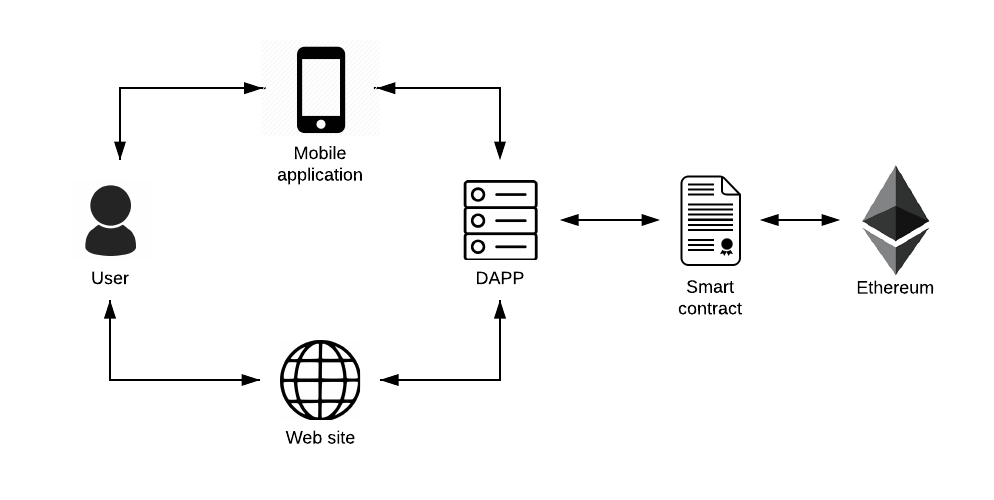
\includegraphics[width=\textwidth]{images/solution_architecture.png}
    \caption{Example of a solution architecture}
    \label{images:solution_architecture}
\end{figure}

Every operation executed by the EVM (storage of information, contract execution and so on) has a cost: for every transaction 
users must pay a small fees to the network. This payment has two main advantages: it prevents malicious computational tasks 
(DDoS attacks) and encourages people to mine Ethereum. The mining is the process of receive, propagate, verify, execute 
transactions and group them in blocks. These tasks are complex and really expensive from the computational point of view for 
this powerfull hardware and good electrical system are needed to do that. Miners are rewared for each block they mine with 
\textbf{Ether} (ETH), Ethereum’s native value-token.

Addresses in Ethereum are called \textbf{Accounts} and there are two kind of them: Externally Owned Accounts (EOAs) that are 
accounts handled by a person or an organization of the real world and Smart Contracts.

Ethereum transactions, over the fields common to all blockchain technologies, have a set of peculiar properties. Figure 
\ref{images:transactions_structure} is a screenshot taken from Etherscan (\ref{blockchain:ethereum_tools}) and shows the 
structure of a transaction in Ethereum. It has these properties:

\begin{itemize}
    \item \textbf{TxHash}, is the hash of the transaction, a way to uniquely identify it
    \item \textbf{Block Height}, is a reference to the block that contains the transaction (using its index)
    \item \textbf{Timestamp}, indicates when the transaction has been added to the blockchain
    \item \textbf{From}, represents the address from which the transaction start (the sender)
    \item \textbf{To}, is the address to which the transaction arrive (the receiver)
    \item \textbf{Value}, reveals the amount of Ether exchanged in the transaction
    \item \textbf{Gas limit}, shows the limit of gas that can be spend in a single transaction
    \item \textbf{Gas Used By Transaction}, defines the effectively used amount of gas (less then or equal to Gas Limit)
    \item \textbf{Gas Price}, is the price of the single unit of gas
    \item \textbf{Actual Tx Cost/Fee}, indicates the cost of the mining of the transaction (Gas price * Gas used)
    \item \textbf{Nonce}, is a value that enable to satisfy the proof-of-work
\end{itemize}

In general apart from the presented fields there is another one in Ethereum transactions: the ``Input Data" used to pass 
parameters or, for contracts, to select which method to execute.

\begin{figure}[!ht]
    \centering
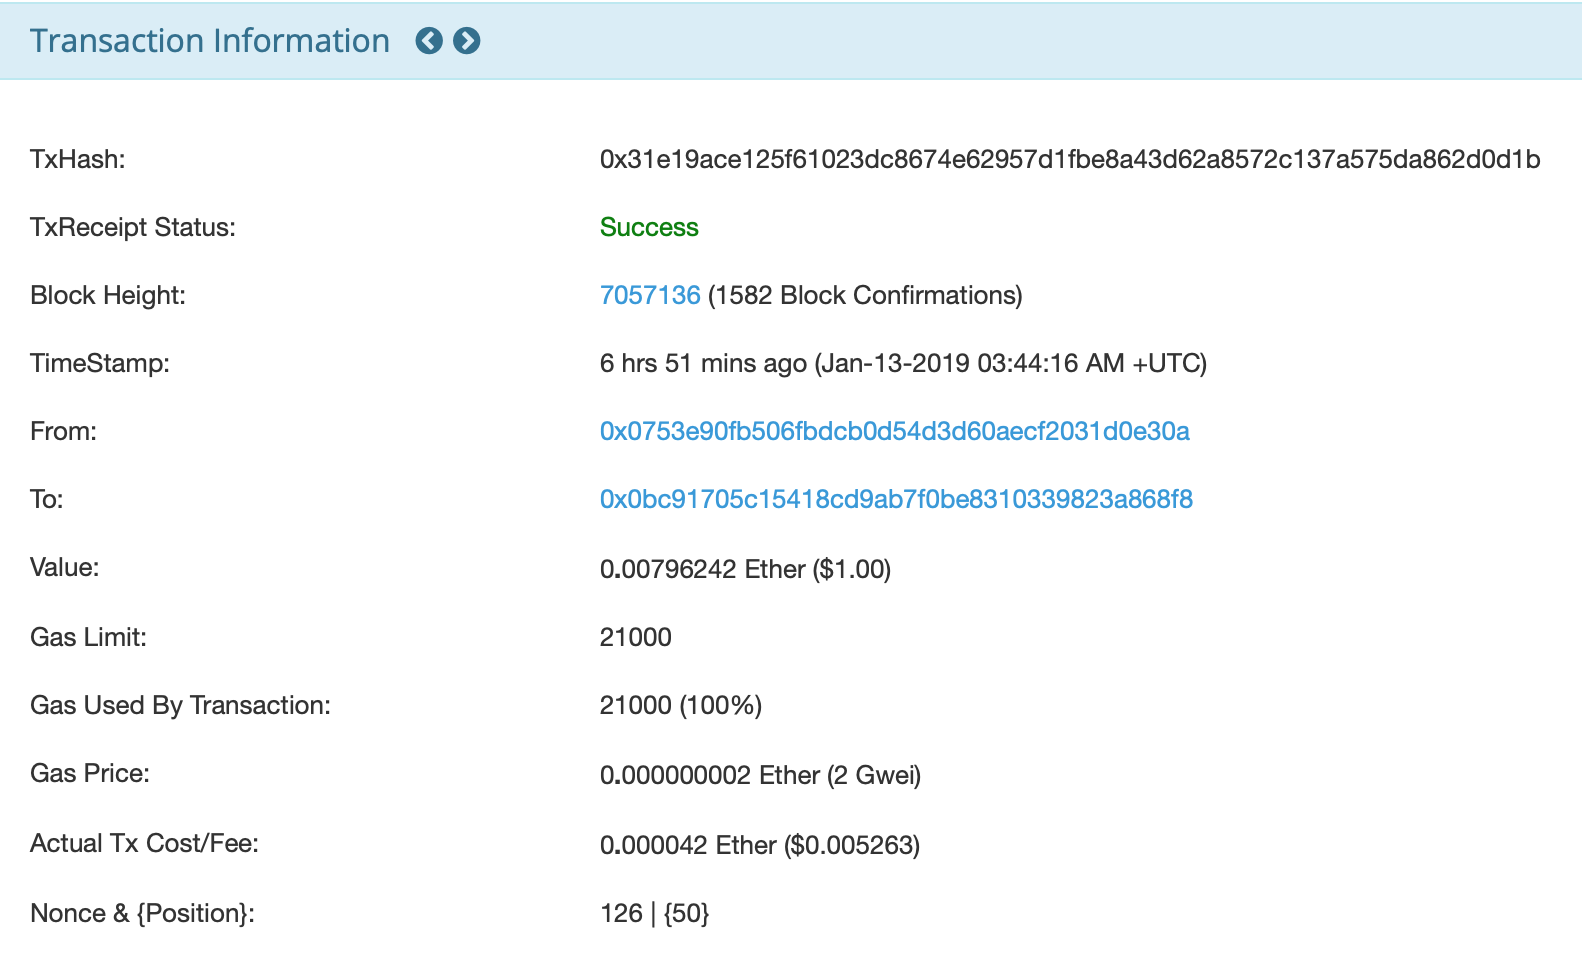
\includegraphics[width=\textwidth]{images/transactions_structure.png}
    \caption{Structure of an Ethereum transaction}
    \label{images:transactions_structure}
\end{figure}



\section{Ethereum tools}
\label{blockchain:ethereum_tools}
In order to work with Ethereum there are some tools needed and other that makes your life simpler.

\subsection{Clients}
Everyone can build its own Ethereum node with few simple steps: it is enough to install a client on a machine. There are a lot 
of official clients developed in various programming languages and that support almost all operating systems. Every client 
has its advantages and disadvantages even if all of them are pretty stable; the most used clients are \textbf{Parity}, 
\textbf{Go-Ethereum} and \textbf{Cpp-Ethereum}. After the installation these applications start the syncronization to the 
network: this is a costly operation that can take from various hours up to few days and will occupy some tens of GB on the 
machine disk. A local node can be referred in order to execute transactions, load contracts and interact in any other way with 
the blockchain.

\subsection{Explorers}
To read data from Ethereum there are different possible approaches: usually clients offer a UI and sometimes there are sections 
to explore data stored in the blockchain. Another chance consist in using the api exposed from the clients (RPC calls) to 
obtain row data. Anyway none of these two approaches are so comfortable: the first one allows to access only a subset of the 
data and the second one imply a certain technical competence. In general Explorer are used. Explorers are softwares that 
indexes all data on the blockchain in order to have a fast access to them. The most famous and used Etehreum explorer is 
Etherscan (https://etherscan.io). Etherscan allows the user to access all data on Ethereum in a very rapid way, its dataset is 
updated on the fly and shows some summary charts. Morover it expose some APIs for registered users that helps developers to 
get blockchain data in an aggregate form.

\subsection{Solidity}
Developers who wants to develop a Smart Contract should study \textbf{Solidy}. Solidity is a Contract-Oriented programming 
language influenced by C++, Python and JavaScript and is designed to target the EVM. Solidity is statically typed, supports 
inheritance, libraries and complex user-defined types among other features.

Listing \ref{listing:solidity} shows a very simple example of Smart Contract that allows users to store a numeric value on 
the blockchain.

\begin{lstlisting} [caption = {Simple solidity contract}, label = {listing:solidity}, language=Solidity]
    pragma solidity ^0.5.0;

    contract SimpleStorage {
        uint storedData;

        function set(uint x) public {
            storedData = x;
        }

        function get() public view returns (uint) {
            return storedData;
        }
    }
\end{lstlisting}

In general solidity supports classical value types such as boolean, integers and strings but it also supports a value type 
called ``address": it is a reference to an Ethereum address that can be used to Ether exchanges. All common  control-flow 
expressions are supported (if, else, while, return, etc.) Also visibility constructs are available: external, public, internal 
and private: every of them decide if a function or a property is available to the outside of the contract and/or to its 
internal.

Solidity supports multiple inheritance including polymorphism. When a contract inherits from other contracts, only a single 
contract is created on the blockchain, and the code from all the base contracts is compiled into the created contract. 
Another important tool for solidity developers are interfaces: they are similar to abstract contracts, but they cannot have 
any functions implemented. There are further restrictions:

\begin{itemize}
    \item They cannot inherit other contracts or interfaces.
    \item All declared functions must be external.
    \item They cannot declare a constructor.
    \item They cannot declare state variables.
\end{itemize}

Often interfaces are used to join to some standard as for example ERC20 tokens.


\subsection{Web3.js}
Last but not least tool introduced is Web3.js. This is a javascript library that exposes some incredibly simple apis that 
allow developers to interact with the blockchain. In practice this library interacts with a network node (local or remote, it 
does not matter) calling the RPC exposed from some client installed into the node address. 
Practically this library act as a gateway, hiding the complexity of an RPC call to the developer that simply invoke a 
javascript function. Then the client does his work and returns results to Web3.js which in its turn forward these results to 
the caller javascript application.

This library has a lot of features: it allows to reading the data on the blockchain, to register for Ethereum events (as for example 
new blocks or transactions), to invoke contracts and to manage personal informations and wallets.
\chapter{Process Mining}
\label{process_mining}

Objective of this chapter is to introduce some basic concepts about \textbf{Process Mining}, starting from Business Process 
Management, defining the concept of Process and finally presenting some tools available on the market. The purpose of this 
first part is to allow also to not expert readers to understand the work done in this thesis.

At a first place there is a little introduction in the world of \textbf{Business Process Management} in section 
\ref{process_mining:bpm} which helps to better understand the utility of process mining.
After that there is a general overview of process mining in section (\ref{process_mining:overview}) where are described some 
key notions of the theme: different kind of process mining, principles and standards.
Section \ref{process_mining:algorithms} focuses on process model discovery, illustrating the most used \textbf{algorithms} in 
this field.
Section \ref{process_mining:tools}, the last of the chapter, has the purpose of show the main software \textbf{tools} used to 
work with process mining.


\section{Business Process Management}
\label{process_mining:bpm}
BPM is the set of all activities to support and improve organisation performance by managing chains of events, tasks, and 
decisions that ultimately add value to the organisation. It includes concepts, methods, and techniques to support the design, 
administration, configuration, enactment, and analysis of business processes \cite{DBLP:books/WeskeBPM}.

A Business Process is described as “a collection of related and structured activities undertaken by one or more organisations 
in order to pursue some particular goal. Within an organisation a business process results in the provisioning of services or 
in the production of goods for internal or external stakeholders. Moreover business processes are often interrelated since 
the execution of a business process often results in the activation of related business processes within the same or other 
organisations” \cite{DBLP:journals/infsof/LindsayDL03}.

Around the notion of business process borns \textbf{Business Process Management}. As described in 
\cite{DBLP:books/sp/DumasRMR18} Business Process Management (BPM) is the set of activities needed to define, optimize, monitor 
and integrate business processes in order to make effective company's business. In \cite{DBLP:books/WeskeBPM} is described the 
BPM \textbf{``lifecyle''} shown in the Figure \ref{images:bpm_lifecycle}.

\begin{figure}[!ht]
    \centering
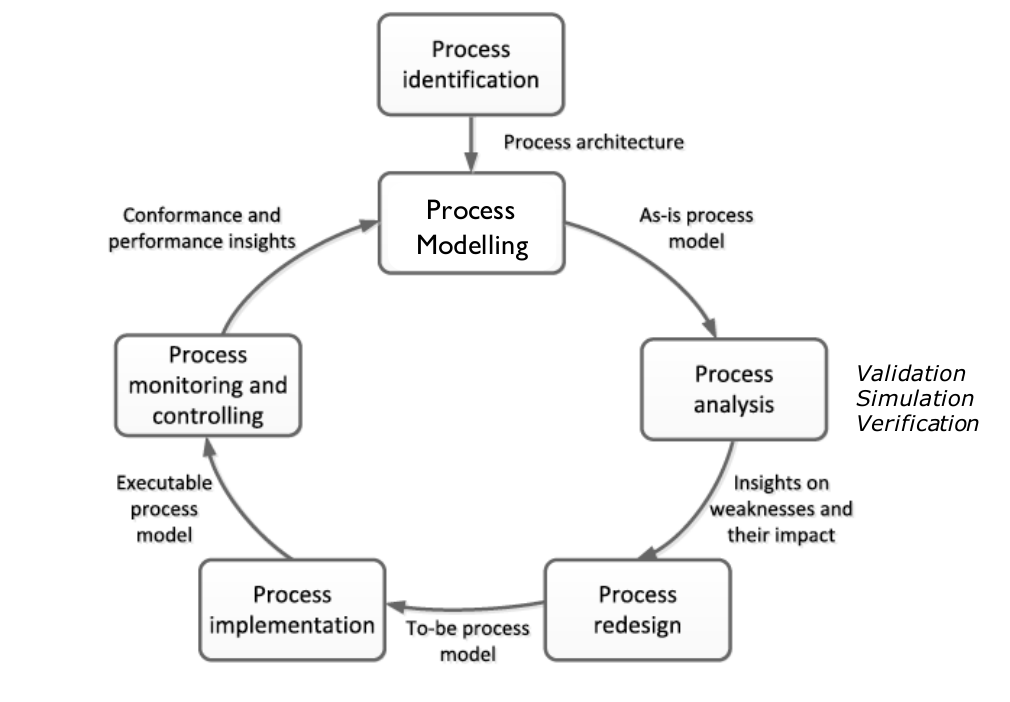
\includegraphics[width=\textwidth]{images/bpm_lifecycle.png}
    \caption{Business Process Management lifecycle \cite{DBLP:books/sp/DumasRMR18}}
    \label{images:bpm_lifecycle}
\end{figure}

We can see that there are 6 phases in the BPM lifecycle and that 5 of them are in a cycle: this means that these can 
be executed many times in order to continually refine the business processes. Let's describe shortly the different 
phasis:

\begin{itemize}
    \item \textbf{Process identification}: this step is executed only one time when the company start to model its 
        processes (for each process that must be deal with).

    \item \textbf{Process modeling}: this stage consists in the building of a process model that describe the real 
        life process. This activity is based on interviews with customer and industry experts and produce a model 
        of how the process is actually performed (as-is process model).

    \item \textbf{Process analysis}: at this level the ``as-is process model" is validated and design issues are
        identificated (this validation has 3 steps: validation, simulation and verification). A the end of this 
        phase there is a report of the model's weaknesses.

    \item \textbf{Process redesign}: if in the previous step some critical weakness were found, in this stage they 
        must be removed building the ``to-be process model".

    \item \textbf{Process implementation}: this phase has the goal of transform the to-be process model in a set 
        of rules that to be applied in order to change the current process execution. This set of rules is called 
        ``executable process model".

    \item \textbf{Process monitoring and controlling}: the last step of the lifecycle is the monitoring of the 
        changes applied to the process: in this task metrics are measured to understand how well the process 
        is performing. Is in this phase that process mining comes in to help to understand if there are some 
        problems and to improve process performance.
    
\end{itemize}


\section{Business Process Modelling Language}

The modeling step of the lifecycle needs some language to visualize and compare different process models: there are a lot of 
different notations but the most common is \textbf{Business Process Model and Notation} \cite{DBLP:journals/Chinosi} (BPMN) that is 
establishing itself as a de-facto standard. Another important and very used notation are \textbf{Petri Net}s (PN) 
\cite{PetriNetIntroduction}. They are pretty useful when there are verification needs.


\subsection{BPMN}
It was originally conceived and developed by the Business Process Management Initiative (BPMI). It is currently 
maintained by the Object Management Group (OMG). BPMN provides a notation that is simple and standard to make it 
understandable by people with different education and competence: management personnel, analysts and developers.

It maps 4 different types of objects: 

\begin{itemize}
    \item \textbf{Flow objects}, that can be events, activities or gateways. Events are represented as circle that can 
        contains other symbols to specify the type of the event. They can be Start, Intermediate or End events. Activities 
        are tasks that need to be done (sometimes they can be subprocess). Gateways determine the flow of the process and 
        in general are used to split and join different process behaviours.
    \item \textbf{Connecting Objects}, that can be sequence that allows to build the process flow, message that are used to 
        show the exchange of messages between different actors, or association that is used to associate Artifact, data or 
        text to a Flow Object. 
    \item \textbf{Swimlanes}, pools or lanes, used to organize different acitvities and in general lanes are sub-part of pools
    \item \textbf{Artifacts}, files, documents, objects, annotations, and so on.
\end{itemize}

For this thesis work only simple and basic Flow objects have been used, those shown in figure \ref{images:bpmn_flow_obj}.

\begin{figure}[!ht]
    \centering
    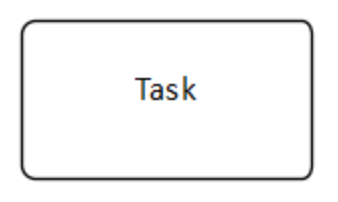
\includegraphics[width=30mm]{images/bpmn_task.png}
    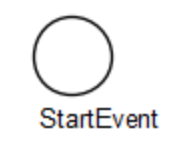
\includegraphics[width=20mm]{images/bpmn_start_event.png}
    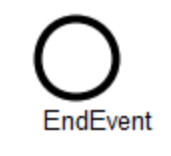
\includegraphics[width=18mm]{images/bpmn_end_event.png}
    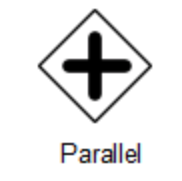
\includegraphics[width=16mm]{images/bpmn_parallel.png}
    
\includegraphics[width=18mm]{images/bpmn_exclusive.png}
    \caption{BPMN flow objects used in the thesis}
    \label{images:bpmn_flow_obj}
\end{figure}


\begin{figure}[!ht]
    \centering
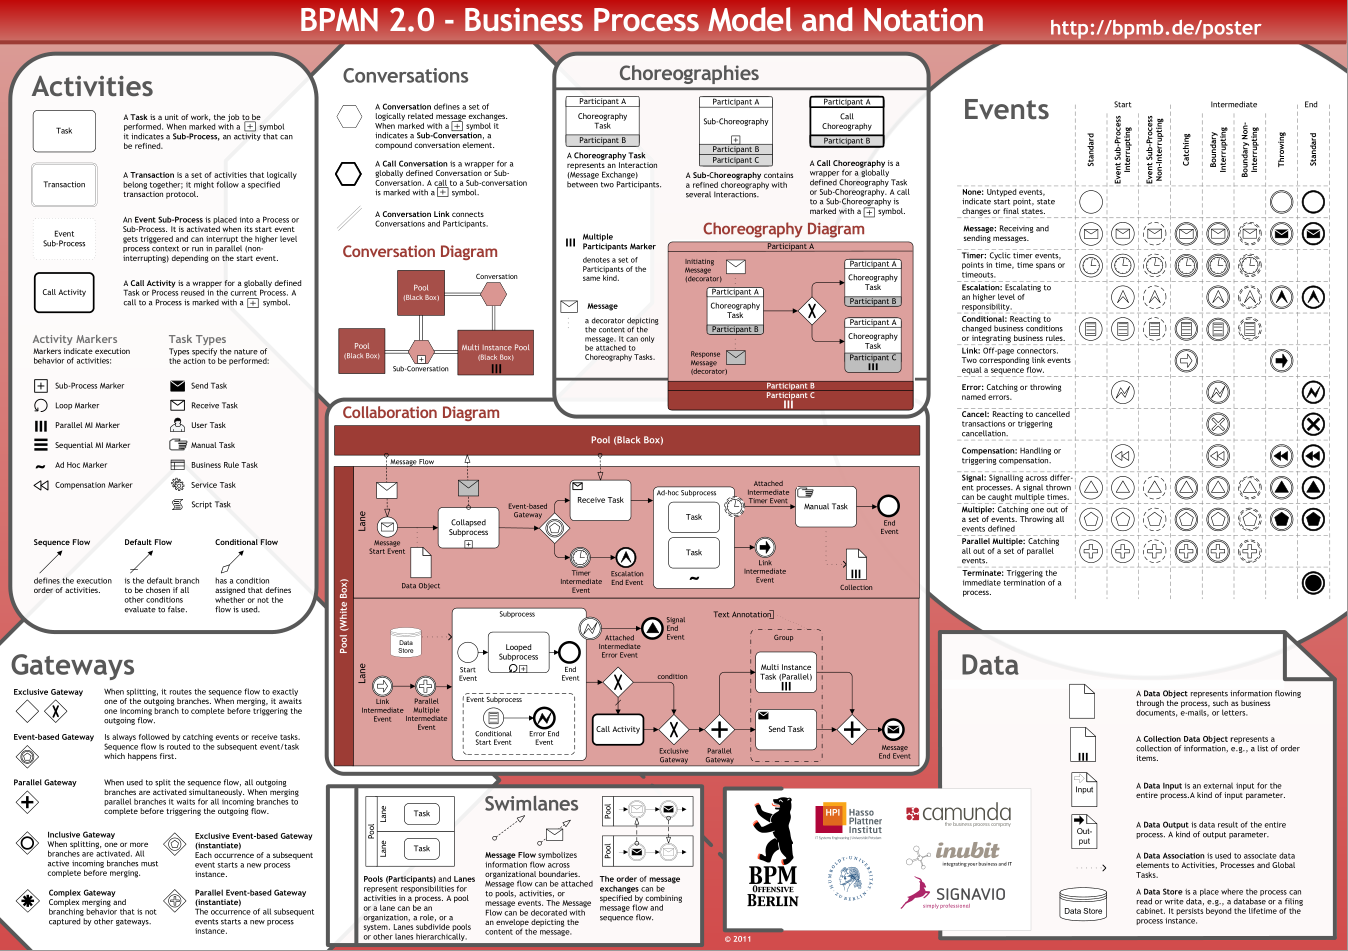
\includegraphics[width=\textwidth]{images/bpmn_manifesto.png}
    \caption{BPMN Manifesto}
    \label{images:bpmn_manifesto}
\end{figure}

BPMN allows the representation of interprocess communication or also process that include two or more stakeholders, it can 
be used for exceptions handling and other complex situations. For a complete set of BPMN elements see the Figure 
\ref{images:bpmn_manifesto}


\subsection{Petri Net}
Petri Nets are a really powerfull notation largely used in theoretical computer science in a big number of fields. They were 
formalized by Carl Adam Petri in its PhD thesis. They allow to model statics and dynamics systems throught a set of places, 
a set of transitions (or events) and a set of arcs that join places and transitions (Figure \ref{images:petri_net_elements} 
shows the representations of these elements). There are few and simple elements that allow for a huge power and flexibility. 
Dynamic systems can be described through the use of tokens that assumes different meanings based on the context: in BPM they 
are instances of the process. Tokens cross the net based to the ``fire rule": in practice a transiton can be crossed only if 
all its input places have the necessary number of tokens and in this case it generates the needed number of tokens for each 
of its output places.

\begin{figure}[!ht]
    \centering
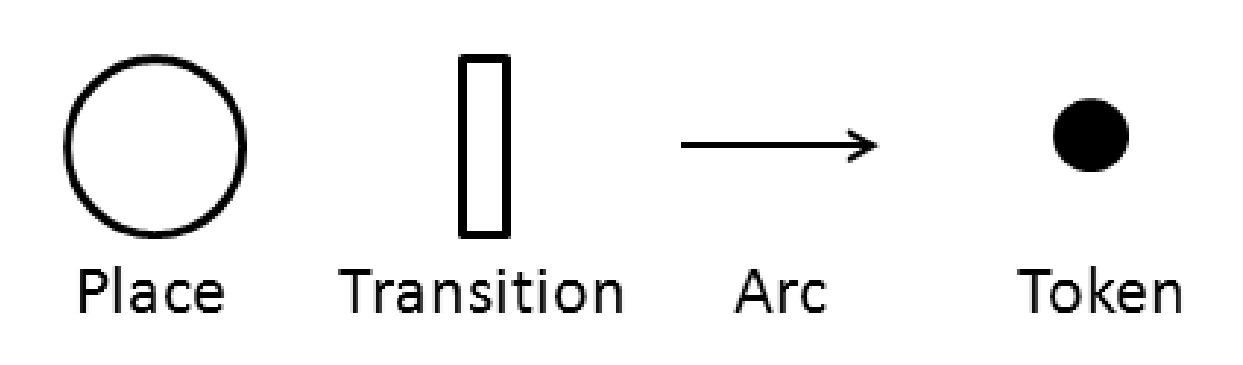
\includegraphics[width=70mm]{images/petri_net_elements.jpg}
    \caption{Petri net elements}
    \label{images:petri_net_elements}
\end{figure}

\section{Overview on Proess Mining Techniques}
\label{process_mining:overview}
The basic idea of the process mining is to infer, monitor and improve real life processes getting knowledge from 
software tool's logs.
Process mining includes the discovery of a process model (an automatic modeling) starting from the logs, the 
conformance checking between a logs and their discovered model, the individuation of relationship between people 
and the prediction of what will happens in a specific instance of a process.
process mining can be considered as a field that cross through Business Intelligence, Data Mining and Business 
Process Management.

\begin{figure}[!ht]
    \centering
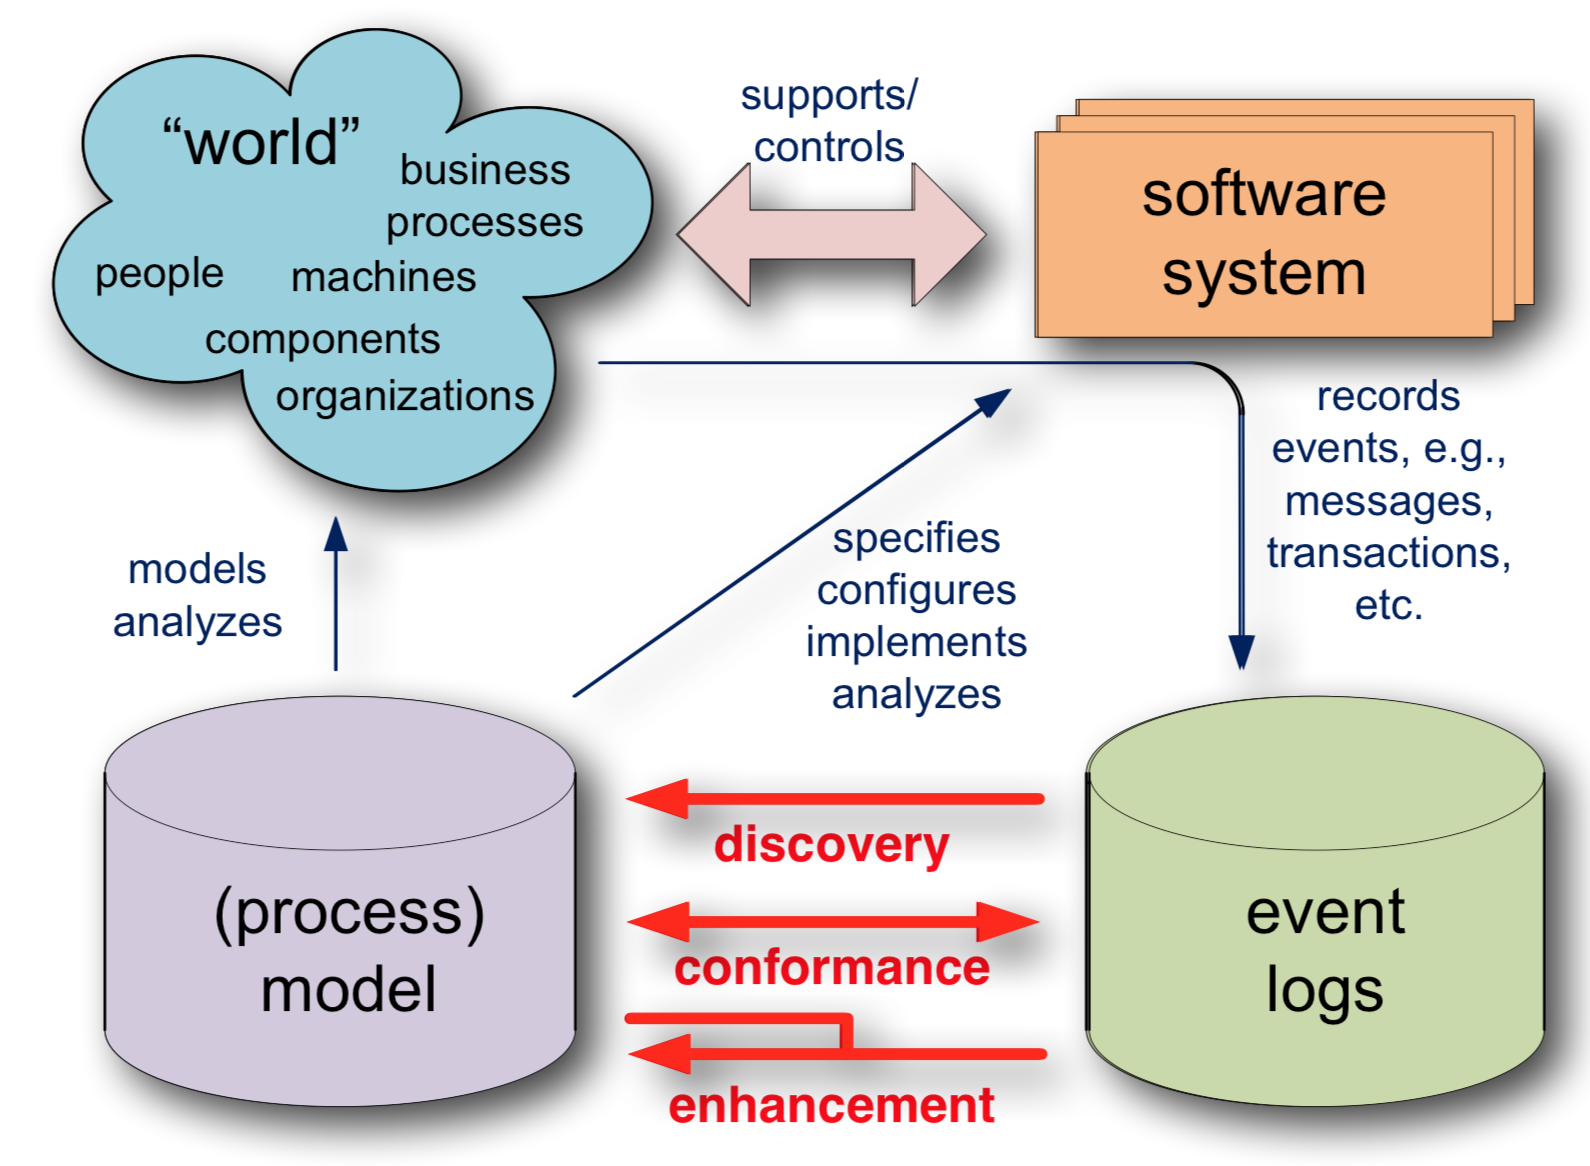
\includegraphics[width=\textwidth]{images/pm_resume.png}
    \caption{Schematic representation of process mining \cite{DBLP:conf/bpm/ProcessMiningManifesto}}
    \label{images:pm_resume}
\end{figure}

There are three forms of process mining:

\begin{itemize}

    \item \textbf{Process discovery}: these techniques allow to process a log, extract information from it and build a 
        process model with these information.

    \item \textbf{Conformance checking}: this type of process mining has the goal of evaluate the quality of a model: to 
        do so it compare the model with a log of the same process and measure how well they conform each other.

    \item \textbf{Enhancement}: in this case the idea is to extend or improve an existing process model using information 
        recorded on some event log.
    
\end{itemize}

\begin{figure}[!ht]
    \centering
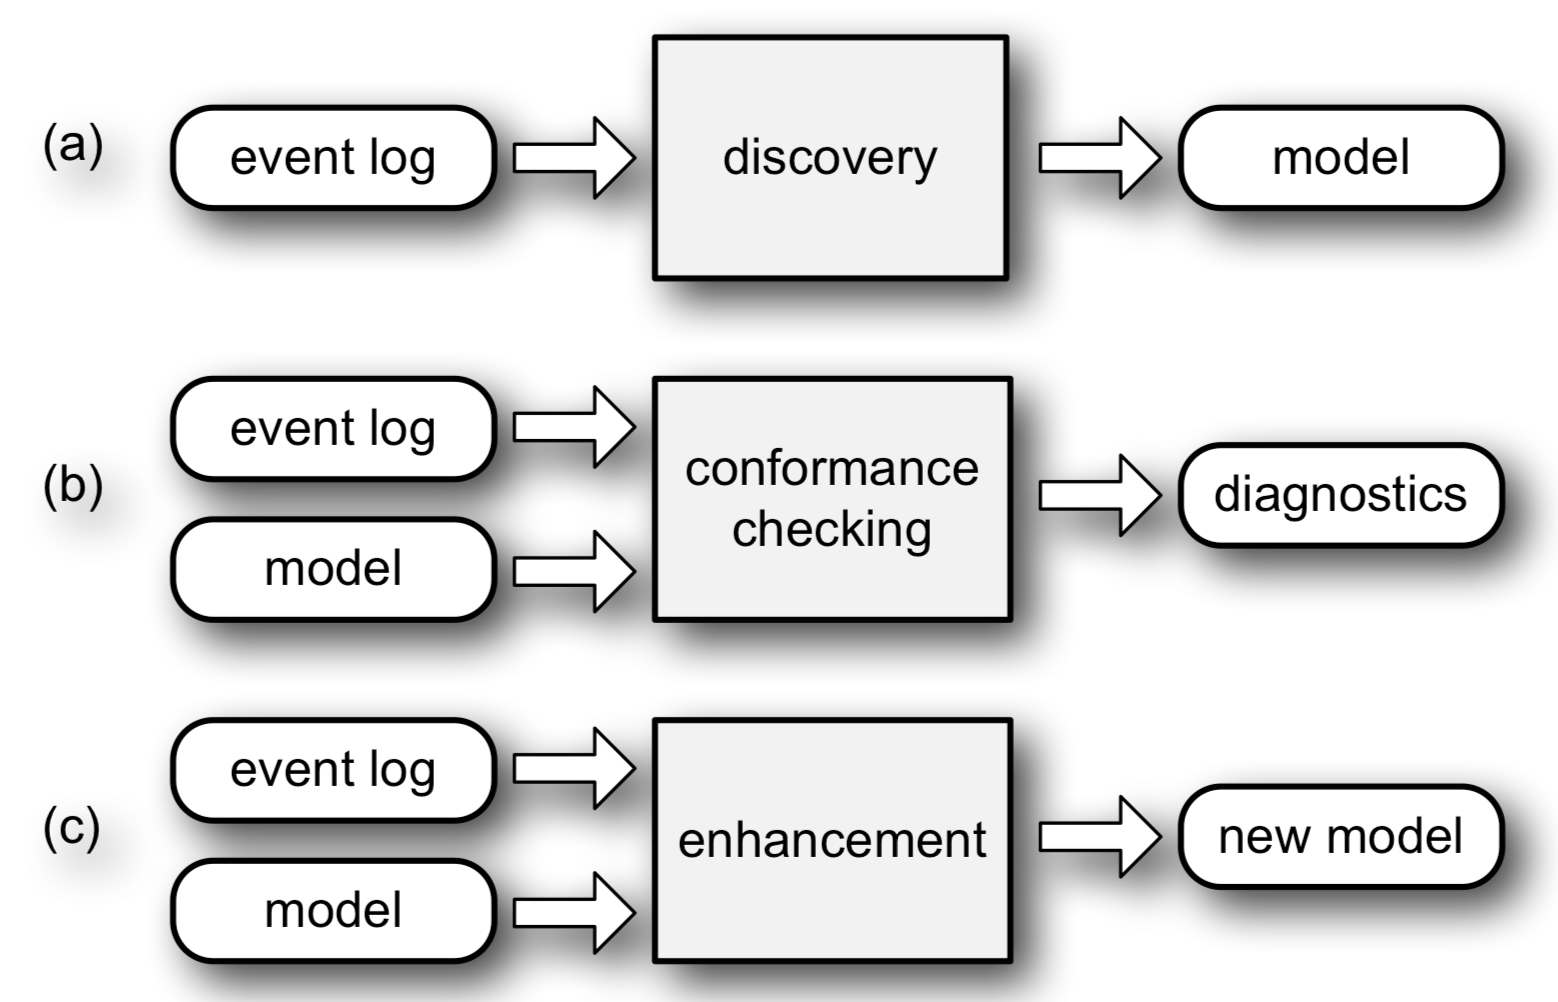
\includegraphics[width=\textwidth]{images/pm_io.png}
    \caption{Different process mining types input/output \cite{DBLP:conf/bpm/ProcessMiningManifesto}}
    \label{images:pm_io}
\end{figure}

It is important to specify that process mining is not limited to offline analysis even if is based on historical event data, 
infact it can be used even for running cases. For example it can be used to predict the completion time of a process instance 
or the choices a user will take in certain conditions, etc.

Process mining is a valuable methodology for most of the phases shown in Figure \ref{images:bpm_lifecycle}.

In Figure \ref{images:pm_project} are shown all steps of a process mining project.
First of all there is a planning activity and a justification for this planning. The second step consist in the extraction 
of all the interisting information needed in the project, current data available, and a good understanding of the domain. 
The result of this activity is a set of artifacts such as historical data, handmade models and objectives.
The next stage is the building of a control-flow model through the use of automated process discovery techniques.
In step 3 control-flow model is extended with other perspectives (documents, time, and resources). The last stage is the 
use of the models created in previous steps for operational support (intervene, predict, and recommend running processes).
Last stages can only be reached if the process is sufficiently stable and structured.

\begin{figure}[!ht]
    \centering
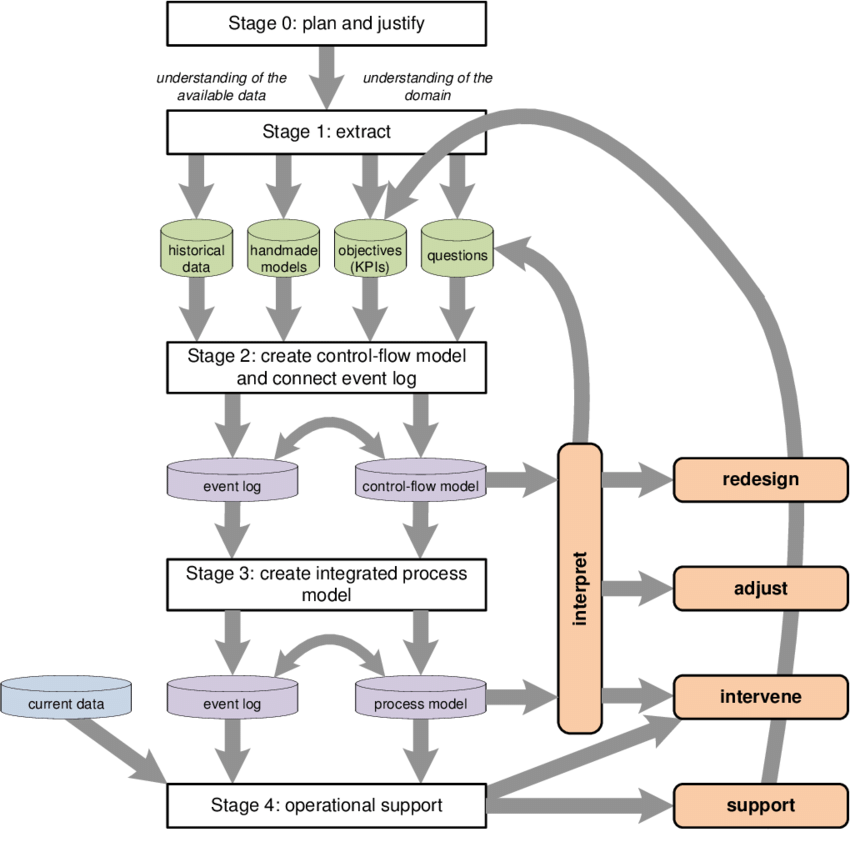
\includegraphics[width=\textwidth]{images/pm_project.png}
    \caption{Steps in a process mining project \cite{DBLP:conf/bpm/ProcessMiningManifesto}}
    \label{images:pm_project}
\end{figure}

As seen before logs are a central concept in process mining but until now the quality of the logs have not been considered 
even if the value of the results of a process mining activity mostly depends by the input. This means that with a poor or not 
precise log we will have not good results.
In Process Mining Manifesto there are a classification of the log value in 5 levels shown in Figure \ref{images:pm_loglevels}.

\begin{figure}[!ht]
    \centering
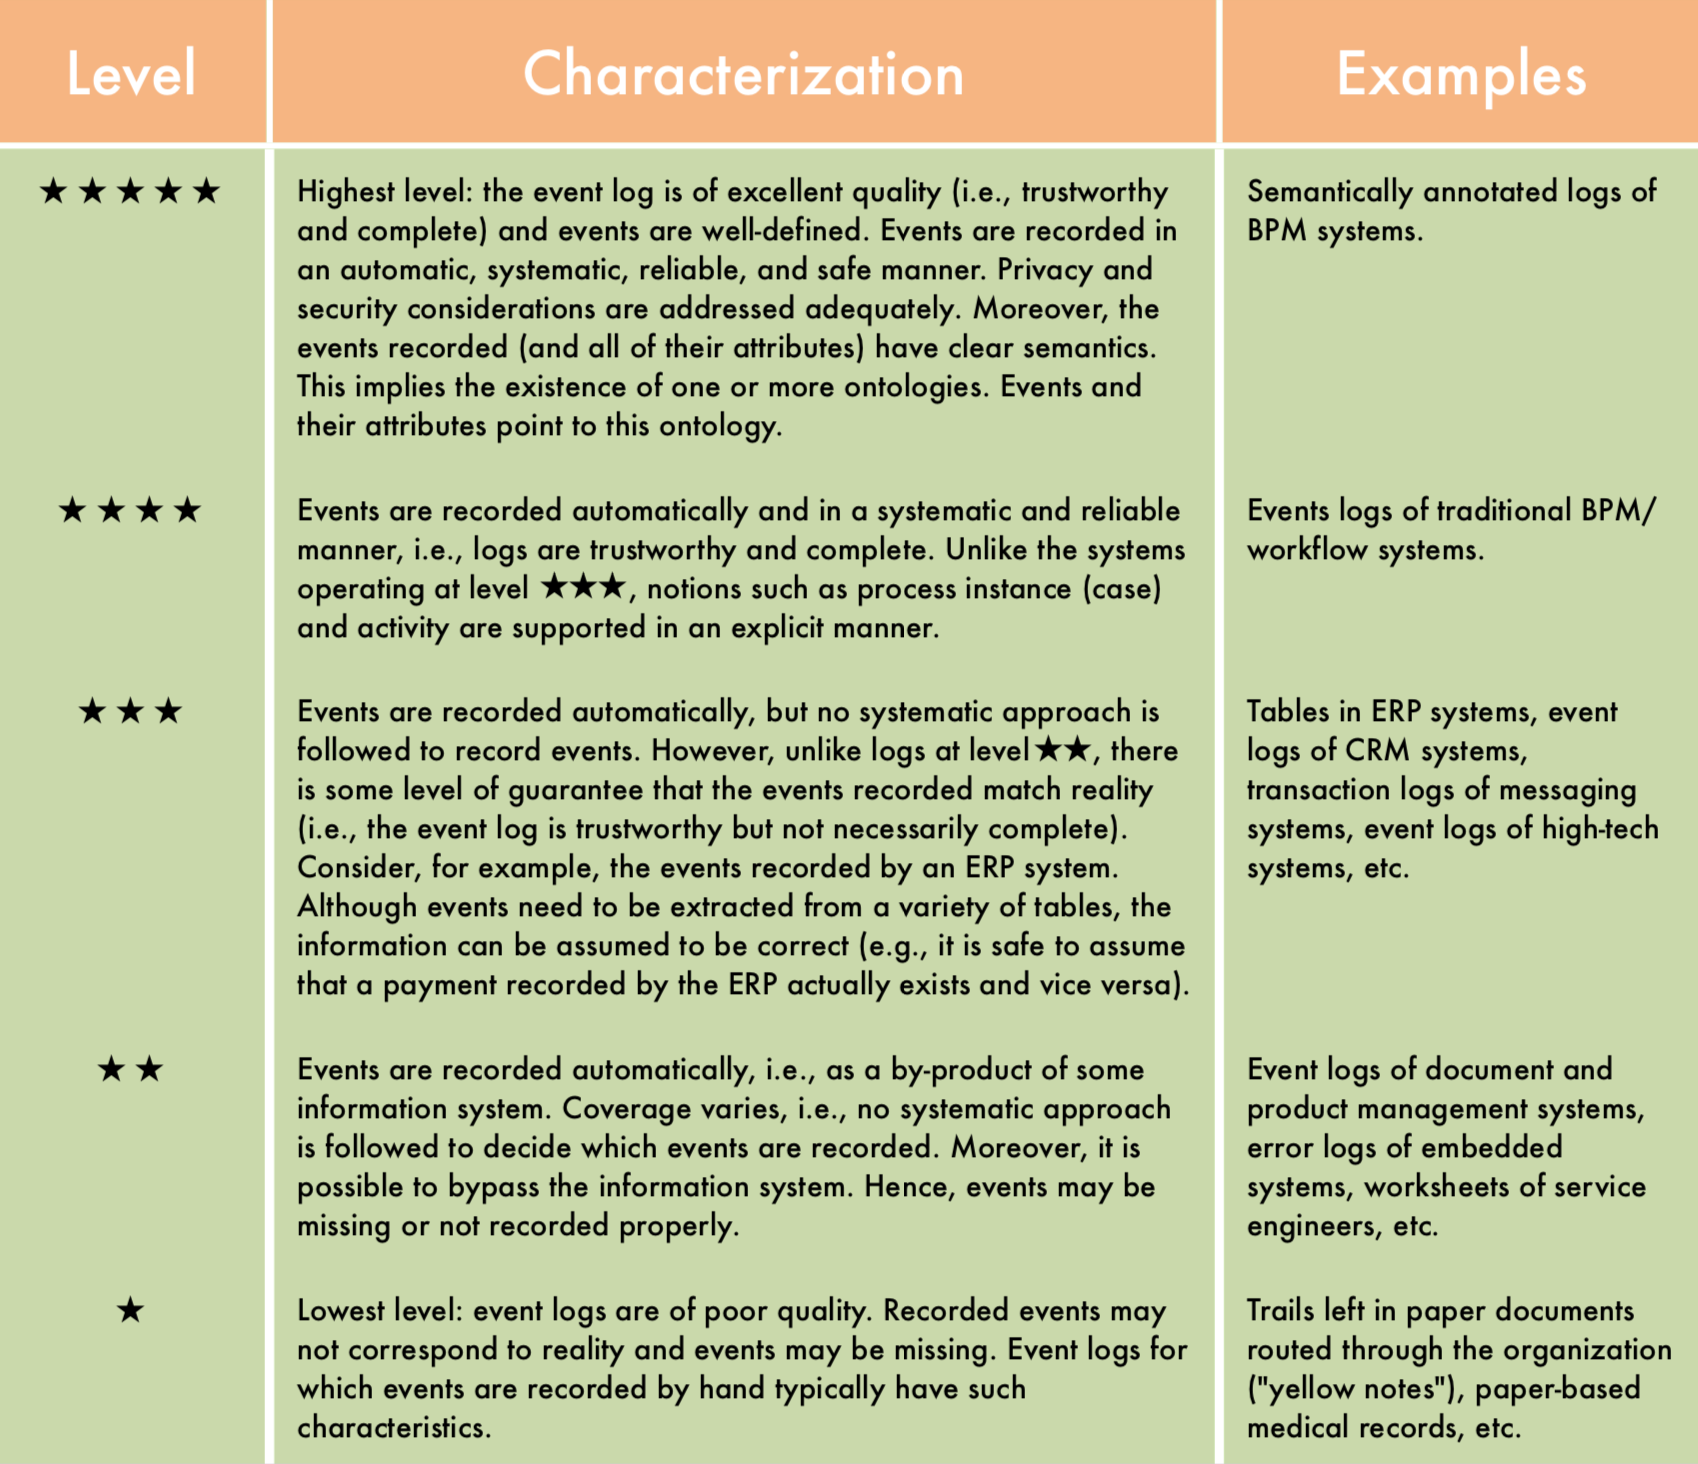
\includegraphics[width=\textwidth]{images/pm_loglevels.png}
    \caption{Maturity levels for event logs \cite{DBLP:conf/bpm/ProcessMiningManifesto}}
    \label{images:pm_loglevels}
\end{figure}

The last important thing to explain about logs is how they are formalized: in the available tools different formats are 
supported (csv, xls, etc.) but in the years a specific format for event logs was developed. \textbf{XES} (Extensible Event 
Stream) is an XML-based standard with the purpose to provide a generally-acknowledged format for the interchange of event 
log data between tools and application domains \cite{XESstandard}.
When designing the XES standard, the following goals have been used as guiding principles:
\begin{itemize}
    \item \textbf{Simplicity}, XES logs should be easy to parse and to generate, and they should be equally well 
        human-readable.
    \item \textbf{Flexibility}, the XES standard should be able to capture event logs from any background, no matter what 
        the application domain or IT support of the observed process. 
    \item \textbf{Extensibility}, it must be easy to add new constructs to the standard in the future while maintaining 
        backward and forward compatibility.
    \item \textbf{Expressivity}, all information elements must be strongly typed, and there must be a generic method to 
        attach human-interpretable semantics to them.
\end{itemize}

Example of XES standard in listing \ref{listing:xes}.

\begin{lstlisting} [caption = {Part of a trace in a XES file}, label = {listing:xes}]
<trace>
    <string key="concept:name" value="Case3.0"/>
    <event>
        <string key="concept:name" value="A"/>
        <int key="concept:instance" value = "1"/>
        <string key="org:resource" value="UNDEFINED"/>
        <date key="time:timestamp" value="2008-12-09"/>
        <string key="lifecycle:transition" value="complete"/>
    </event>
</trace>
\end{lstlisting}


The last important aspect to cover talking about Process Mining is the measure of the results that are being obtained: in this 
context the paper \cite{DBLP:conf/ReplayQualityParameters} introduce four parameters that allow to measure the quality of a discovered 
model in comparison to the event log that generated it: 

\begin{itemize}
    \item \textbf{Fitness}: quantifies the extent to which the discovered model can accurately reproduce the cases recorded 
        in the log.

        \(Fitness = 1 - \frac{\textrm{cost for aligning model and event log}}{\textrm{Minimal cost to align arbitrary event log on model and vice versa}}\)

    \item \textbf{Precision}: this value measures the level of underfitting, i.e. a poor precision means that a model admits 
        unusual behaviors than those shown in the logs.

        \(Precision = 1 - \frac
            {\sum_{\textrm{visited markings}} \#visits * \frac{\textrm{\#outgoing edges} - \textrm{\#used edges}}{\textrm{\#outgoing edges}}}
            {\textrm{\#total marking visits over all markings}
        }\)
        
    \item \textbf{Generalization}: is a measure of the model overfitting: an high level of generalization means that the model 
        can handle behaviors not seen in the log, maybe because not yet observed.

        \(Generalization = 1 - \frac
        {\sum_{\textrm{nodes}} \sqrt{\#executions}^{-1}}
        {\textrm{\#nodes in tree}}
        \)
        
    \item \textbf{Simplicity}: this param try to define a level of human readability of the process model.
    
        \(Simplicity = 1 - \frac{\textrm{\#duplicate activities} + \textrm{\#missing activities}}{\textrm{\#nodes in process tree} + \textrm{\#event classes in event log}}\)
        
\end{itemize}

\begin{figure}[!ht]
    \centering
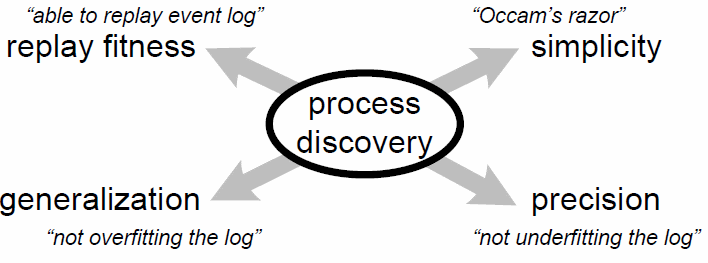
\includegraphics[width=80mm]{images/model_quality.png}
    \caption{Fitness, precision, generalization and simplicity \cite{DBLP:conf/ReplayQualityParameters}}
    \label{images:model_quality}
\end{figure}

Fitness, precision and generalization are measured replaying the traces in the original event log on the discovered process 
model with the format of Petri Net. This is a simple but, potentially, very long task and if done manually is very error prone. 


\section{Discovery algorithms}
\label{process_mining:algorithms}
This section start to focus on the discovery branch of process mining. In order to infer a model from an event log 
we can choose between different algorithms; there is not the best algorithm or the worst but for each case there is an 
algorithm that fits better the environment.

\subsection{Overview of the Alghoritms}

Here is a list of the most used algorithms: 

\begin{itemize}
    \item \textbf{Alpha Miner} 
    is one of the most precise algorithms. It builds a Petri Net generating a table of relationship between all events 
    (causality, parallel or nothing). It is very used in literature beacuse it is relatively simple to implement but it has 
    some known limitations: for example it cannot model loops of length 1 or 2. In order to remove this gap there are two 
    versions of the algorithm: rispectively Alpha+ and Alpha++.
    
    \item \textbf{Fodina}
    is a discovery method based on Heuristic Miner but more reliable when the event log is very noisy. Thanks to this 
    capability it can also handle the discovery based on user inputs. Its properties are discussed in \cite{DBLP:journals/dss/Fodina}.
    
    \item \textbf{Inductive Visual Miner} is described in \cite{DBLP:conf/bpm/InductiveVisualMiner}.
    This is more a tool than an algorithm, in fact it builds a chain of tasks and shows the changes live in a visual 
    format. Events can be filtered to hide them from the model, then Inductive Miner is used to discover the process 
    model. Than is possible to highlight important events, enrich the model and finally to animate it; animate a model 
    means to show different instances of the process in action using tokens that pass through different model steps over 
    time.
    
    \item \textbf{ILP Miner} is presented in \cite{DBLP:journals/fuin/ILPMiner}.
    This algorithm is based on Integer Linear Programming (ILP) techniques (also defined Constraint Programming). ILP 
    miner guarantee a fitness of 1, that means, that the model generated includes all the possibile traces found in 
    the log. This can be a wonderfull feature but not always: in most real-life processes there is some noise in the log, 
    some extremly rare events that should be ingored in the model in order to obtain a result closer to the real-life 
    process. Over that the fact that all possible traces are modeled can bring to an highly unreadable petri net 
    because the number of elements can grow a lot.
    Another negative aspect of this algorithm is that its execution time is bigger than others because ILP problems need 
    a lot of calculation to be solved.
    
    \item \textbf{Fuzzy Miner} was introduced in \cite{DBLP:conf/bpm/DiscoFuzzyMiner} and it is the algorithm used in the software tool Disco 
    for the process discovery. The Fuzzy Miner was the first mining algorithm to introduce the “map metaphor” to process mining, 
    including advanced features like seamless process simplification and highlighting of frequent activities and paths. The 
    result is a set of interesting and reliable information easy to understand also domain experts that do not have any 
    experience on process mining.
    
\end{itemize}


\subsection{Best fitting algorithms}
This section introduce three discovery algorithms which are that used in the practical part of the thesis:

\begin{itemize}

    \item \textbf{Heuristic Miner}:
    as alpha miner also heuristic miner mine the control-flow perspective of a process model building a dependency graph 
    but in a different manner: in fact it uses frquences of events to build this table. For example more 
    frequently a task ``A" directly follows another task B, and the less frequently the opposite occurs, the higher the 
    probability that ``A" causally follows ``B". This allow for noise management because rare events connection can be 
    omitted from the model. The usual output of this algorithm is a Heuristic Net or a Petri Net. While Heuristics Miner has 
    been shown to achieve relatively good fitness and precision in the presence of noise, in \cite{DBLP:conf/icdm/SplitMiner} is explained 
    that it still outputs spaghetti-like and unsound process models when applied to large real-life event logs.

    \item \textbf{Inductive Miner}:
    this is one of the fews algorithms that guarantee the soundness of the process model inferred. It uses a divide-and-conquer 
    approach to discover process trees: It first creates a DFG, filters infrequent directly-follows dependencies, and identifies 
    cuts in the filtered DFG. A cut is a control-flow dependency along which the log can be bisected. The identification of cuts 
    is repeated recursively, starting from the most representative one until no more cuts are found. Once all cuts are 
    identified, the log is split into portions (one per pair of consecutive cuts) and a process tree is generated from each 
    portion.
    In order to divide the activities in log L IM searches for a characteristic division of activities into disjoint sets, a cut, 
    of the directly-follows graph. Each operator (×, →, ∧ or cycle) has a characteristic cut of the directly-follows graph. 
    If such a characteristic matches, IM selects the corresponding operator. Otherwise, a flower model, allowing for all 
    sequences of activities, is returned. Than IM recurses until the model is completely discovered.
    

    \item \textbf{Split Miner}: 
    starting from a log, Split Miner produces a BPMN model in five steps as shown in Figure \ref{images:split_miner_steps}.

    \begin{figure}[!ht]
        \centering
    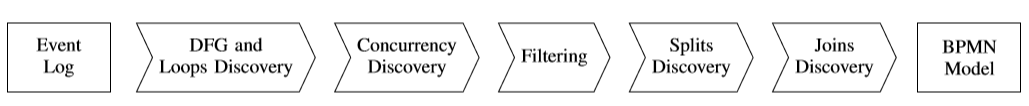
\includegraphics[width=\textwidth]{images/split_miner_steps.png}
        \caption{Split miner steps \cite{DBLP:conf/icdm/SplitMiner}}
        \label{images:split_miner_steps}
    \end{figure}

    Like the Heuristics Miner, the first step is to construct the DFG, but unlike the latter, Split Miner does not immediately 
    filter the DFG. Instead, it analyzes it to detect self-loops and short-loops and to discover concurrency relations 
    between pairs of tasks. Whenever a likely concurrency relation between a and b is discovered, the arcs between these two 
    tasks are pruned from the DFG. The result is called: pruned DFG (PDFG). In the third step, a filtering algorithm is 
    applied on the PDFG to strike balanced fitness and precision maintaining low control-flow complexity. In the fourth step, 
    split gateways are discovered for each task in the filtered PDFG with more than one outgoing arc. This is followed by the 
    discovery of join gateways that is the last step of the alghoritm.
    
\end{itemize}


\section{Tools}
\label{process_mining:tools}

Process mining is a relatively new area of research but it is enough mature to have a set of support tools that enable the 
application of its principles. These software tools implements some of algorithms listed in the previous section, using 
standards and offering a graphical approach.

\subsection{ProM}
ProM is an extensible framework, it is platform independent as it is implemented in Java, and can be downloaded free.
It supports a wide variety of process mining techniques in the form of plug-ins (this is why it is defined as extensible). 
ProM UI is organized in three subsections: \textbf{Object view}, \textbf{Action view} and \textbf{Visualization view}.

\begin{figure}[!ht]
    \centering
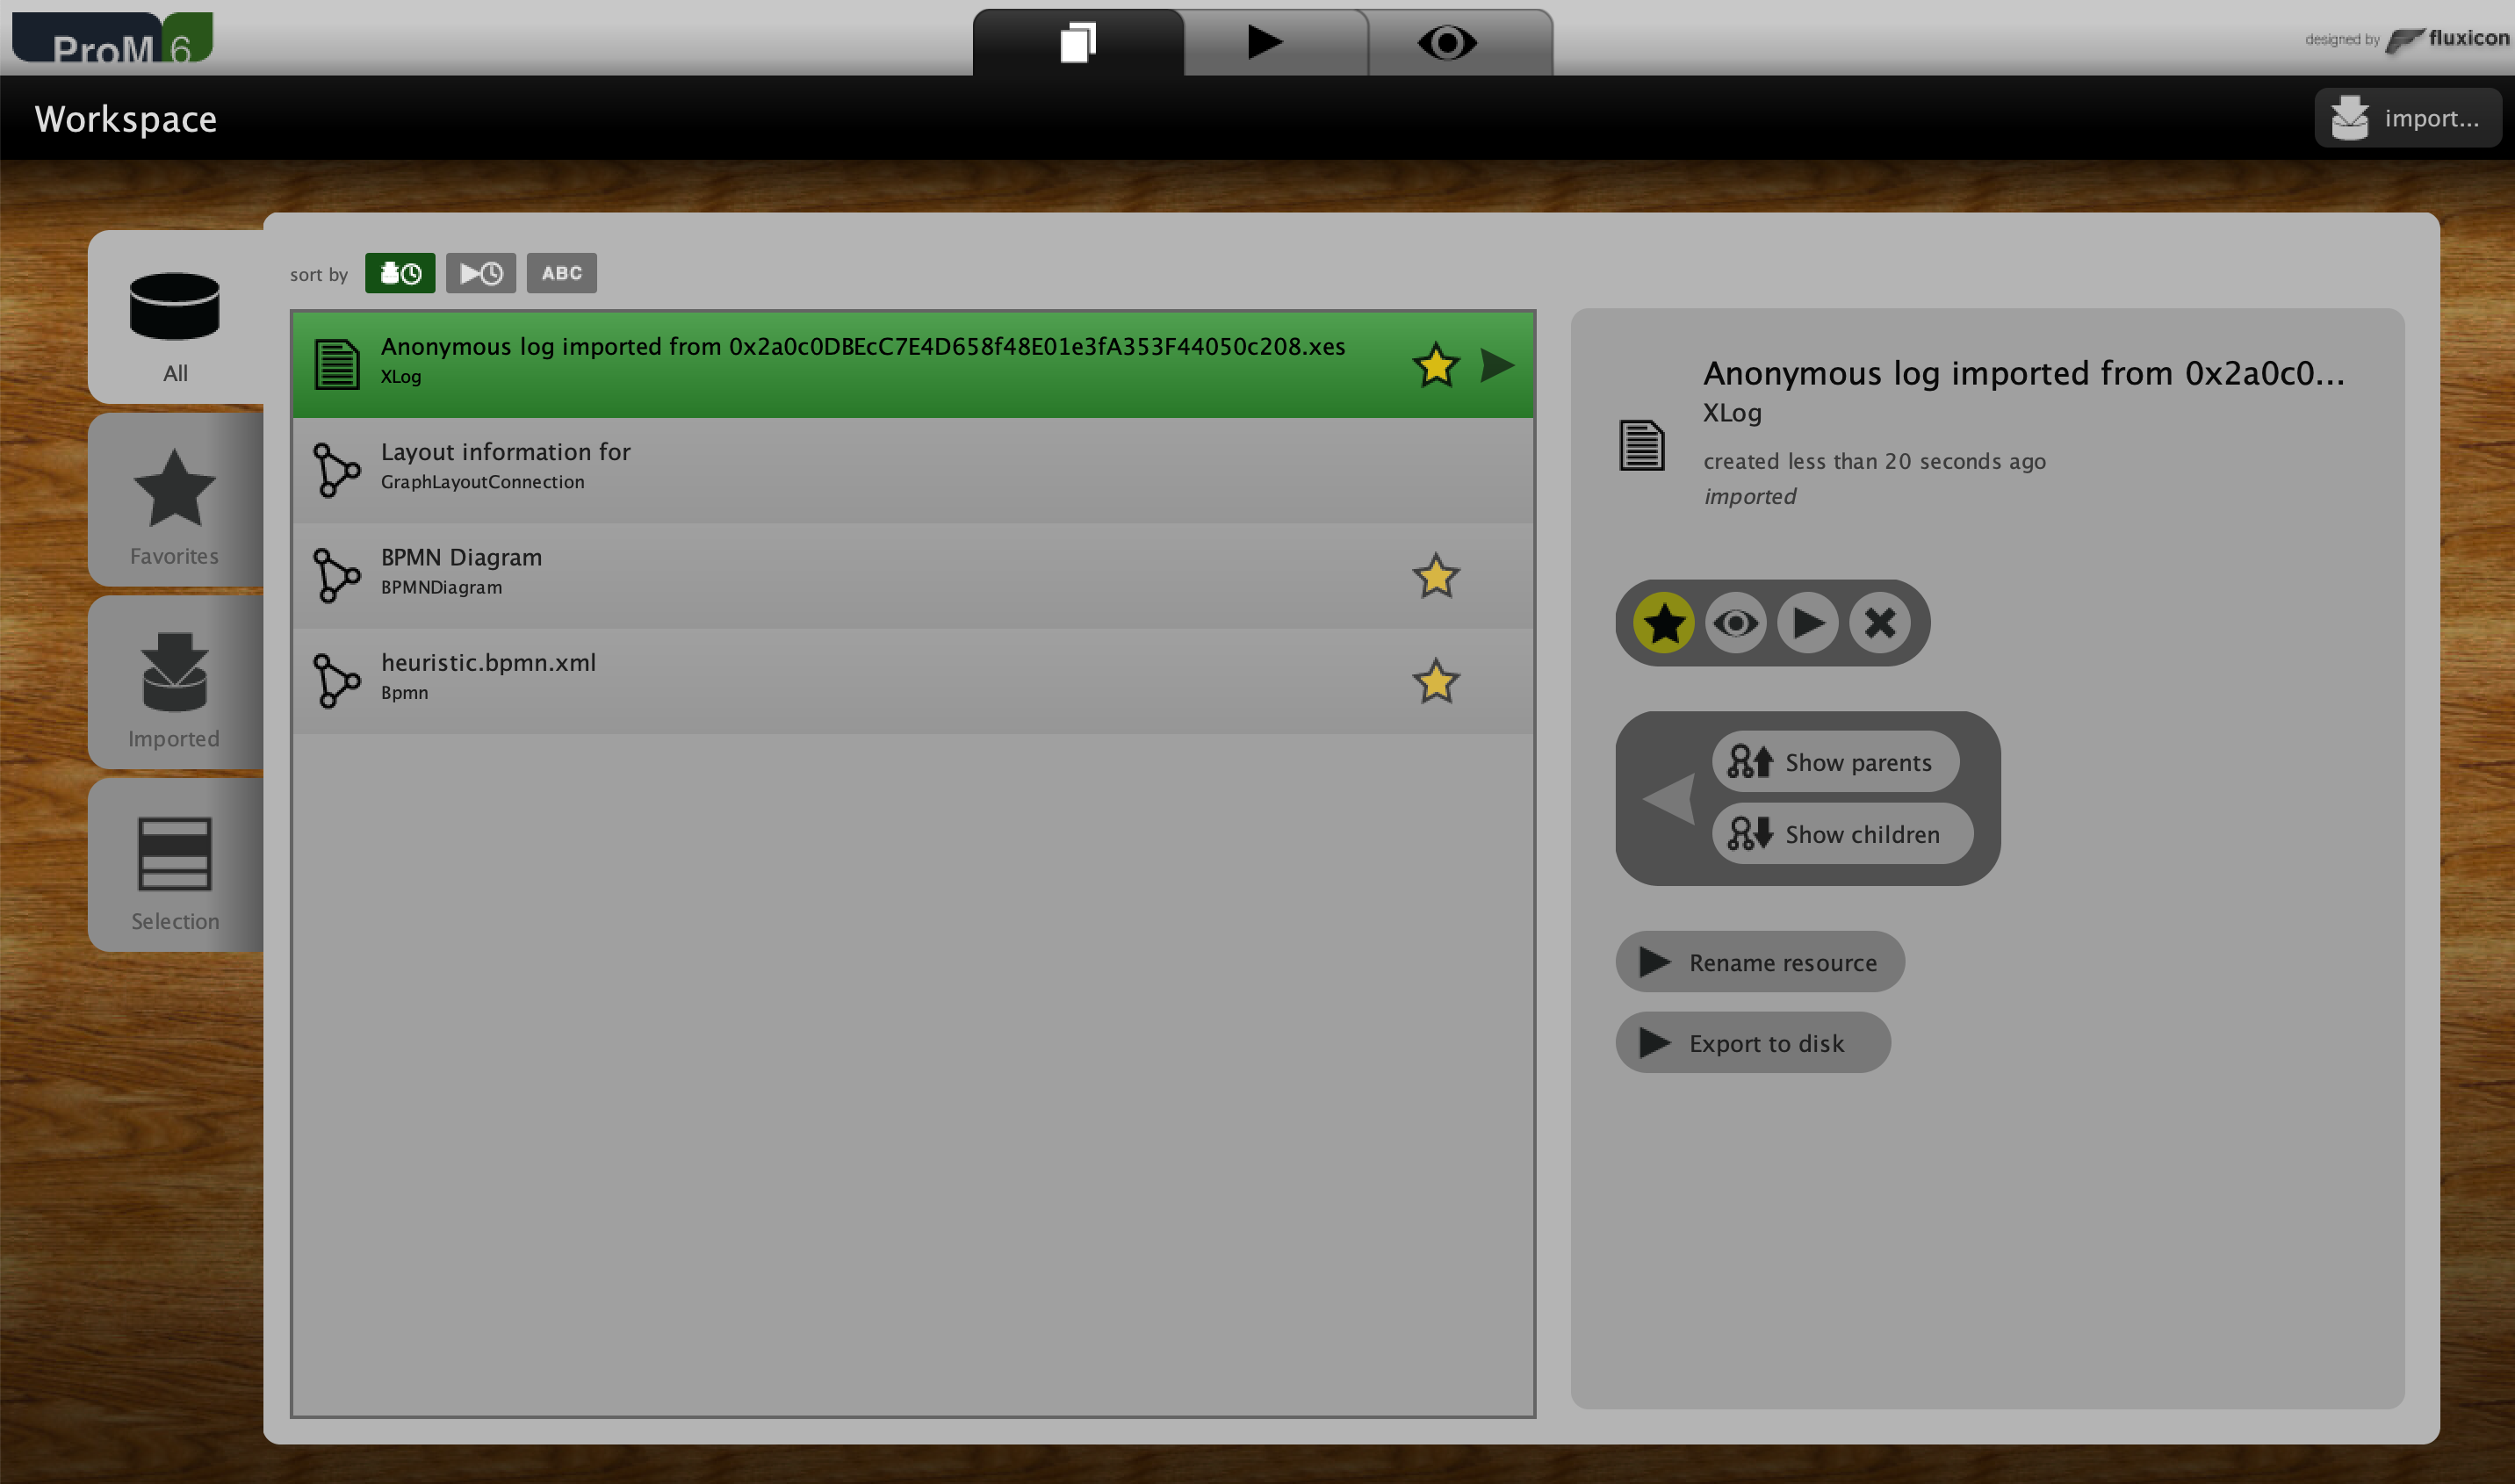
\includegraphics[width=\textwidth]{images/prom_screen_object.png}
    \caption{ProM object view screenshot}
    \label{images:prom_screen_object}
\end{figure}

In object view there are all objects you have work with: imported files, event logs, results of some ProM plugin, everything.
The visualization section renders objects in different ways: process trees, petri nets, images etc.

\begin{figure}[!ht]
    \centering
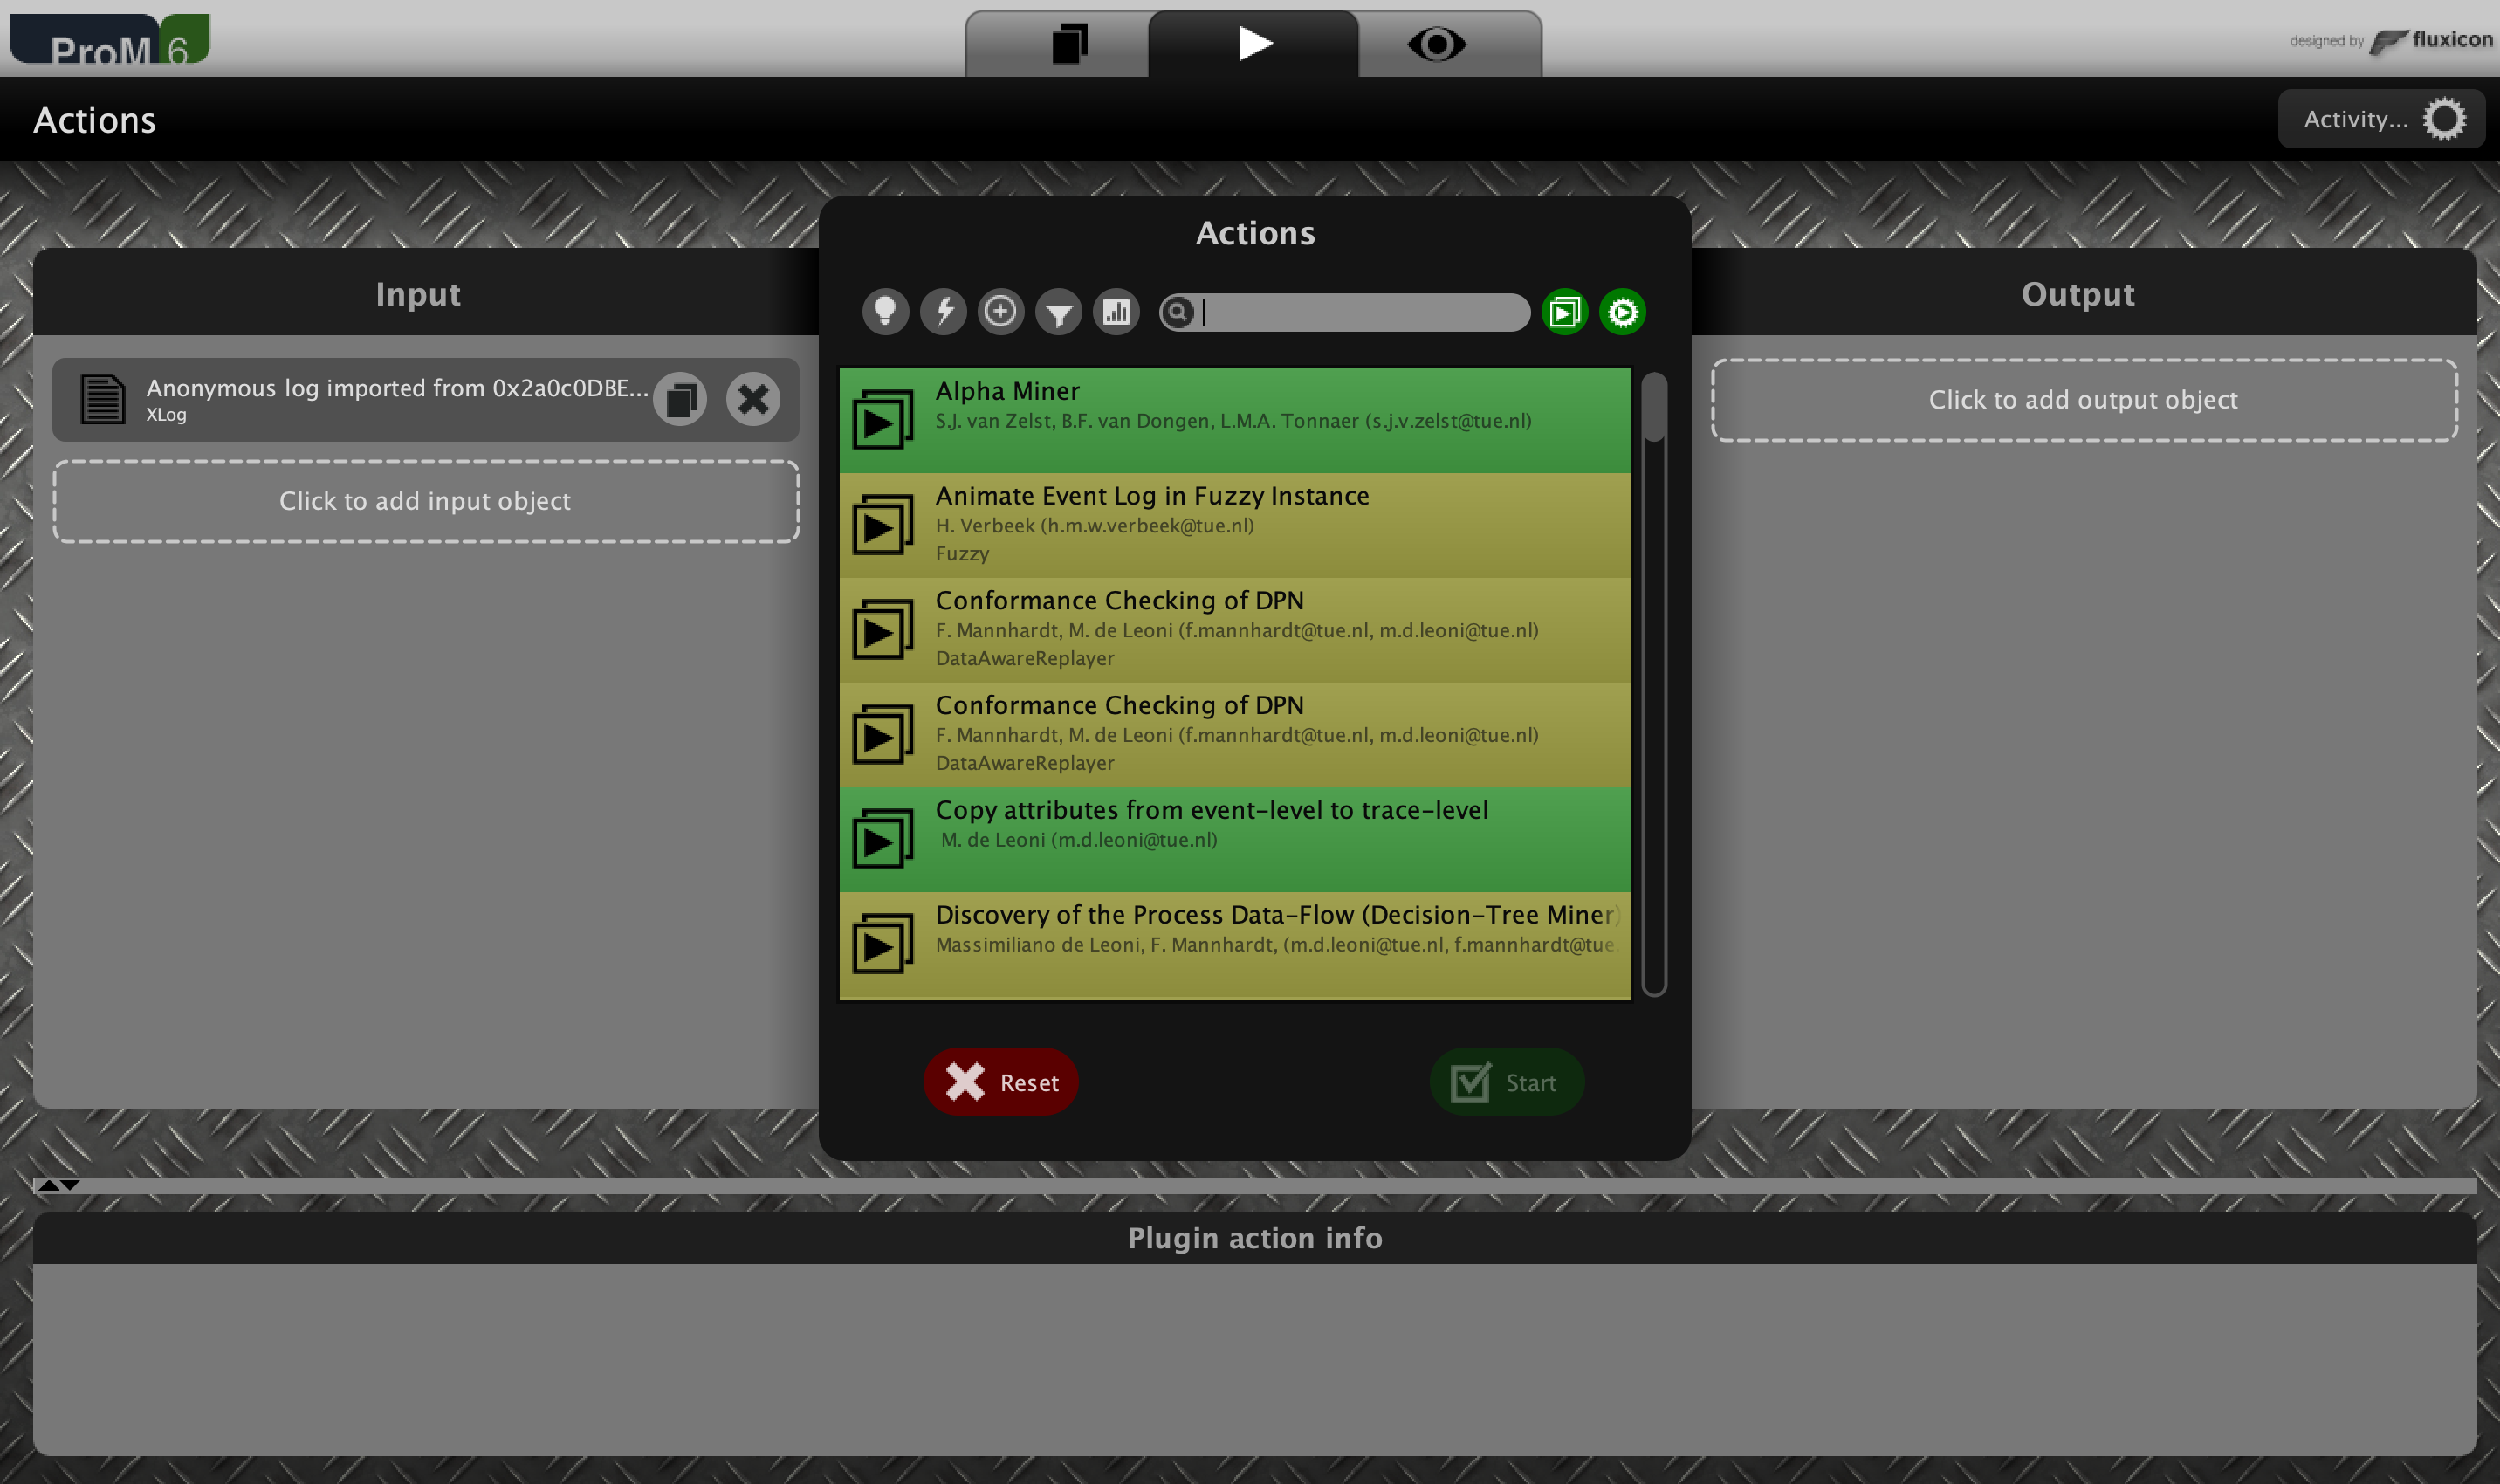
\includegraphics[width=\textwidth]{images/prom_screen_action.png}
    \caption{ProM action view screenshot}
    \label{images:prom_screen_action}
\end{figure}

The action view is the more interesting one: it is its own divided in other three subsections: input objects, feature to apply 
and output objects format/placeholder. In this section is possible to use all ProM techniques (discovery algorithms, 
conformance checking, etc.). The choise of the available actions is filtered based on selected inputs (for example chosen 
a xes file all discovery plugins are available to use but conformance checking cannot be done until the selection of a model to 
compare with log file).

The visualization section change its content based on the currente object selected: it can show a bpmn model, a petri net or 
some parameters measured with some plugin. Here is possible to export current showed data in the desired format.

In general ProM allows to import a lot of type of files (csv, xes, bpmn, etc.) and allow for exports too. It can be also 
used as a conversion tool.

ProM is also open source, this means that every one can write a plugin and make it public for who need it. Over that also its 
java libraries can be used in a custom application making available a powerful framework for developers.

ProM is a great tool, largely used and with a good community; the ui is enough simple to use. Its main disadvantage is its 
granularity: every plugin has a different structure even if their expected behaviour should be the same. In this case the 
great advantage to be an extensible framework became also its main disadvantages creating sometimes inconsistent behaviours 
between plugins.


\subsection{Apromore}
Apromore is an open-source business process analytics platform, supporting the full stack of process mining functionality, 
advanced features for authoring process models and managing process model collections. It is an online tool with different 
node around the world but there is also a desktop version. 

\begin{figure}[!ht]
    \centering
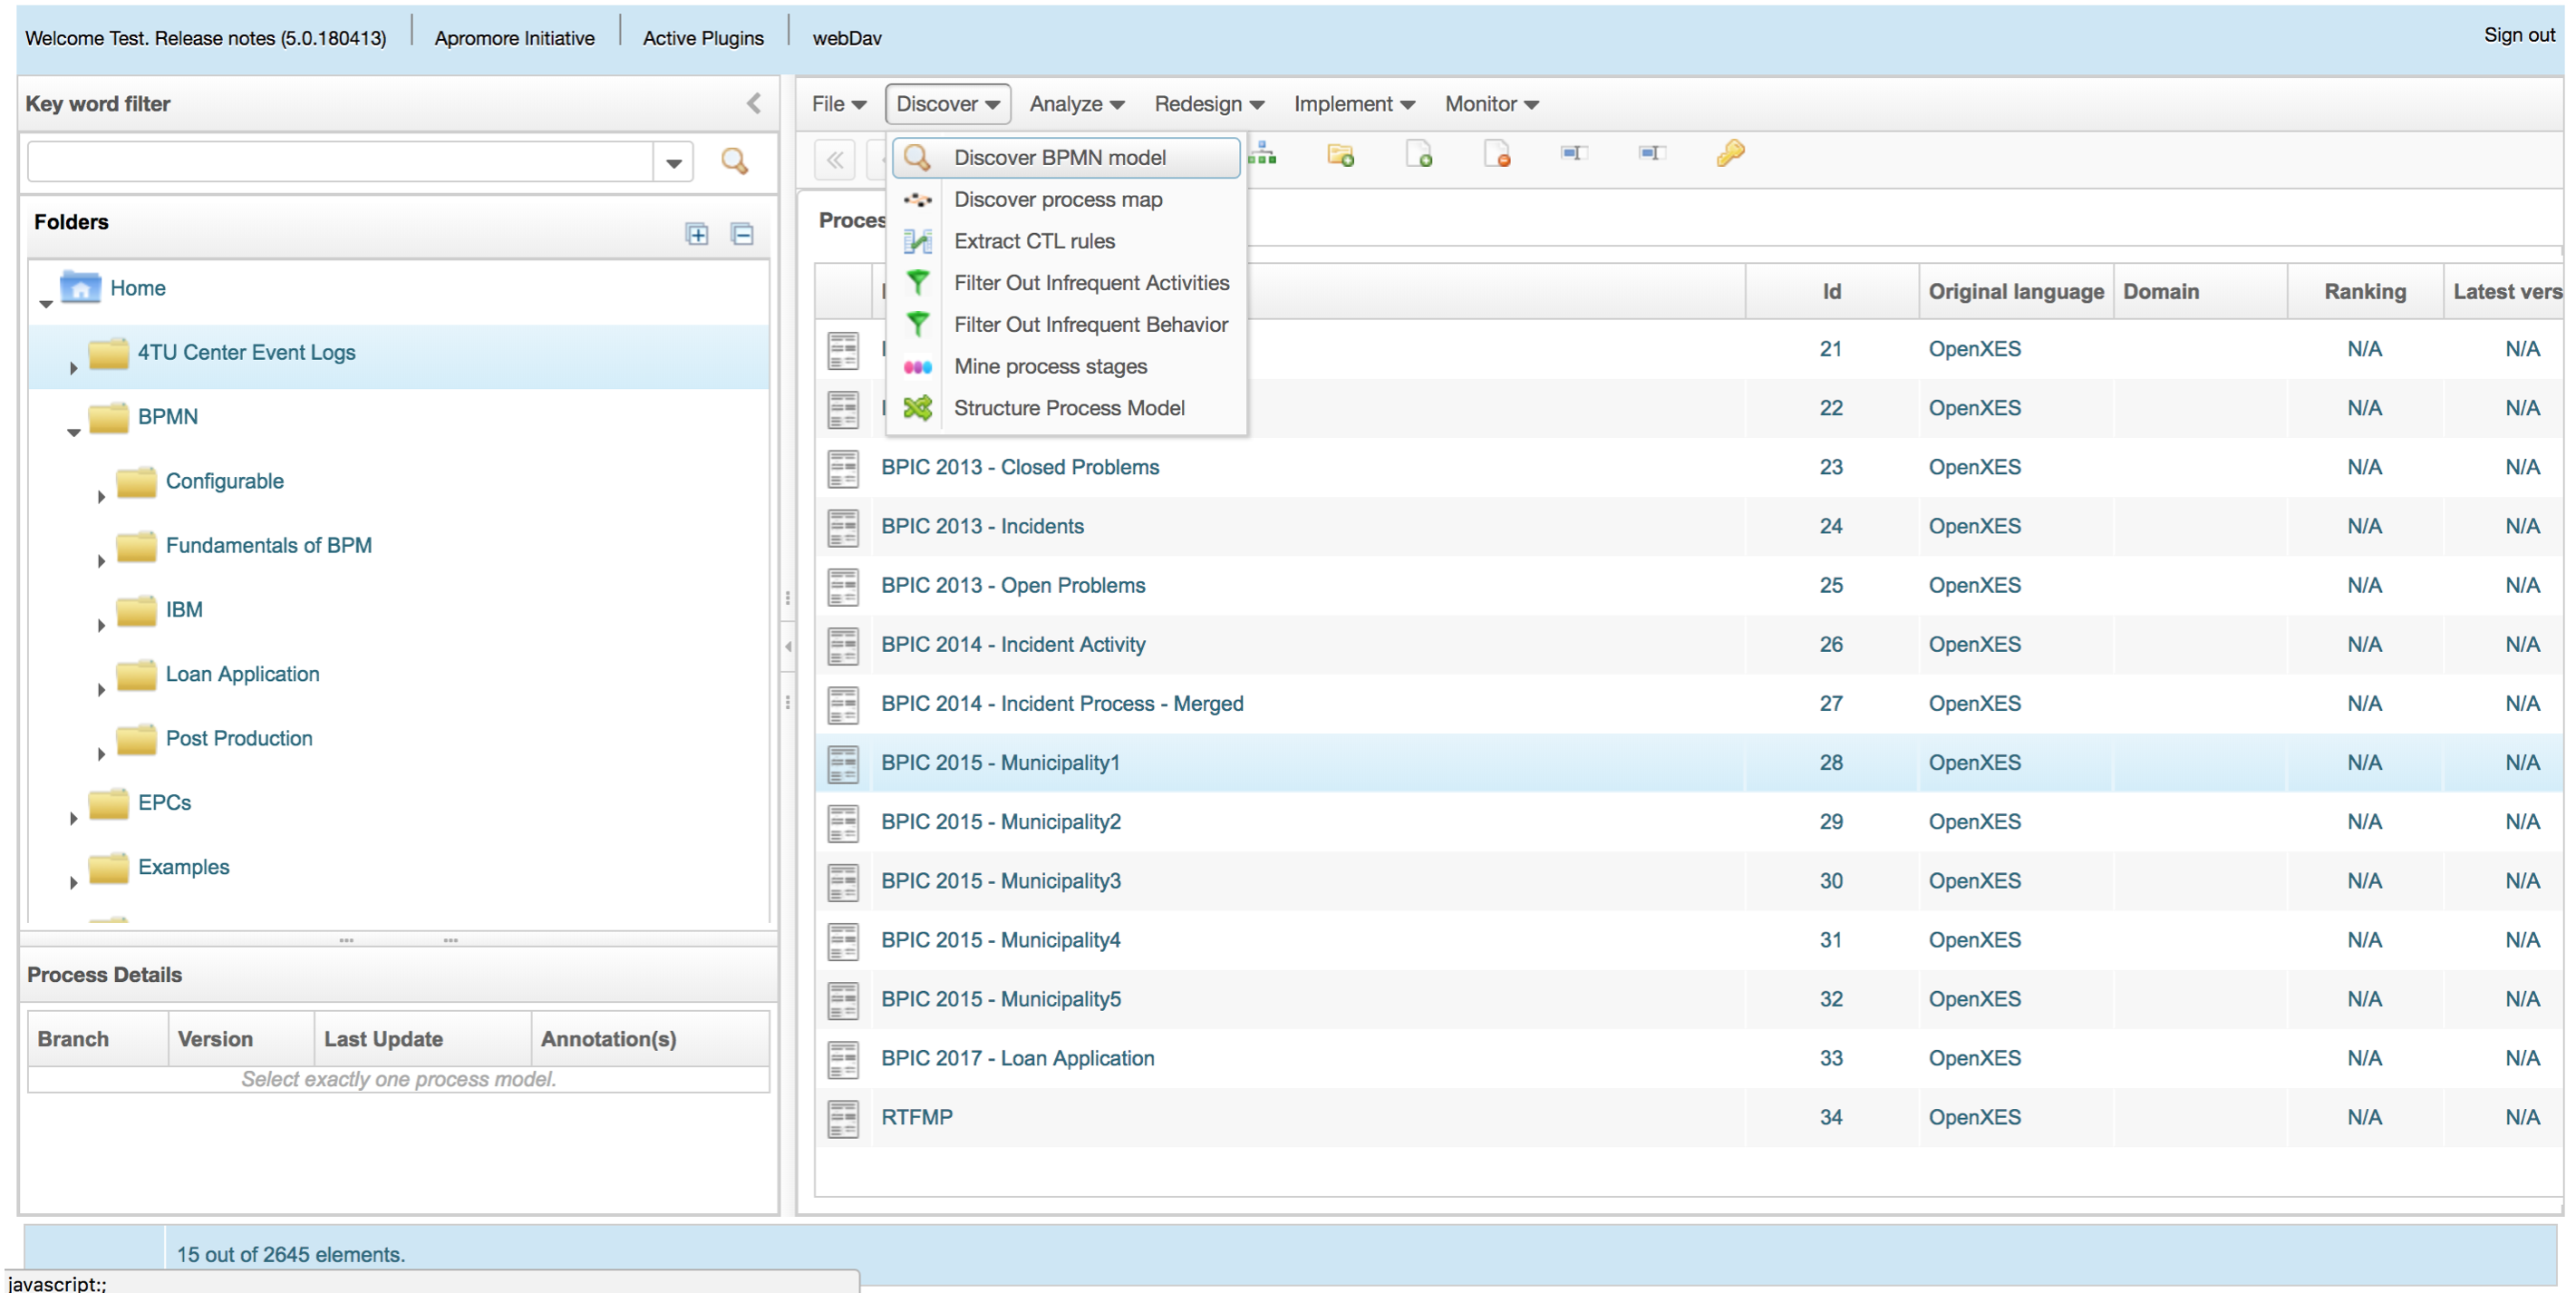
\includegraphics[width=\textwidth]{images/apromore_screen.png}
    \caption{Apromore main window}
    \label{images:apromore_screen}
\end{figure}

In Figure \ref{images:apromore_screen} the main Apromore window is displayed: at a first glance its UI is similar to a file 
server: on the left there is the directories hierarchy, at the center instead there are all files and subdirs of the current 
selected directory. On the top there is a toolbar with all the action that can be executed on the various objects. The 
process model editing commands are in a separate window that is also the visualization part of the tool.

This tool has a rich set of features for the managing of process models: it can be viewed as a process model repository with 
also great capabilities of editing of this models. In this case the set of algorithms supported is a bit different from ProM 
but with some commmon points. There are not a lot of features for quality checking but are supported a rich set of 
interesting capabilities:

\begin{itemize}
    \item animation of event log on top of BPMN models or process map
    \item conformance checking, where model's issues compared to the event log are highlighted
    \item filtering of infrequent activities or behaviors
    \item repair process model to align to event log
    \item train predictive models
\end{itemize}

As ProM even this tool supports all common standards (XES, BPMN, YAWL, etc.) and have a little set of plugins to extend 
the native available features (about 50). Even if this tool is extensible it is a bit less modular compared to ProM. Even in 
this case is possible to use its libraries in a custom project.

In general this is a tool with more features but a bit more complex to use compared to ProM.


\subsection{Disco}
Another tool avaiable in the market is Disco. It was developed by Fluxicon, as ProM, with special attention for user experience 
and speed. There is a basic free version and a complete licensed version. Disco has features for automated process discovery, 
process map animations, detailed statistics, exploration of processes down to single cases or events, filters, import/exports 
in all the main standard formats and in general for project management.

\begin{figure}[!ht]
    \centering
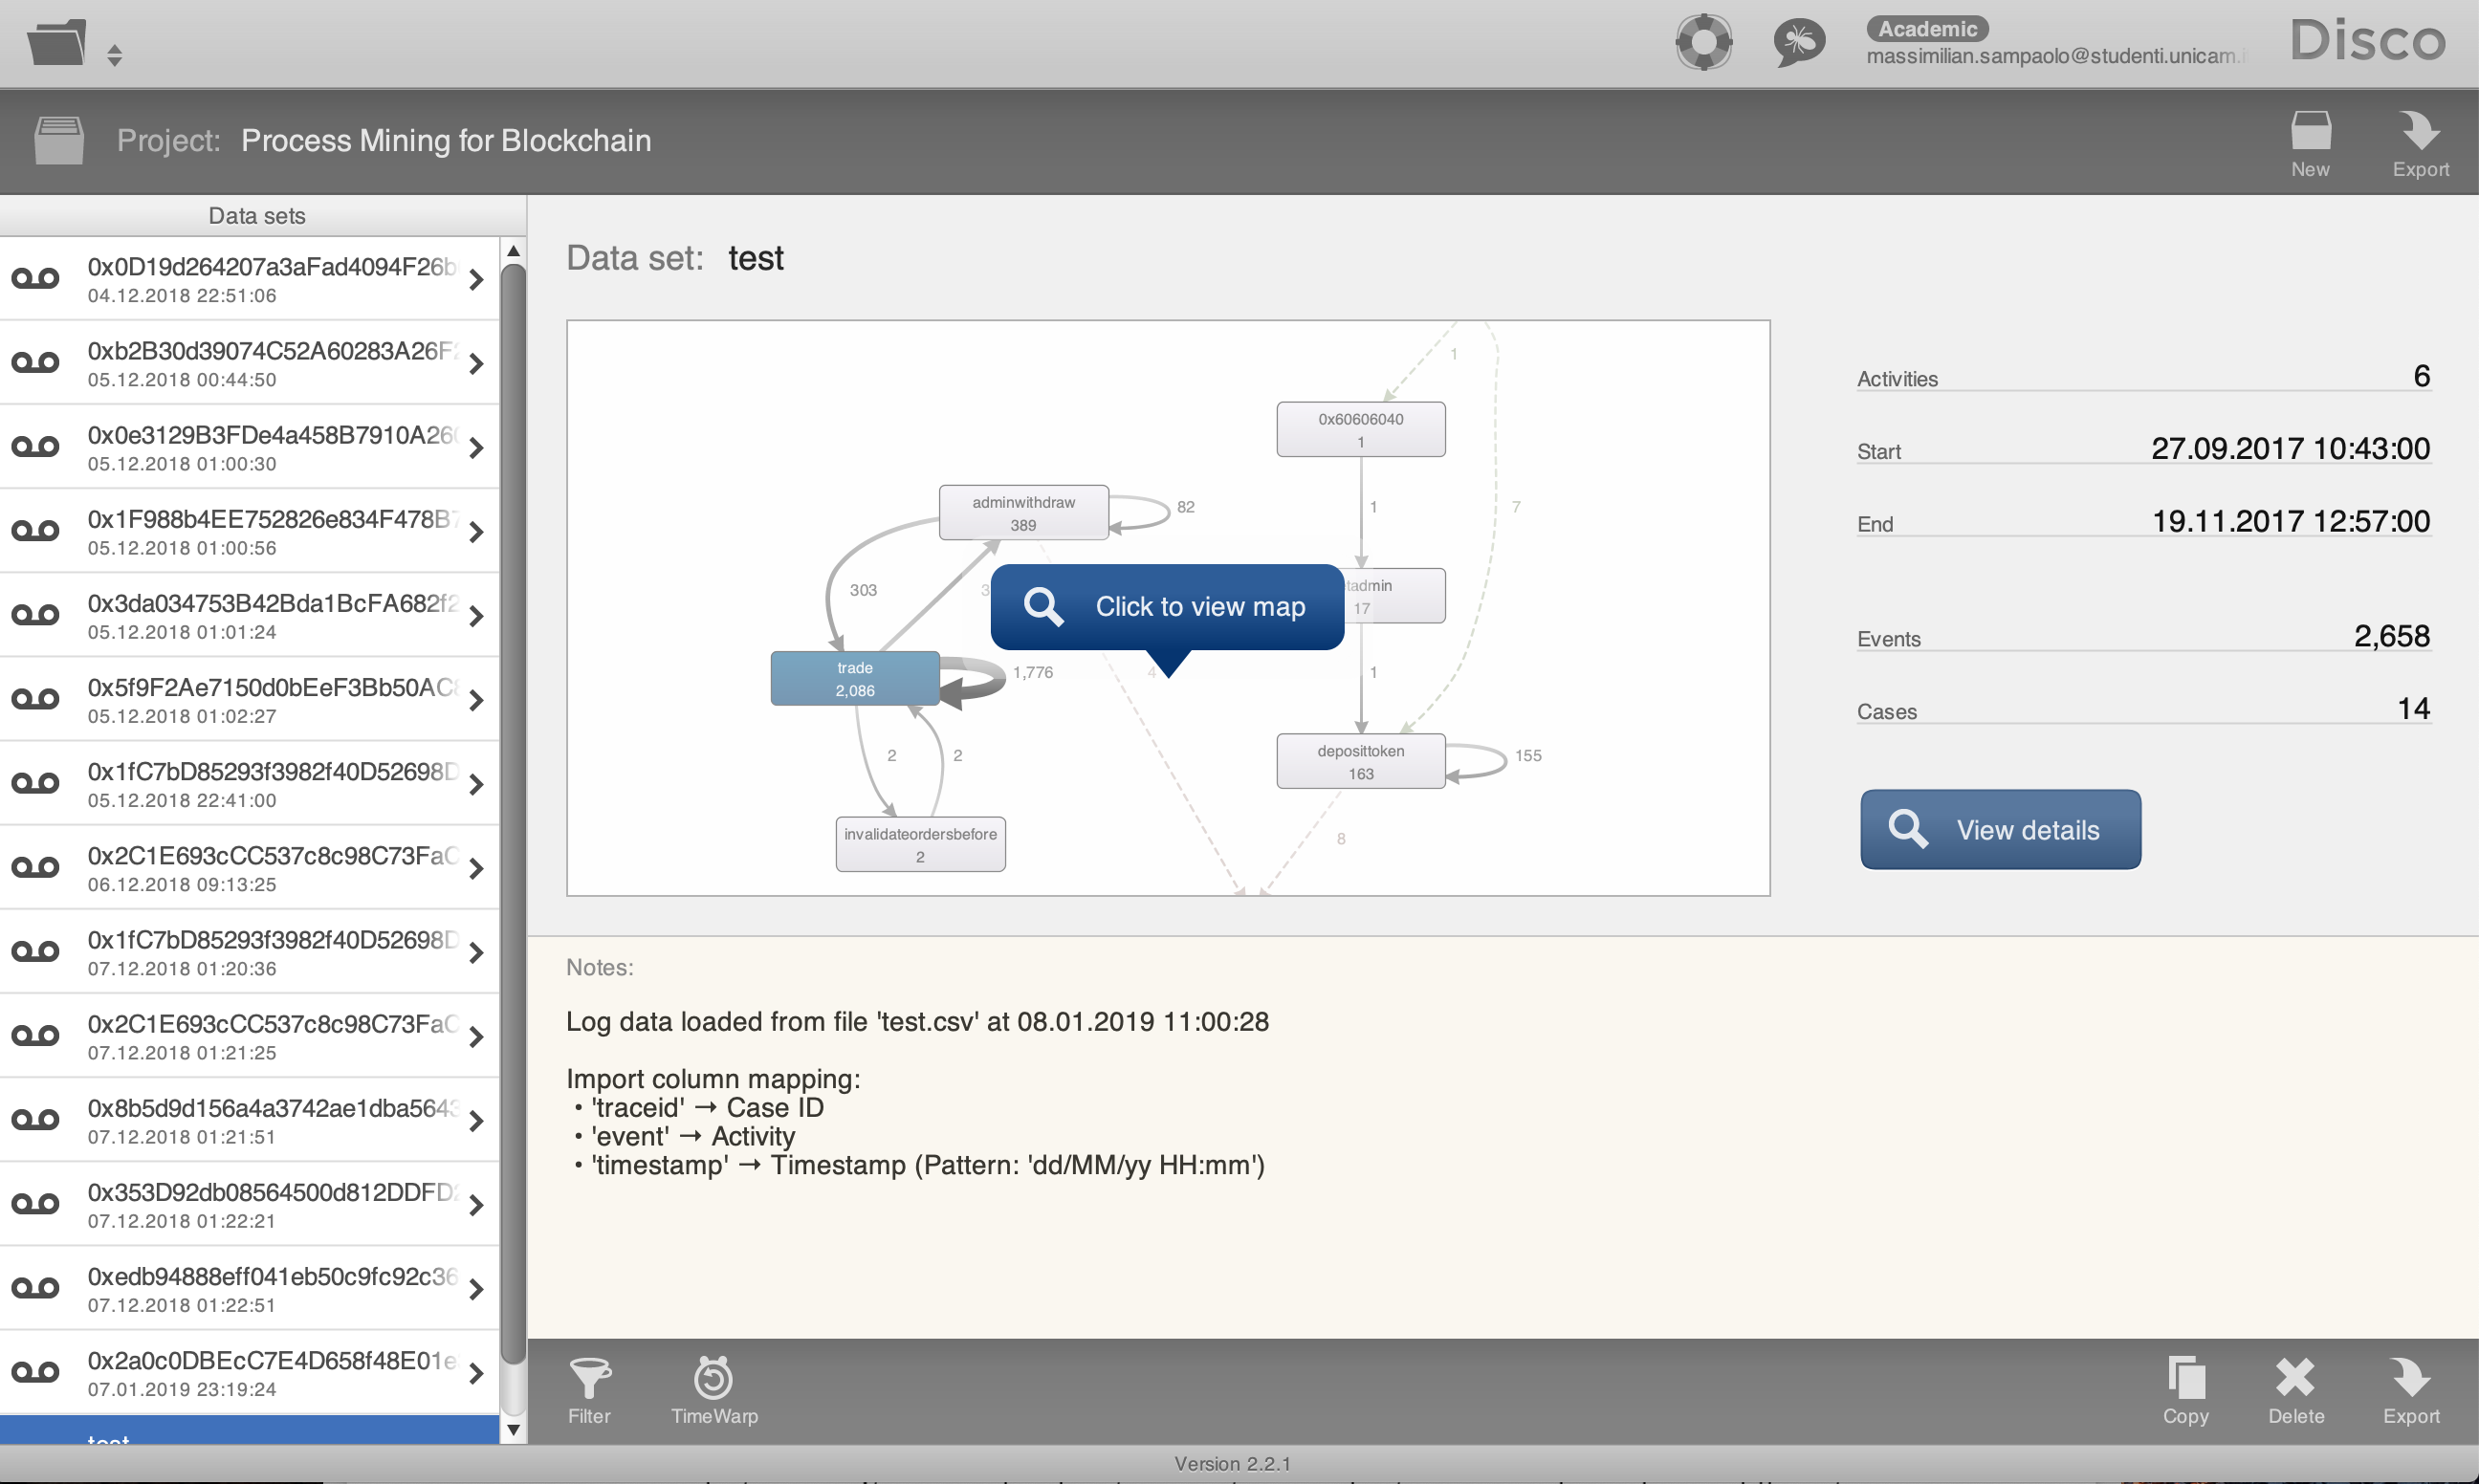
\includegraphics[width=\textwidth]{images/disco_screen.png}
    \caption{Disco main view}
    \label{images:disco_screen}
\end{figure}

In Figure \ref{images:disco_screen} there is a list of imported xes files on the left of the window, a detail of the current 
selection in the center of the window that contains the process map and some basic informations (the number of activities in 
the map, time interval in which the activities are included and the number of traces and events of the event log).

\begin{figure}[!ht]
    \centering
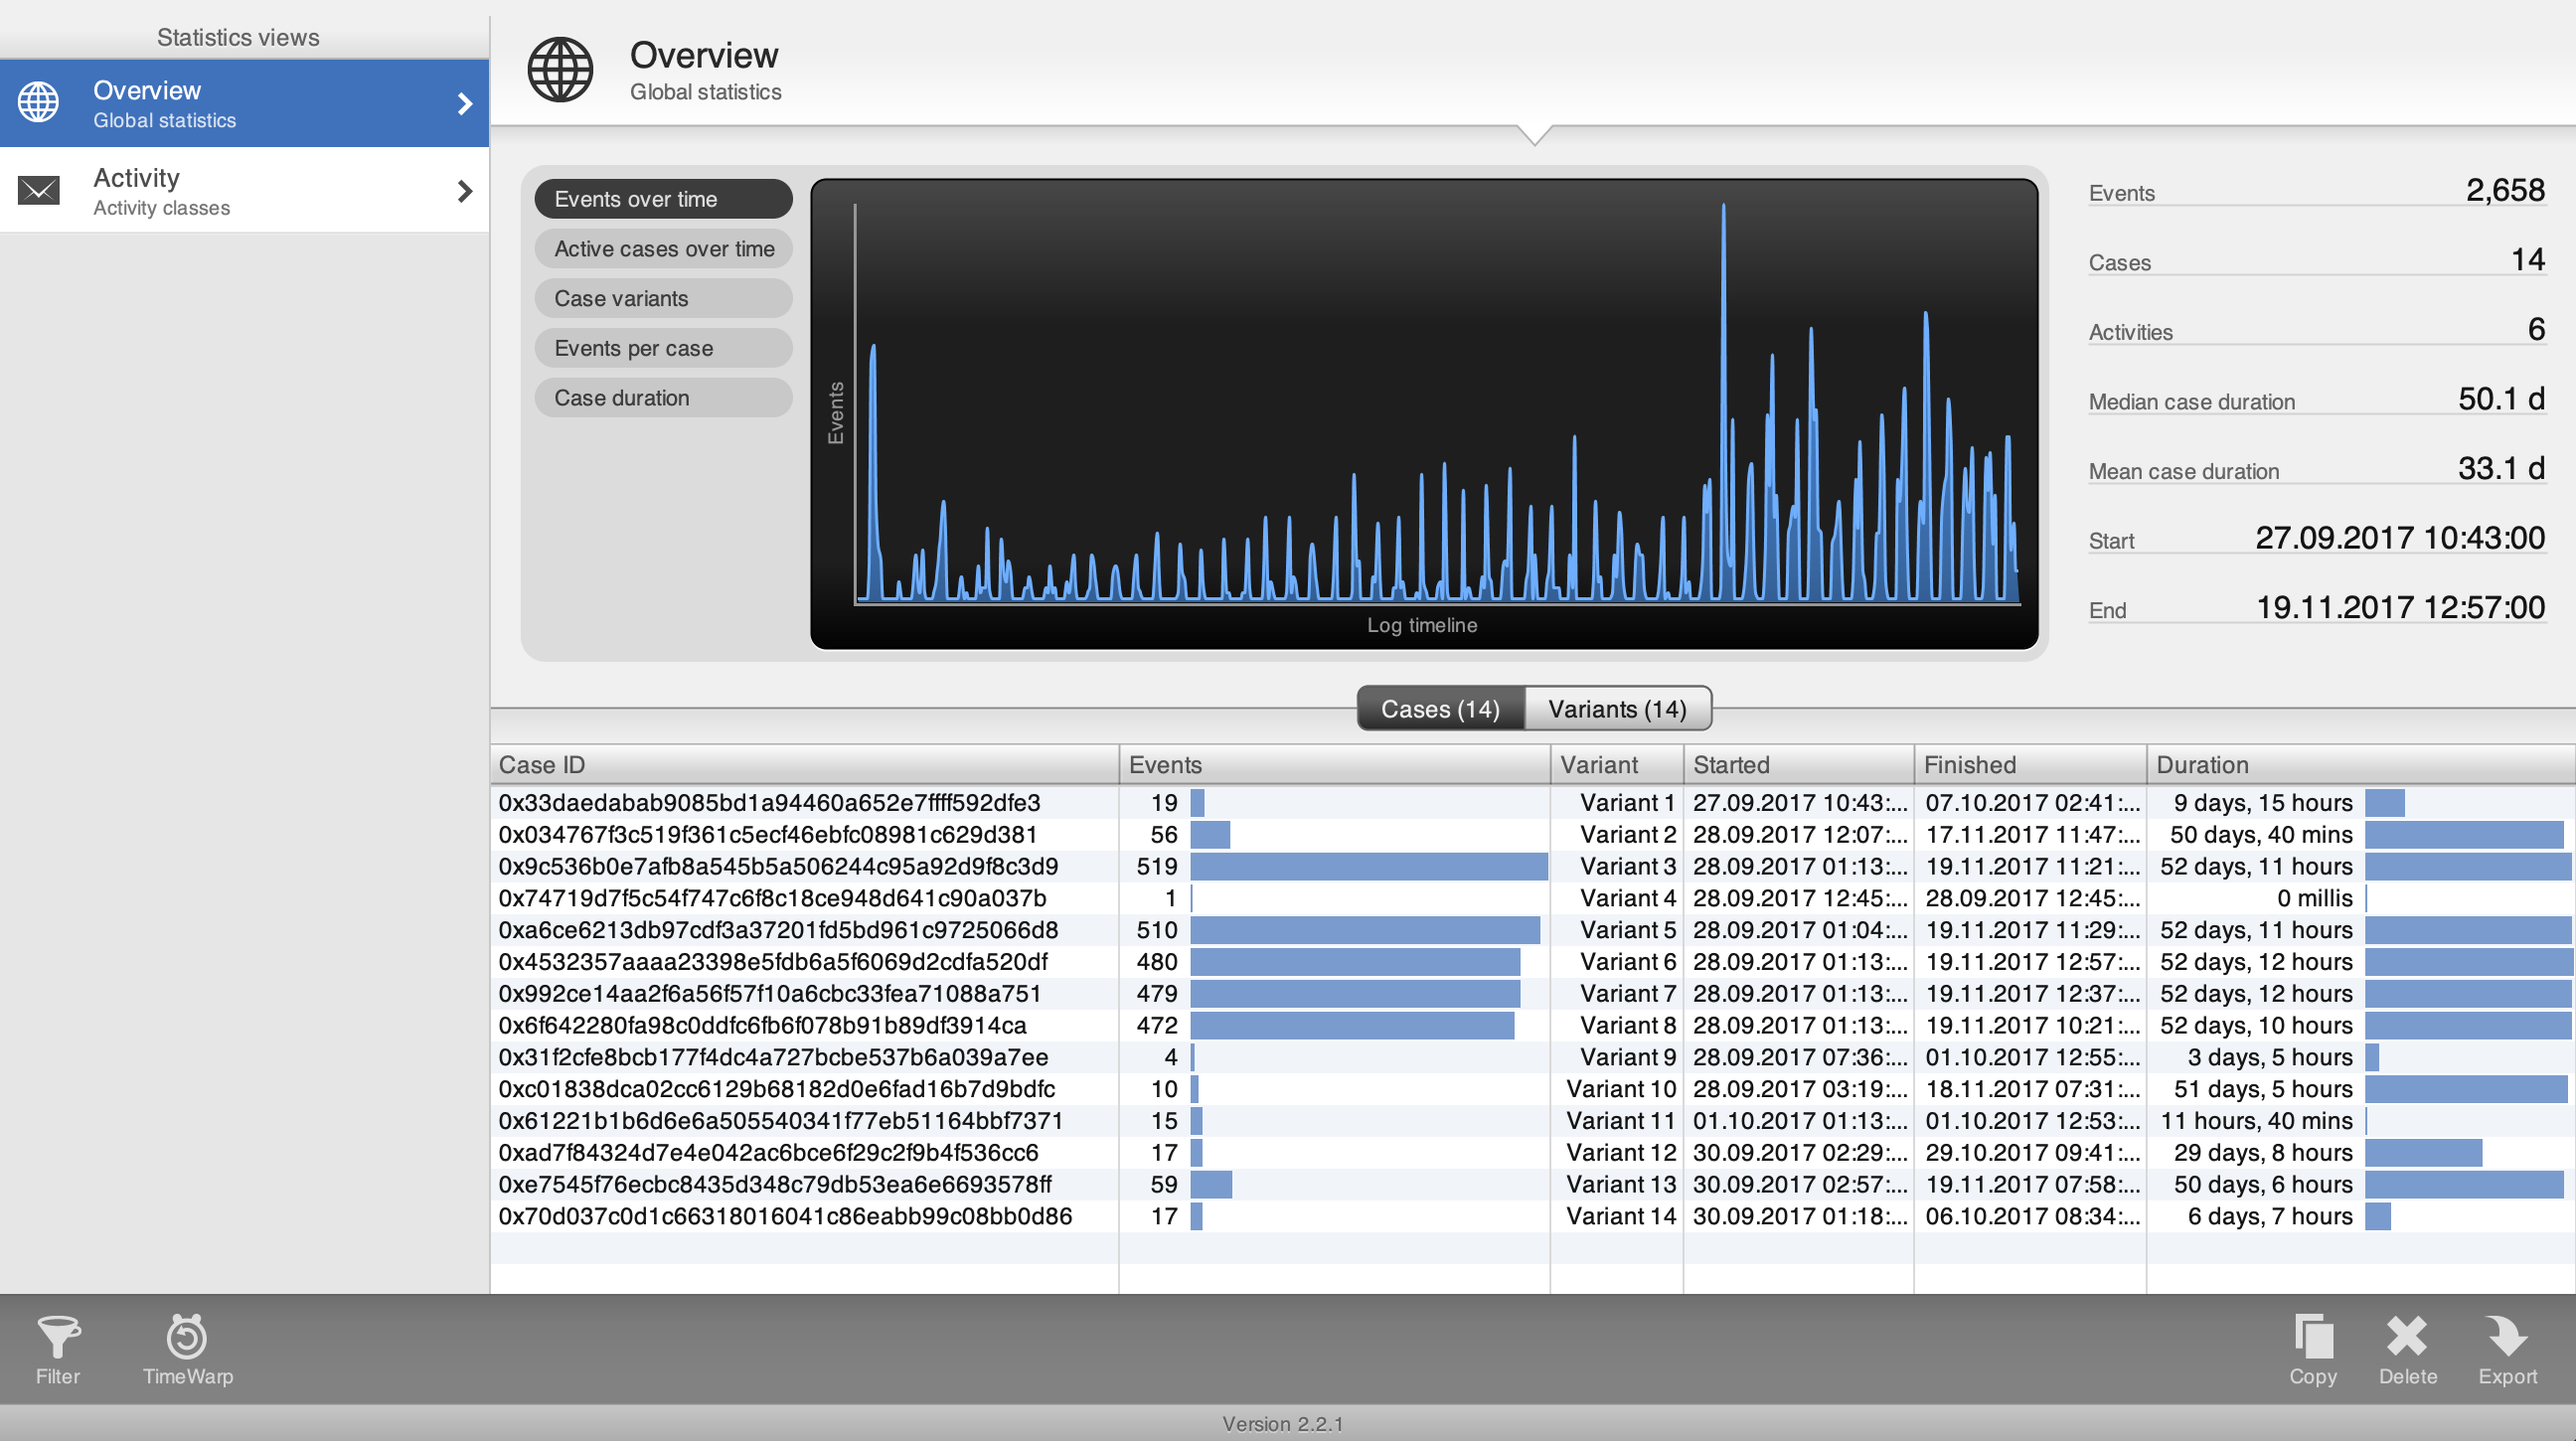
\includegraphics[width=\textwidth]{images/disco_screen_detail.png}
    \caption{Disco detail view}
    \label{images:disco_screen_detail}
\end{figure}

In Figure \ref{images:disco_screen_detail} are shown the details for a specific log/process map in disco: a lot of statistics 
are available with the permission to change the considered time interval. Also a deepening on one of the log event traces can be 
done.
\chapter{Case Studies}
\label{case_studies}

This chapter uses a lot of concepts introduced in the previous ones. Its goal is to extract information from Ethereum combining 
the processing power of process mining and the execution power of the blockchain. The final objective is to find bindings 
between Ethereum transactions and extract the logic that creates them. To do this 3 case studies are presented: the first two 
are games, as usual the game industry is one of the most active in the new technology fields and for this there are a lot of 
games based on Ethereum, making this industry very interesting. Ethereum (and in general the blockchain) can be used in a lot 
of application domains: for this motivation the third case study is not about a game but instead it is about an Exchange.
Moreover this chapter has also a comparison purpose: it compares results obtained in these case studies from three algorithms: 
Split Miner, Heuristic Miner and Inductive Miner.

In Section \ref{case_studies:methodology} is defined the methodology used in the three case studies that are: 
\begin{itemize}
    \item \textbf{RotoHive} described in Section \ref{case_studies:roto};
    \item \textbf{Fomo3D} analyzed in Section \ref{case_studies:fomo};
    \item \textbf{IDEX} deepened in Section \ref{case_studies:idex};
\end{itemize}


\section{Methodology}
\label{case_studies:methodology}

As previously said the final goal of the chapter is to infer the logic which created a set of transactions resident on the 
blockchain. The blockchain technology chosen for this type of analysis is Ethereum because of one of its main components, 
the Smart Contracts. These pieces of software are public and read their code can help to better understand the behaviour of 
a system and bindings between transactions. Over that Ethereum ensures a rich environment, with a good community and many 
tools available.

\begin{figure}[!ht]
    \centering
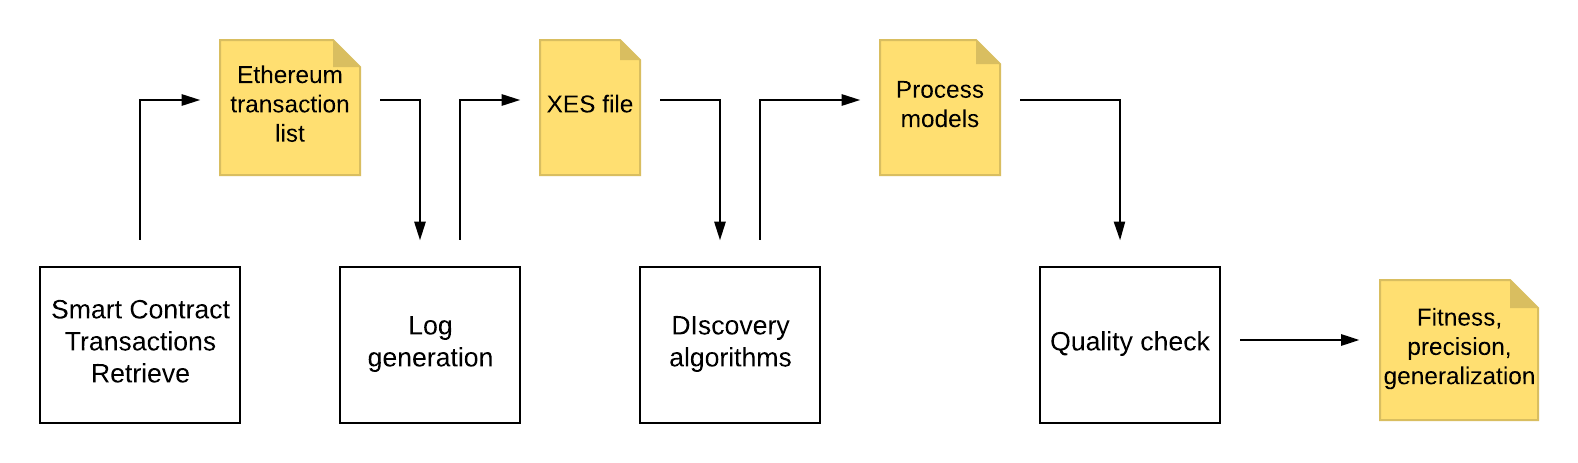
\includegraphics[width=\textwidth]{images/methodology.png}
    \caption{Methodology steps and results}
    \label{images:methodology}
\end{figure}

As shown in Figure \ref{images:methodology} the methodology applied consists of four phases:

\begin{itemize}

    \item \textbf{Smart Contract Transactions Retrieve}. The first phase of the process consists in the retrieve of a list of 
    transactions sended to a Smart Contract. This task is pretty straightforward and its done with a simple console 
    application developed in C\# that exploit an API exposed for free from Etherscan. This API returns a JSON file.

    \item \textbf{Log generation}. The second step of the process is a bit trickier than the previous. Its purpose is to 
    transform the JSON list of transactions in an event log XES file. This activity is done with an intermediate step: in a 
    first place the C\# console application transforms the JSON list in a CSV file and then this CSV is converted in XES using 
    Disco. This intermediate step is needed because there are not any libraries for XES files generation in C\#. The convertion 
    from CSV to XES in Disco is done using the transaction sender as TraceId for the final log and the method of the Smart 
    Contract invoked in that transaction (the field Input Data of the transaction) as Task. This means that in the XES log 
    generated there is one trace for each user that invoked the Smart Contract and inside each trace there is an event/task for 
    each transaction sended from that user.
    The choice of creating traces in the log by grouping transitions by sender ignores the time variable. This can bring to a 
    lost of quality of the resulting log but it is a good compromise between quality and simplicity.

    \item \textbf{Analysis}. The analysis activity start with the selection of the discovery algorithms to use: the chosen set 
    of algorithms is composed from \textbf{Heuristic Miner}, \textbf{Inductive Miner} and \textbf{Split Miner}. This choice is 
    because of the nature of these algorithms: in fact they all use different approach in the discovery process (Directly 
    Follow Graph, divide-et-conquer, Pruning and filtering) so it is a good way to understand which technique fit better in the 
    blockchain environment.
    The choice of the tool is based according to the algorithms used: in fact all these algorithms are available on Apromore and 
    not in other tools (for example ProM does not have an implementation of the Split Miner); moreover Apromore is simple to use, 
    works well and do not need local installation. The analysis activity ends with the application of the choices taken: the XES 
    log is imported in Apromore and then used as input for Split, Inductive and Heuristic Miner algorithms. At the end of this 
    step a collection of BPMN models are available.
    
    \item \textbf{Quality measurement}. The last stage of the process consist in the measure of the goodness of the results 
    obtained: as explained in chapter \ref{process_mining} the quality of a discovered model in reference to the log from which 
    it was generated can be measured using Fitness, Precision and Generalization.
    Generally these values are calculated starting from a model expressed as Petri Net. This means that a tool that converts 
    BPMN to Petri Net is needed. ProM offer a plugin called ``Convert BPMN diagram to Petri net (control-flow)" that allow for 
    this convertion. Since this is a crucial step this convertion must be verified and this can be done using rules defined in 
    \cite{DBLP:journals/BPMNtoPN} and showed in Figure \ref{images:BPMNtoPN_rules}.
    Over that ProM also has a plugin for the replay of a log on a petri net (``Reply a Log on a Petri Net for Conformance 
    Analysis"): this plugin generates a set of metrics and among them there is also the ``trace fitness" that is the fitness 
    measure. The evaluation of precision and generalization is done with a third plugin (``Measure Fitness/Generalization") that 
    starts from the result of the previous one.
    
\end{itemize}

\begin{figure}[!ht]
    \centering
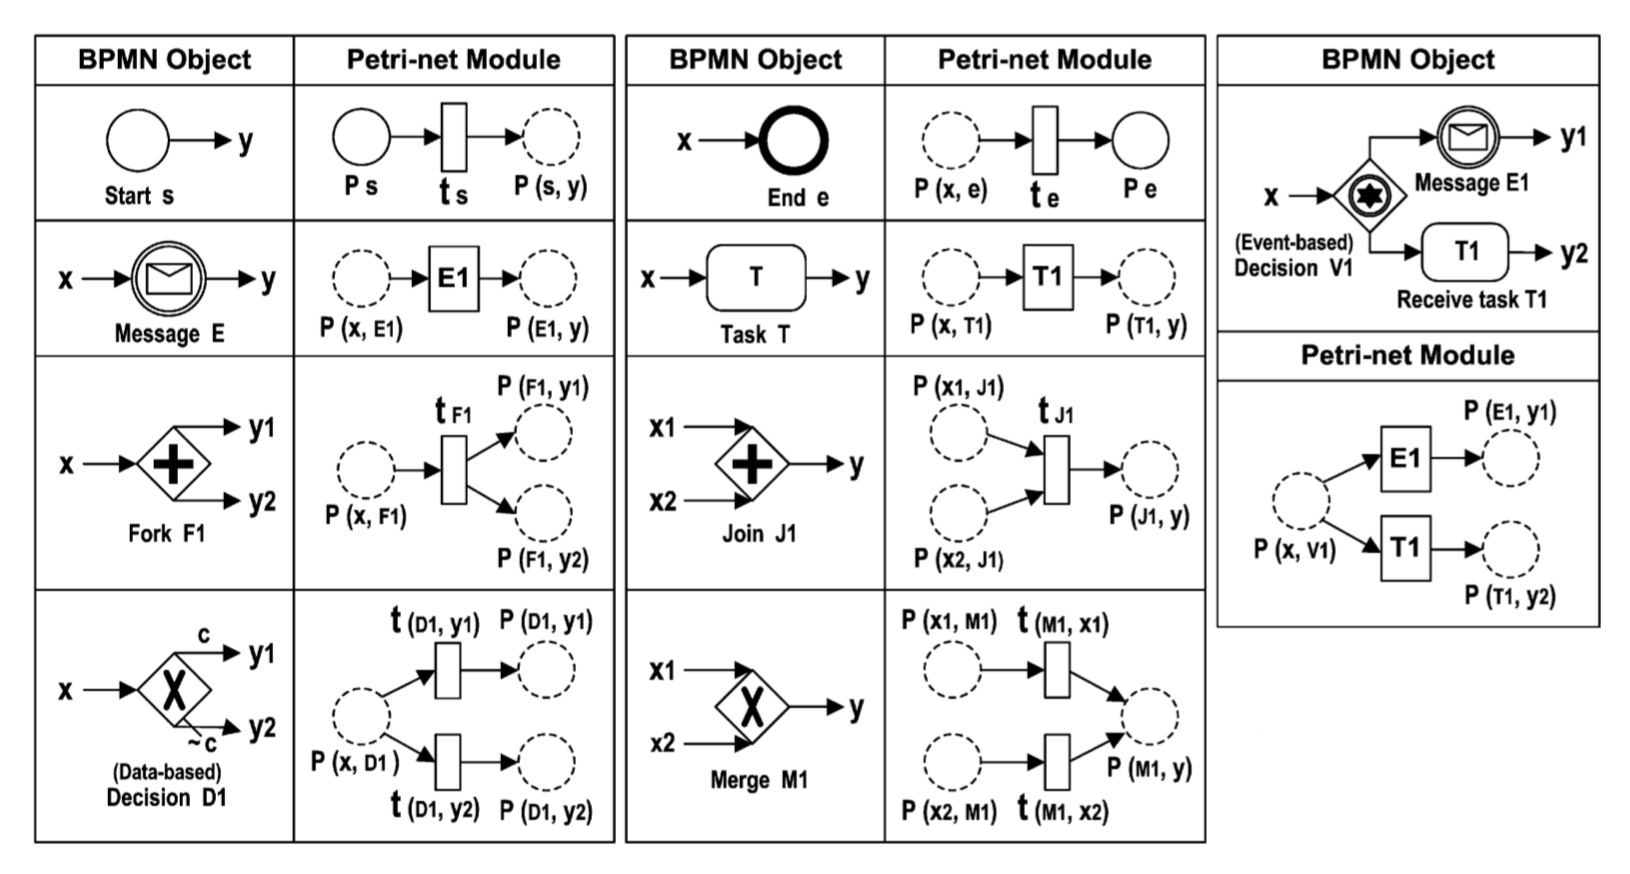
\includegraphics[width=\textwidth]{images/BPMNtoPN_rules.png}
    \caption{BPMN to Petri net conversion rules \cite{DBLP:journals/BPMNtoPN}}
    \label{images:BPMNtoPN_rules}
\end{figure}

At this point the complete process is ready to be applied to some case studies: first of all the download of the Smart Contract 
transactions, after that the building of a log starting from these transactions, then the analysis of these logs using 
different algorithms in Apromore and finally, the evaluation of the results with ProM.
In next sections these case studies are presented: the first two are games (RotoHive and Fomo3D) and the last one is an 
Exchange (IDEX).


\section{RotoHive}
\label{case_studies:roto}
RotoHive (https://www.rotohive.com) is a new type of fantasy sports site that runs weekly tournaments. It is similiar to the ``Fantacalcio", every 
Tuesday a new tournament starts and users are asked to rank NFL players by position (Quarterbacks, Running Backs, 
Wide Receivers, Tight Ends and Team Defenses) based on projected performance for the week. RotoHive user submissions are 
then rated against live player performances on Sunday and Monday night. At the end of Monday Night Football, top performing 
RotoHive users are paid for their accurate player rankings. This process then repeats on Tuesday morning when the next 
weekly tournament begins. Roto can then be staked to user submissions to win a portion of a separate weekly Ethereum prize 
pool.

The log built for RotoHive has more than 3000 events grouped in 13 different traces (this means 13 different users that played the game).
This means that even if this log considers few users the behaviour of each user with the game is quite complex with a lot of 
interactions with Ethereum (a lot of events in the log).

Figures \ref{images:roto_split}, \ref{images:roto_inductive} and \ref{images:roto_heuristic} show the resulting process models 
obtained applying, respectively, Split Miner, Inductive Miner and Heuristic Miner.

\begin{figure}[!ht]
    \centering
    \makebox[\textwidth] { 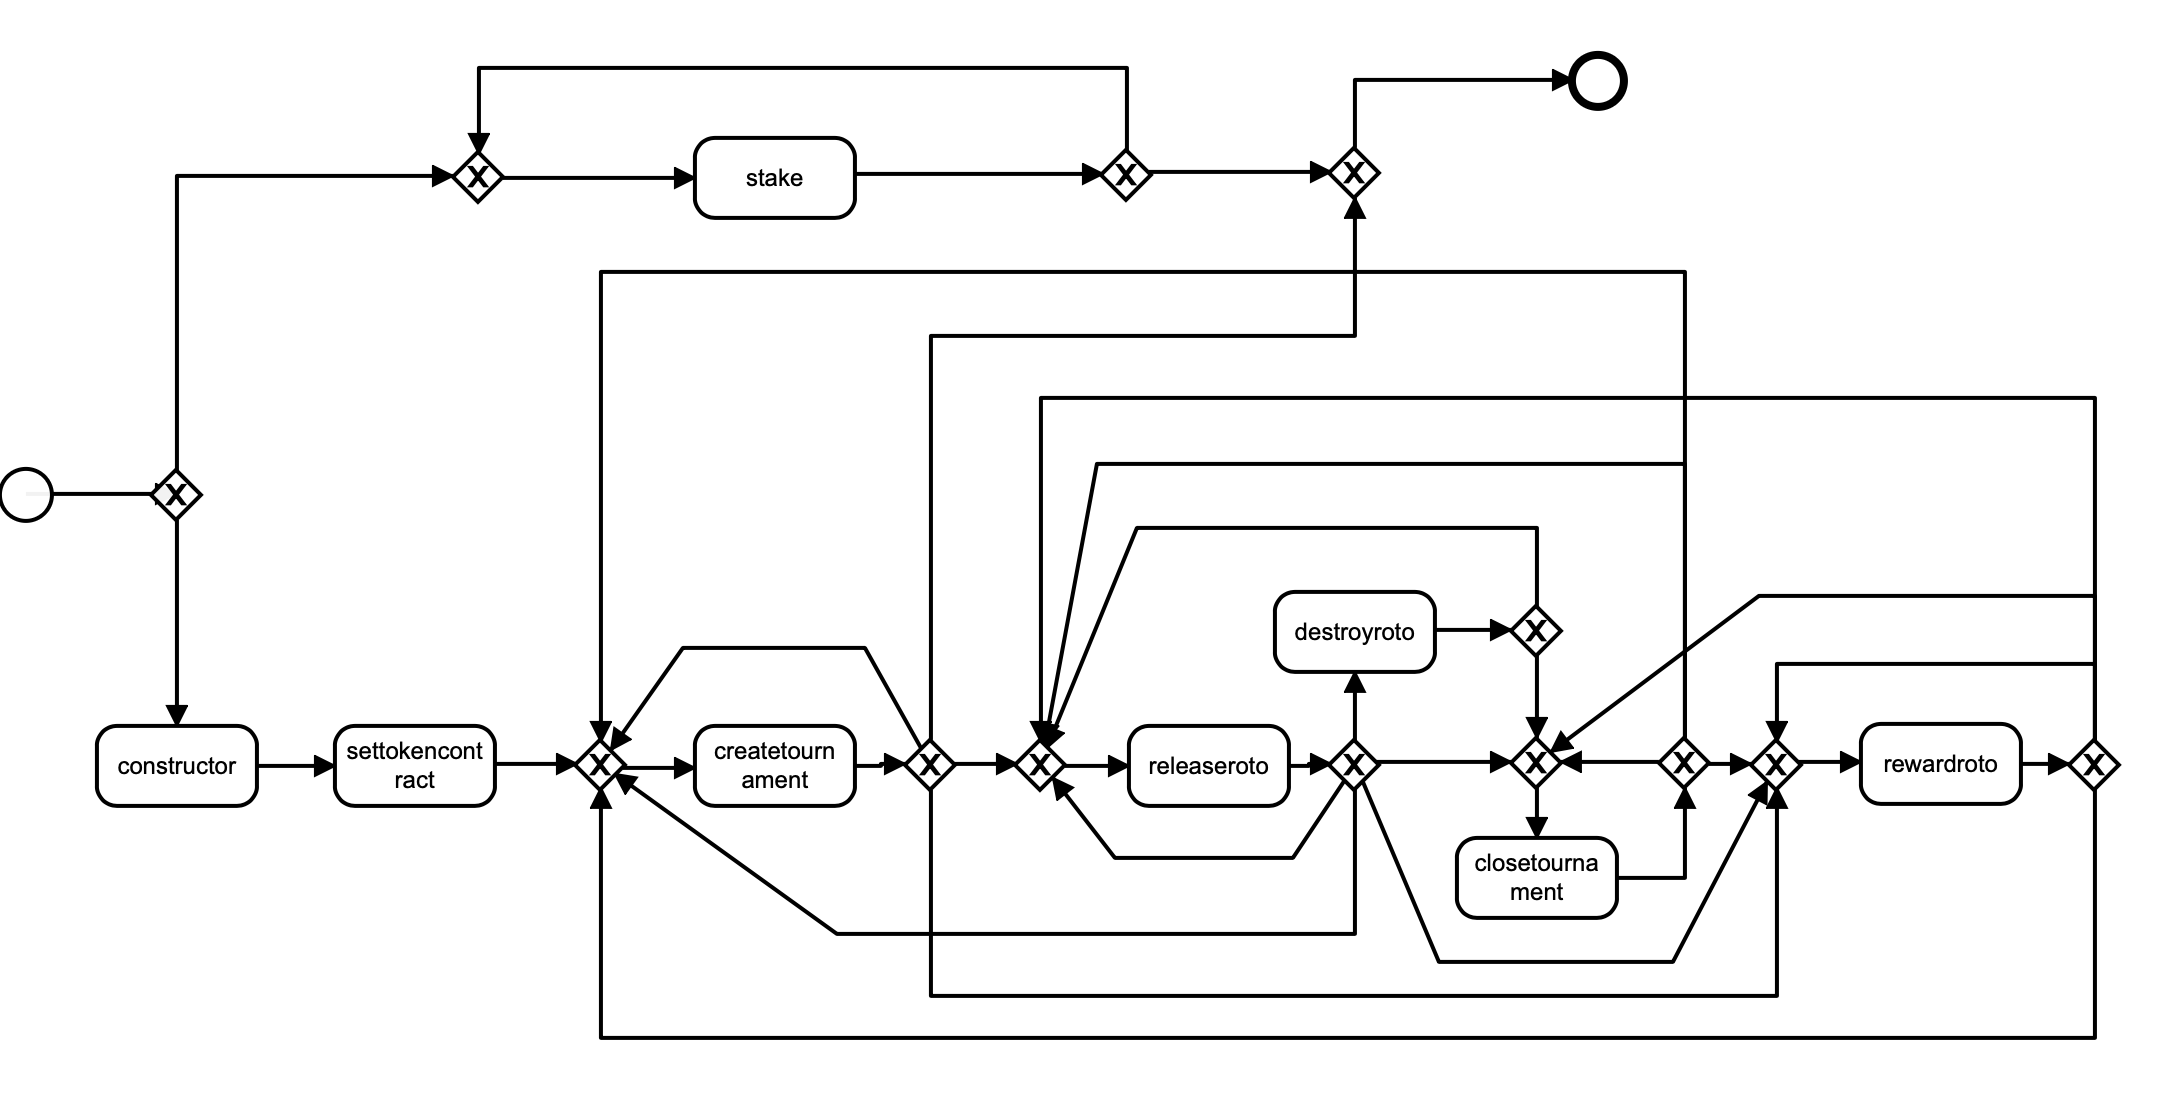
\includegraphics[width=1.2\textwidth]{images/roto_split.png} }
    \caption{RotoHive split miner}
    \label{images:roto_split}
\end{figure}

\begin{figure}[!ht]
    \centering
    \makebox[\textwidth] { 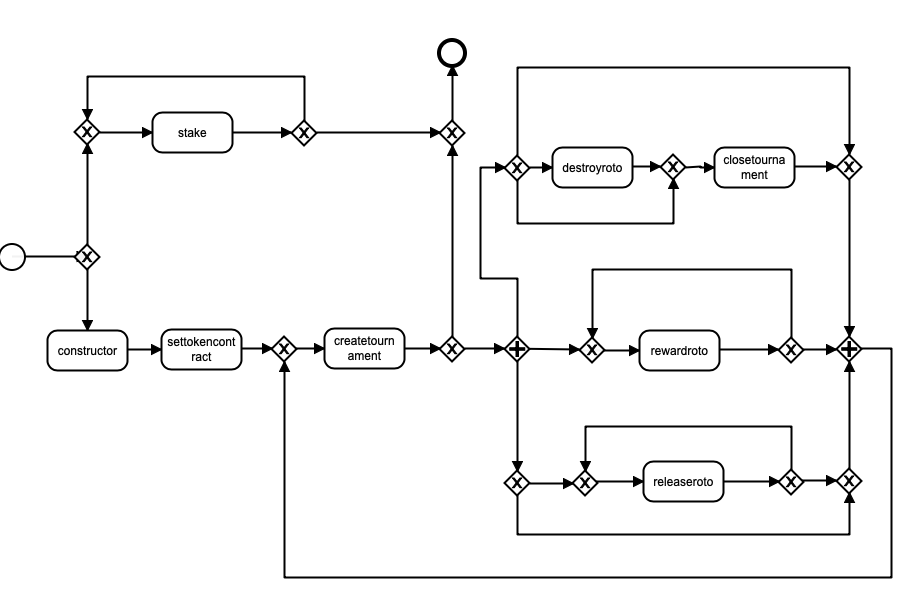
\includegraphics[width=1.2\textwidth]{images/roto_inductive.png} }
    \caption{RotoHive inductive miner}
    \label{images:roto_inductive}
\end{figure}

\begin{figure}[!ht]
    \centering
    \makebox[\textwidth] { 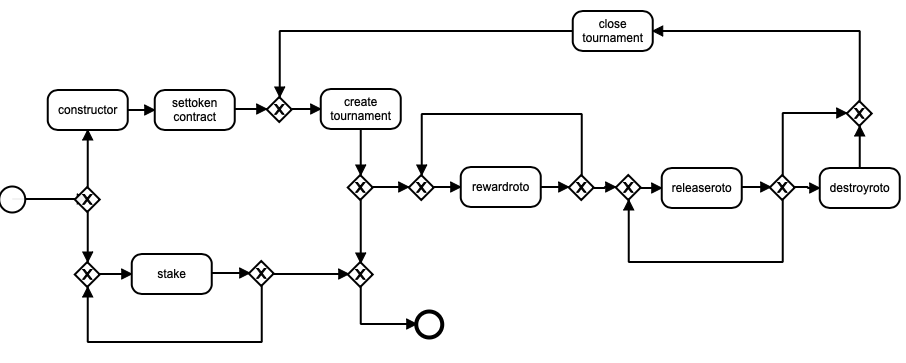
\includegraphics[width=1.2\textwidth]{images/roto_heuristic.png} }
    \caption{RotoHive heuristic miner}
    \label{images:roto_heuristic}
\end{figure}


In general in the model there is a main fork that split the process for user: a first part is for common users that can only 
stake their Roto in order to win Ether and a second part that is for the admin of the system who can create a tournament, 
distribute Roto to winners or destroy Roto for bad performances and than close the tournament in a weekly cycle.

Table \ref{tables:roto} shows the results of the qualitative measures on the models:

\begin{center}
    \label{tables:roto}
    \begin{tabular}{ | l | c | c | c | c |}
        \hline
        \textbf{Algorithm} & \textbf{BPMN to PN} & \textbf{Fitness} & \textbf{Precision} & \textbf{Generalization} \\ 
        \hline
        Split Miner & Ok & 1 & 0.20453 & 0.99892 \\ 
        \hline
        Inductive Miner & Ok & 0.99995 & 0.60294 & 0.99496 \\
        \hline
        Heuristic Miner & Ok & 0.99940 & 0.49889 & 0.99889 \\
        \hline
    \end{tabular}
\end{center}

We can see that Fitness and Generalization values a pretty high in each algorithm while Precision is more variable and in 
general values are smaller. The evaluation of the conversion between BPMN and Petri Net is done using rules described 
previously. In general all the three models represents quite well the application domain but those discovered with Split Miner 
and Inductive Miner are too confusing. Simplicity is an important aspect and for this motivation the Heuristic Miner is the 
algorithm that performed better in this case study.


\section{Fomo3D}
\label{case_studies:fomo}

Here's Fomo3D (https://exitscam.me/play) in a nutshell:

\begin{itemize}
    \item This is a lottery game in which the last person to buy a key at the end of a round wins the jackpot!
    \item During a round, people can purchase 1 or more keys which resets the timer marking them as the current leader. With each key purchase during the round, the key price increases slightly.
    \item Players receive a stream of passive income from the game as keys are bought during the round.
    \item When the timer reaches zero, last person to buy a key wins! (F3D players/P3D holders get a piece too!)    
\end{itemize}

With a few cool game mechanics:

\begin{itemize}
    \item There are two different game modes with distinct rules and round durations: Long and Soon.
    \item Players can select from one of four teams which determine certain rules in the round.
    \item P3D holders receive dividends on each key purchase and at the end of the round.
    \item Players can buy a vanity URL and/or refer your friends to the game for extra rewards.
    \item Buying keys offers you a \% chance to receive an ``airdrop" winning ETH from a growing side-jackpot!
\end{itemize}

At the end of the round, the ETH in the jackpot is divvied up: the winner receives half of the jackpot, with the rest split 
between all F3D players as well as to P3D holders. The specific way the ETH is divided between the F3D participants 
and the P3D holders depends on which team the winner was representing. 

The resulting log in this case contains more traces than RotoHive (so more users for the game), about 40, but with less 
interactions with the smart contract in fact on average there are only three events per each trace.

In Figures \ref{images:fomo_split}, \ref{images:fomo_inductive} and \ref{images:fomo_heuristic} the resulting models 
obtained after the analysis based on, respectively, Split Miner, Inductive Miner and Heuristic Miner.

\begin{figure}[!ht]
    \centering
    \makebox[\textwidth] { 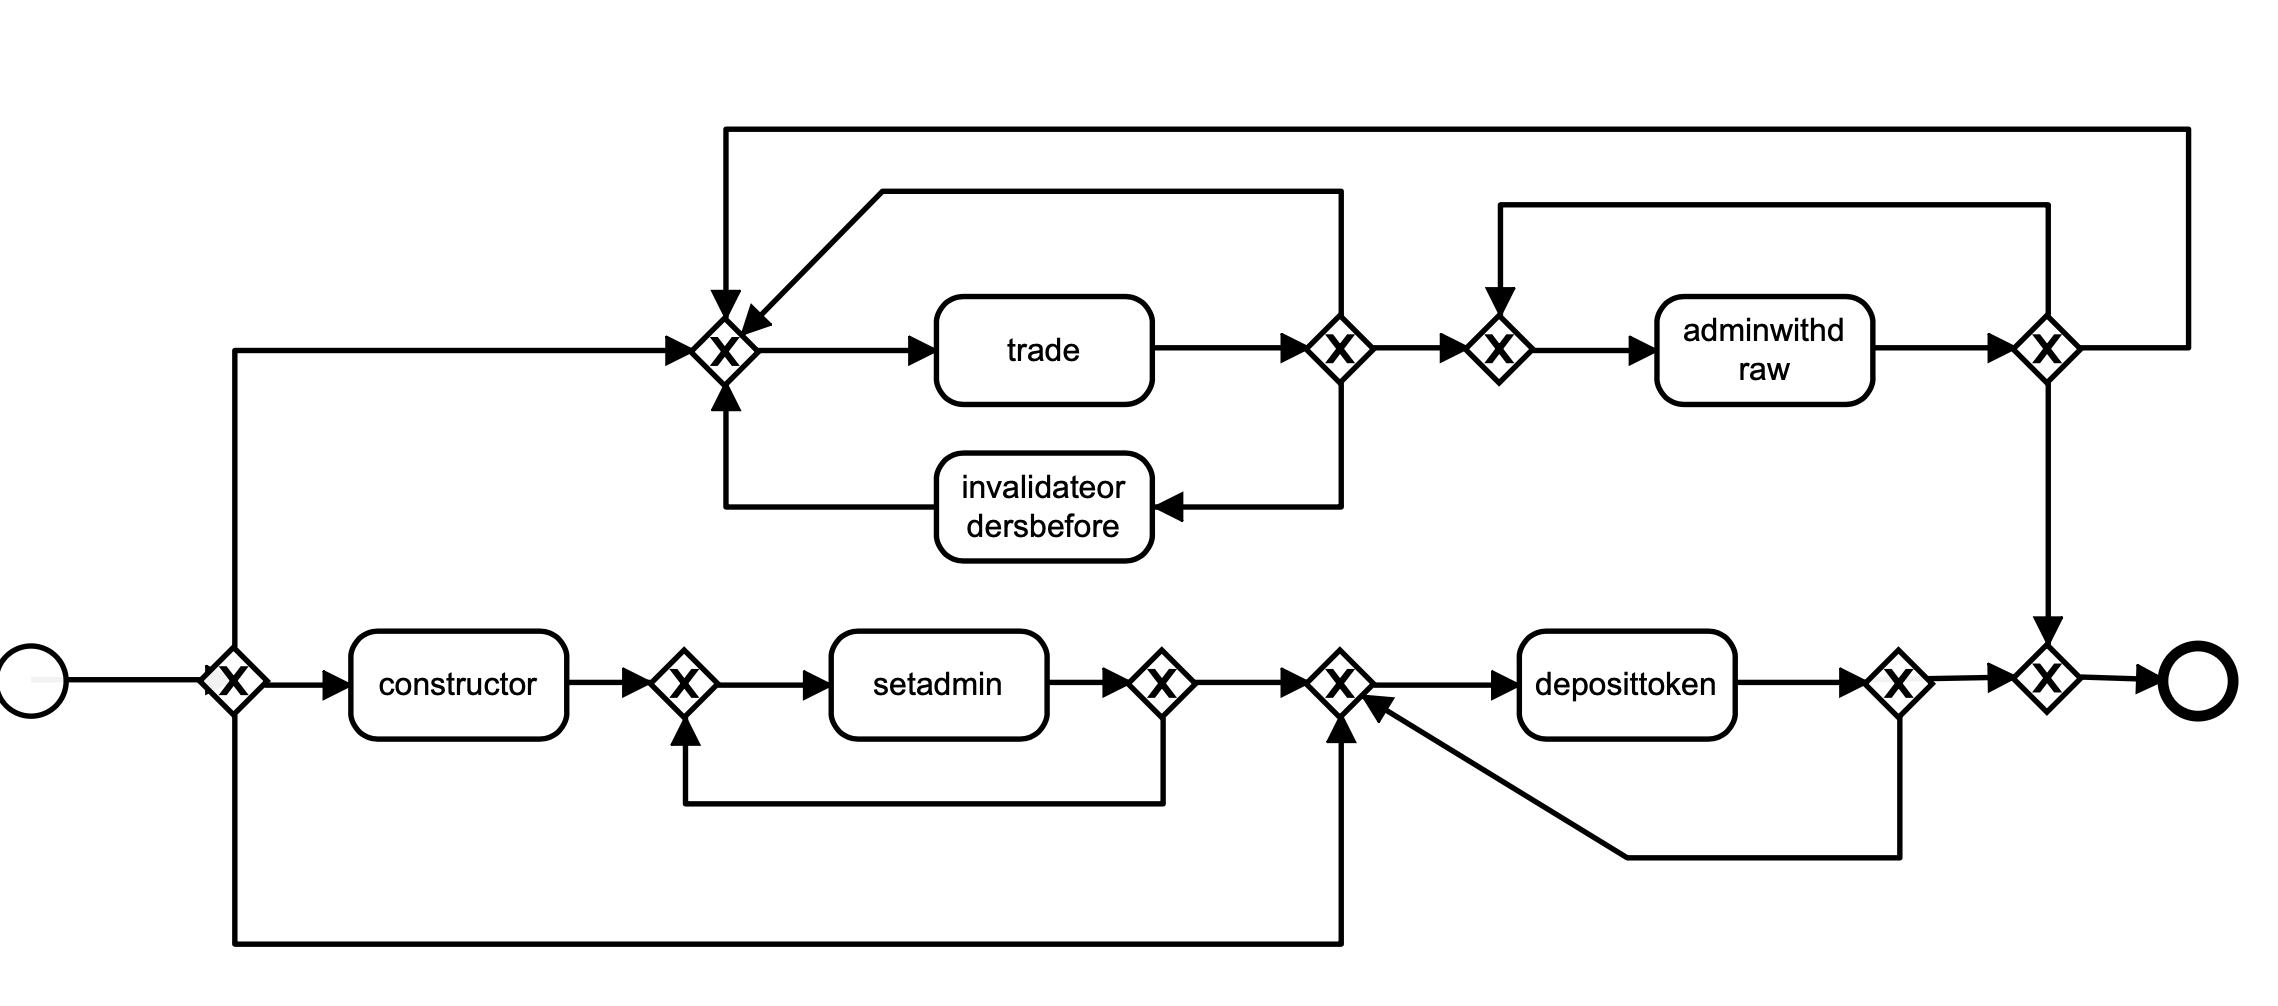
\includegraphics[width=1.2\textwidth]{images/fomo_split.png} }
    \caption{Fomo3D split miner}
    \label{images:fomo_split}
\end{figure}

\begin{figure}[!ht]
    \centering
    \makebox[\textwidth] { 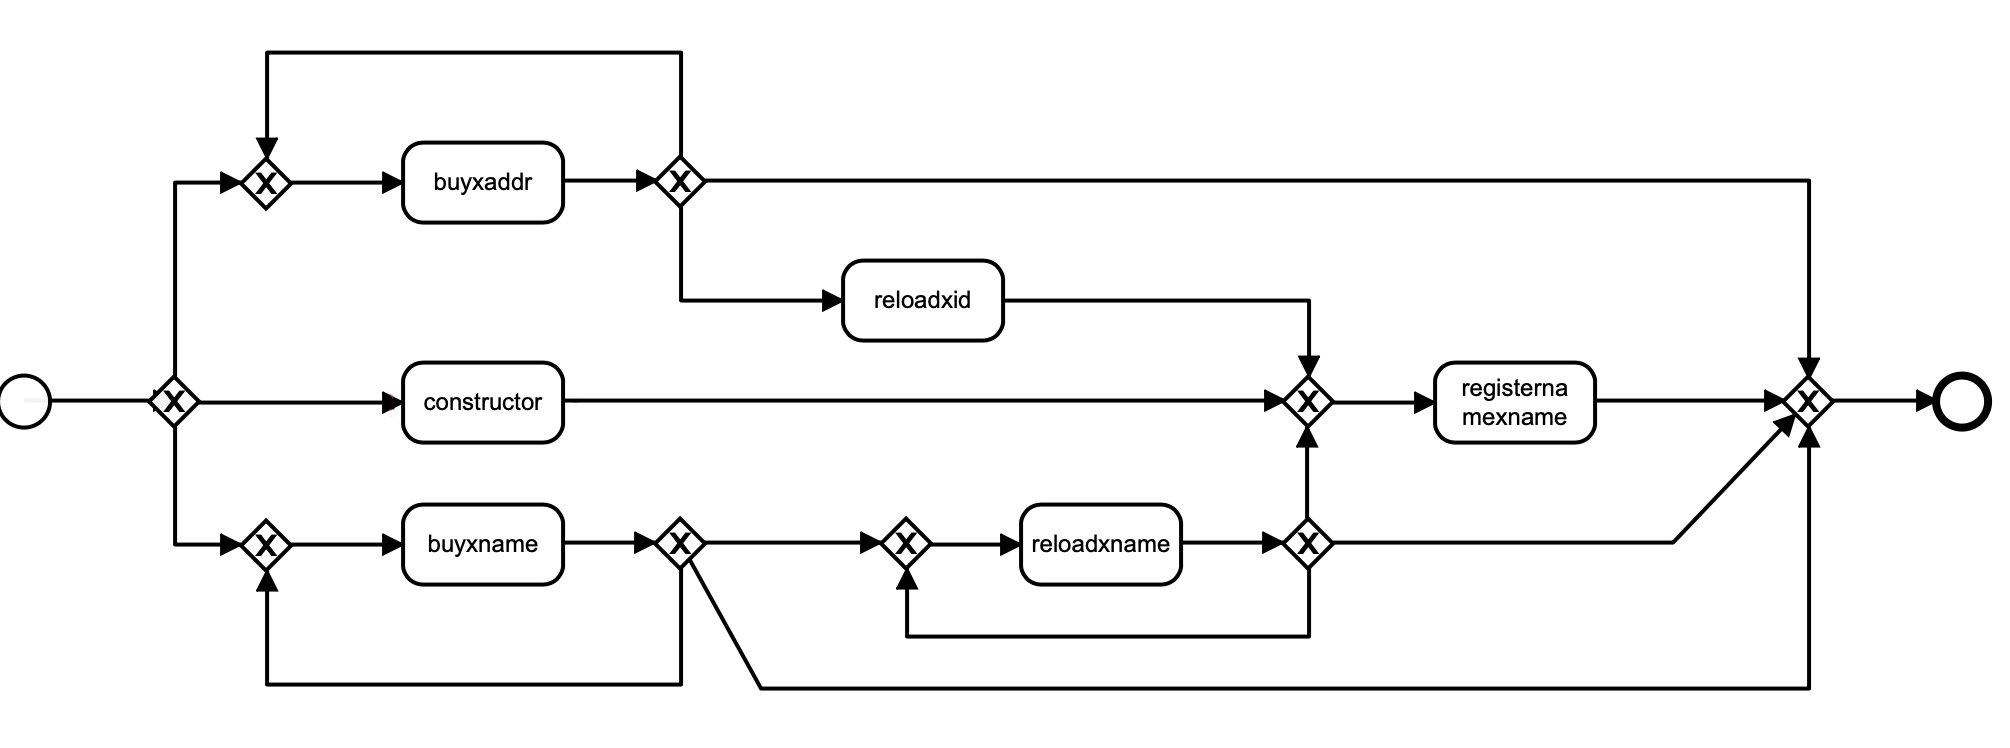
\includegraphics[width=1.2\textwidth]{images/fomo_inductive.png} }
    \caption{Fomo3D inductive miner}
    \label{images:fomo_inductive}
\end{figure}

\begin{figure}[!ht]
    \centering
    \makebox[\textwidth] { 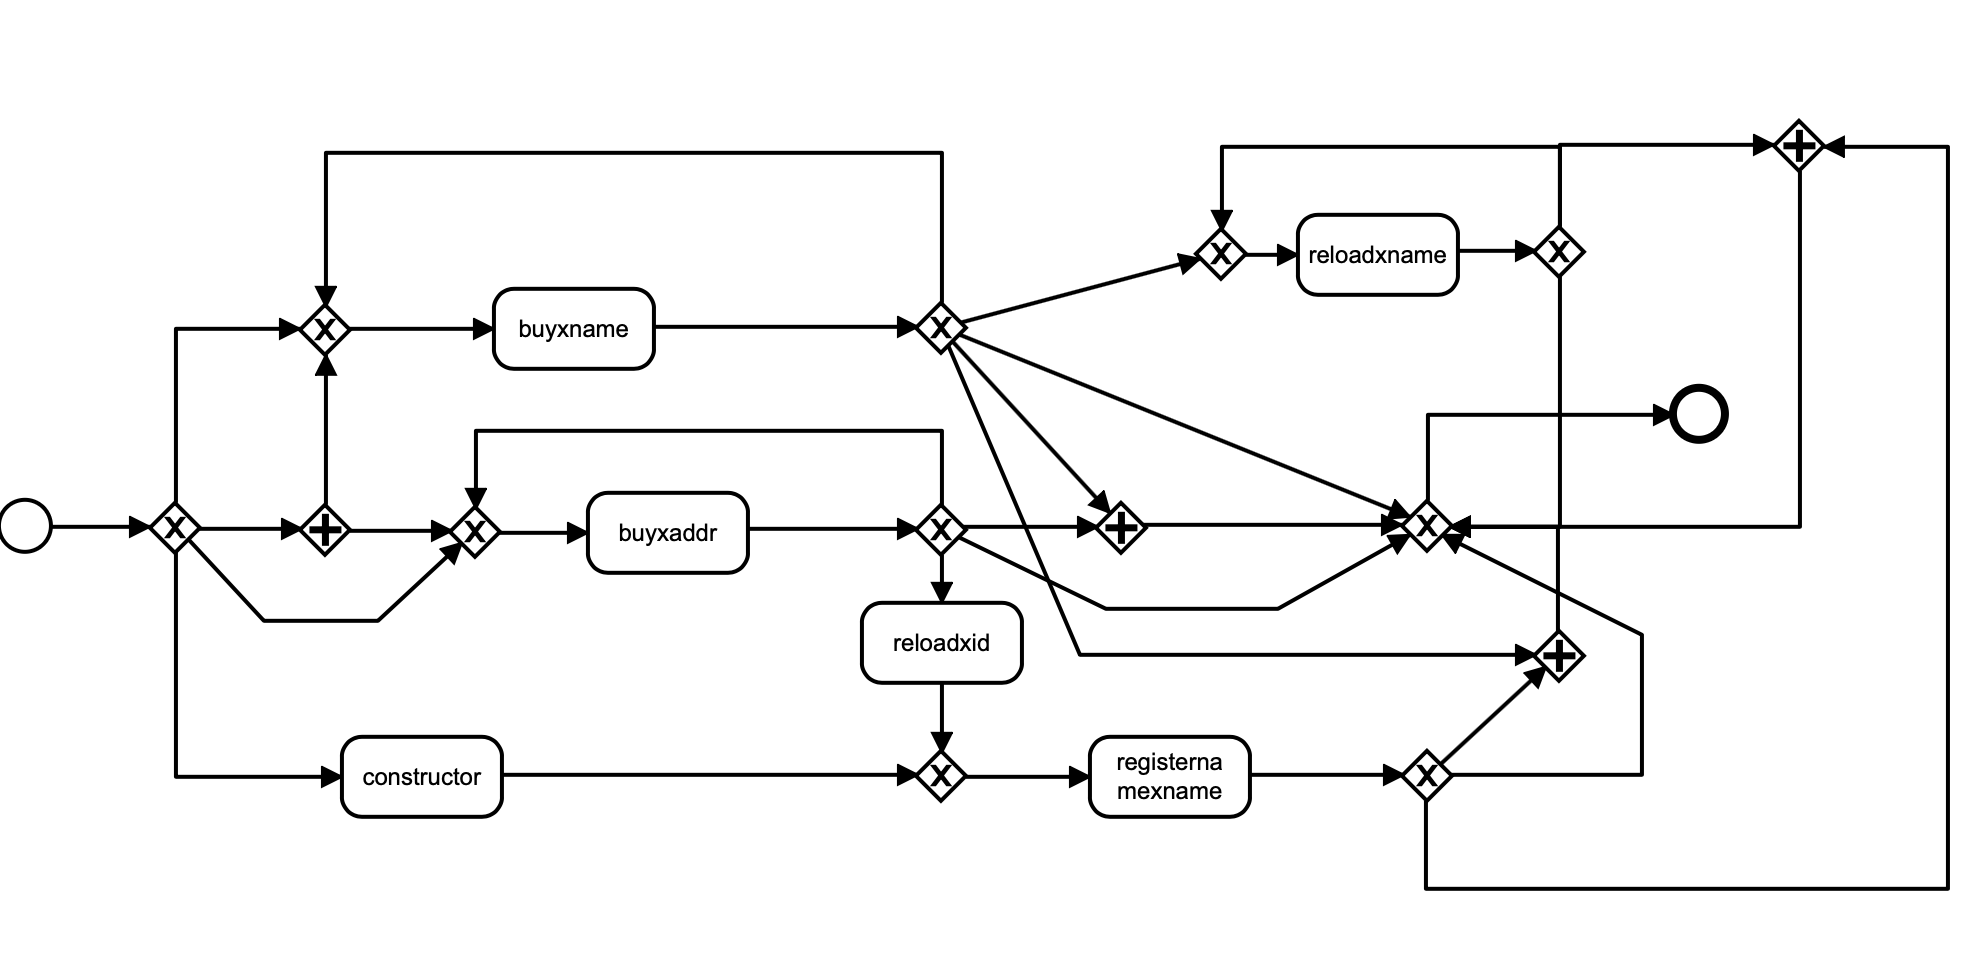
\includegraphics[width=1.2\textwidth]{images/fomo_heuristic.png} }
    \caption{Fomo3D heuristic miner}
    \label{images:fomo_heuristic}
\end{figure}

Both tasks ``buy*" and ``reload*" has a similar behaviour: they spends ETH to purchase keys in order to win the jackpot but with a 
small difference: ``buy*" use ETH from user wallet instead ``reload*" uses your unwithdrawn earnings. This is explained in a 
comment of the smart contract available on Ethereum.

In Table \ref{tables:fomo} the quality values measured:

\begin{center}
    \label{tables:fomo}
    \begin{tabular}{ | l | c | c | c | c |}
        \hline
        \textbf{Algorithm} & \textbf{BPMN to PN} & \textbf{Fitness} & \textbf{Precision} & \textbf{Generalization} \\ 
        \hline
        Split Miner & Ok & 0.97357 & 0.47947 & 0.96836 \\ 
        \hline
        Inductive Miner & Ok & 0.97357 & 0.47947 & 0.96836 \\
        \hline
        Heuristic Miner & Ok & 0.98710 & 0.48634 & 0.87593 \\
        \hline
    \end{tabular}
\end{center}

Even in this case fitness and generalization values are pretty high while precision is smaller even if more stable than the 
previous example. From the generalization point of view only heuristic miner has a bit smaller value. For Fomo3D both Split 
Miner and Inductive Miner discovered the same model and obviously also the quality measures are the same. Heuristic Miner 
this time inferred also the dirtier model. So in this case Split Miner and Inductive Miner perform better than Heuristic.


\section{IDEX}
\label{case_studies:idex}

Exchanges are applications that allows the user to deposit, withdraw or exchange cryptocurrencies: one of the most famous 
and used exchange running on Ethereum is IDEX (https://idex.market/eth/). IDEX is the first Ethereum based decentralized smart contract exchange to 
support real-time trading and high transaction throughput. IDEX is the most advanced Ethereum DEX, supporting limit and market 
orders, gas-free cancels, and the ability to fill many trades at once. IDEX allows users to trade all ERC20 tokens: ERC20 is 
an Ethereum standard that define the base behaviour of a token. On top of the standard, custom features can be added.
IDEX allow to buy/sell tokens using two approaches: 

\begin{itemize}
    \item \textbf{Limit order}, where the user define the amount of tokens to buy/sell, the token, and a limit: when the 
        value of the token reaches (increasing or decreasing) the limit defined the transaction will be commited to Ethereum. 
        Until that moment the transaction is in a pending state.
    \item \textbf{Market order}, in this case instead the transaction is commited immediatly using the current market value 
        of the token.
\end{itemize}

In this case the built log contains more than 2000 events grouped in 14 traces. Even in this case every user has a lot of interaction 
with the smart contract.

Figure \ref{images:idex_split} shows the model obtained applying the Split Miner algorithm, in Figure \ref{images:idex_inductive} 
is depicted the model inferred throug Inductive Miner and, finally Figure \ref{images:idex_heuristic} shows the result of the 
Heuristic Miner algorithm. 

\begin{figure}[!ht]
    \centering
    \makebox[\textwidth] { 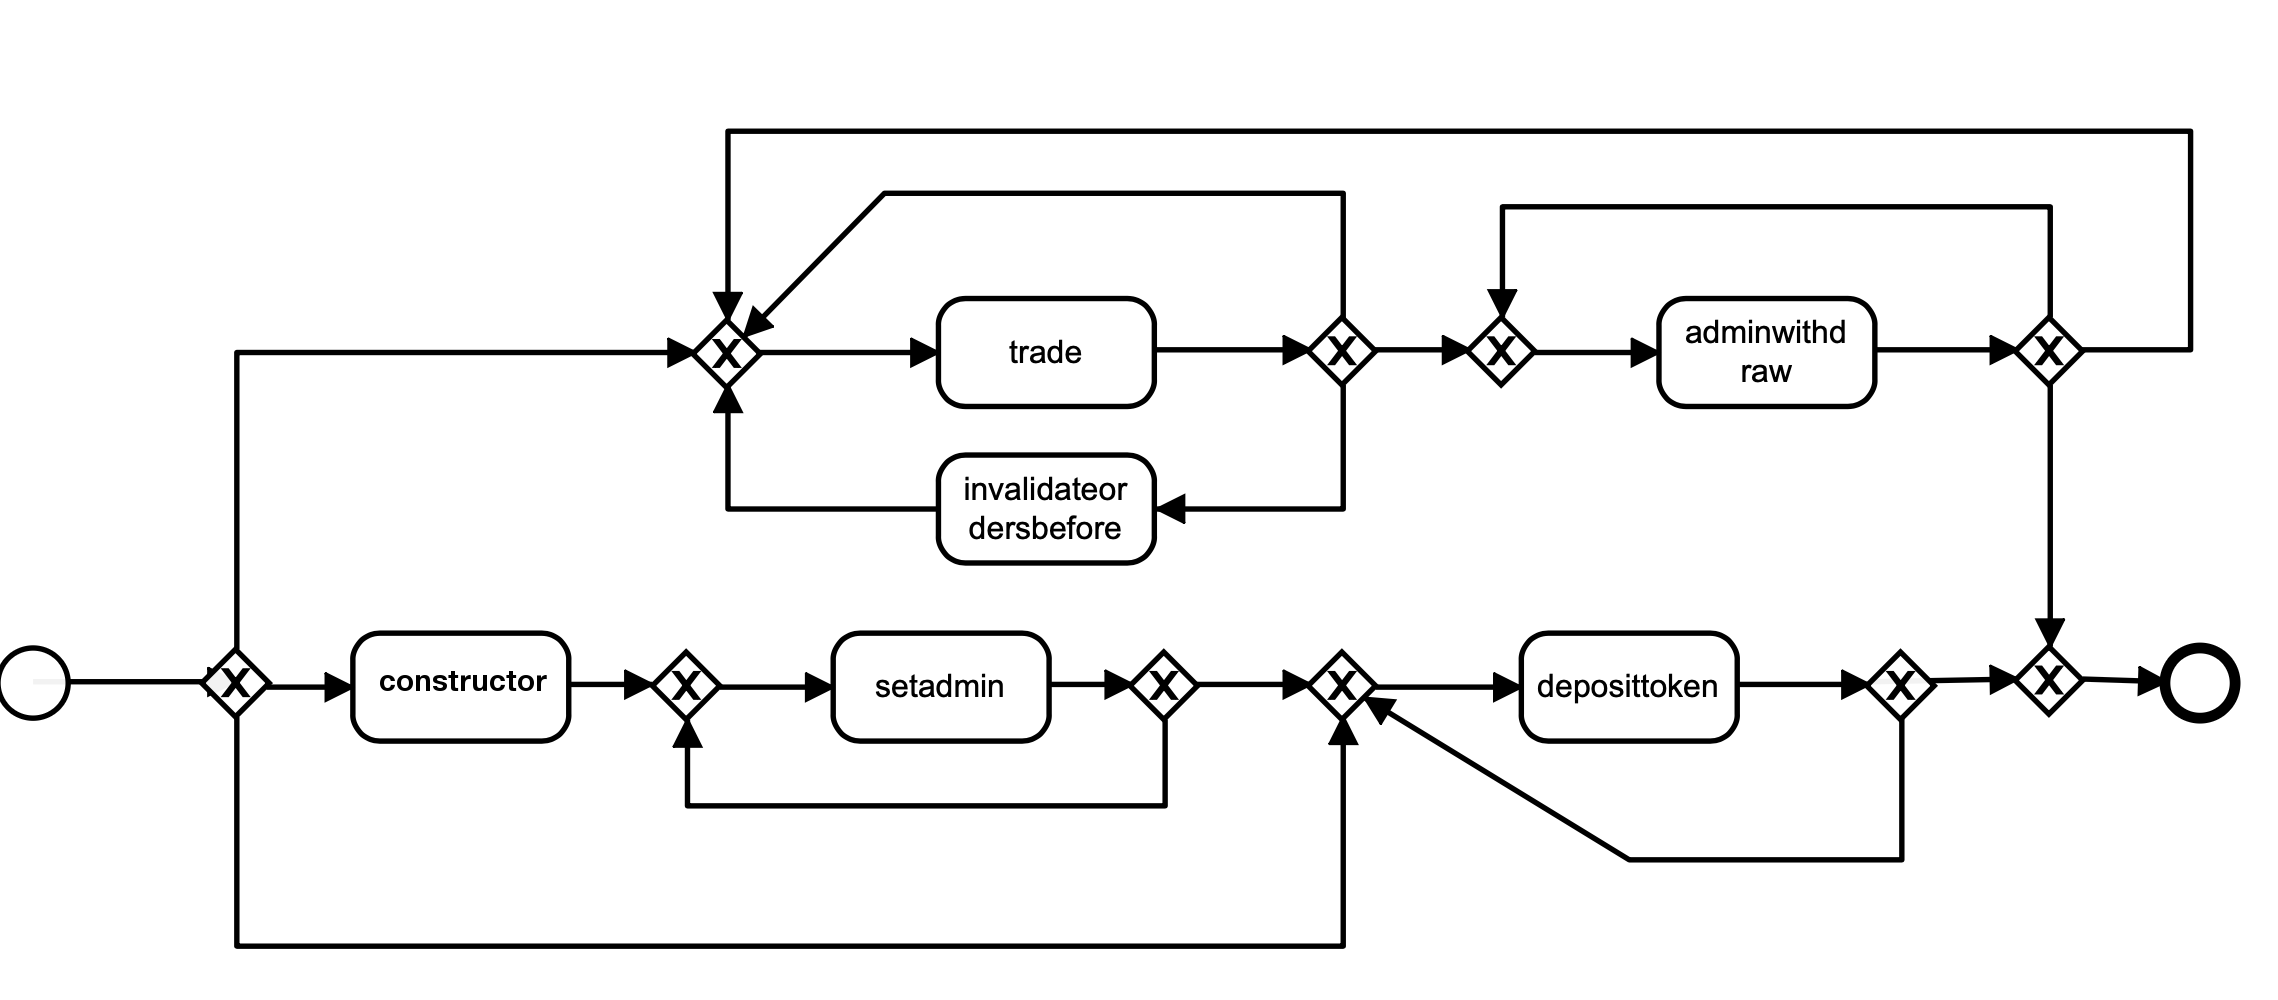
\includegraphics[width=1.2\textwidth]{images/idex_split.png} }
    \caption{IDEX split miner}
    \label{images:idex_split}
\end{figure}

\begin{figure}[!ht]
    \centering
    \makebox[\textwidth] { 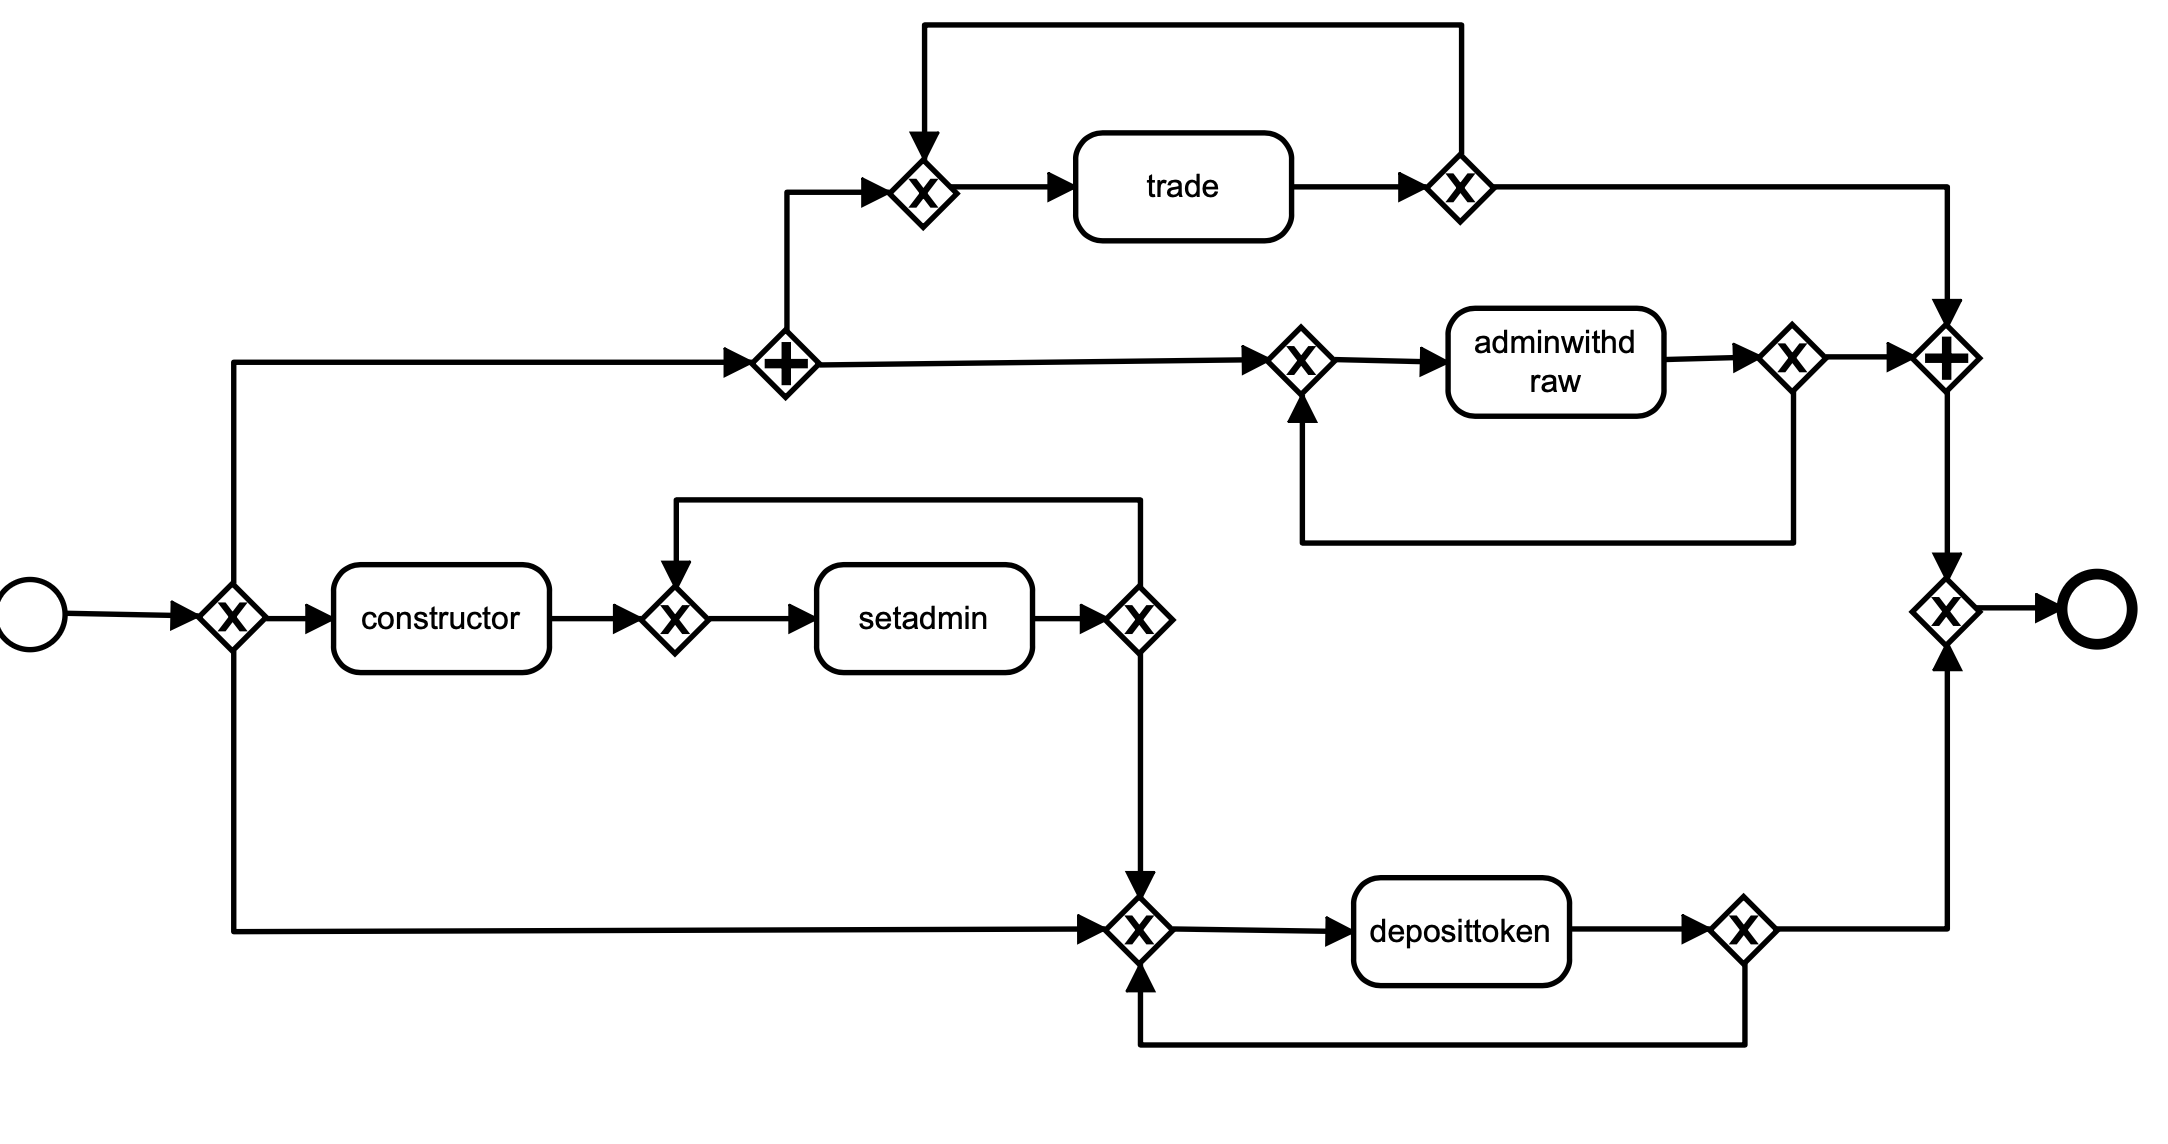
\includegraphics[width=1.2\textwidth]{images/idex_inductive.png} }
    \caption{IDEX inductive miner}
    \label{images:idex_inductive}
\end{figure}

\begin{figure}[!ht]
    \centering
    \makebox[\textwidth] { 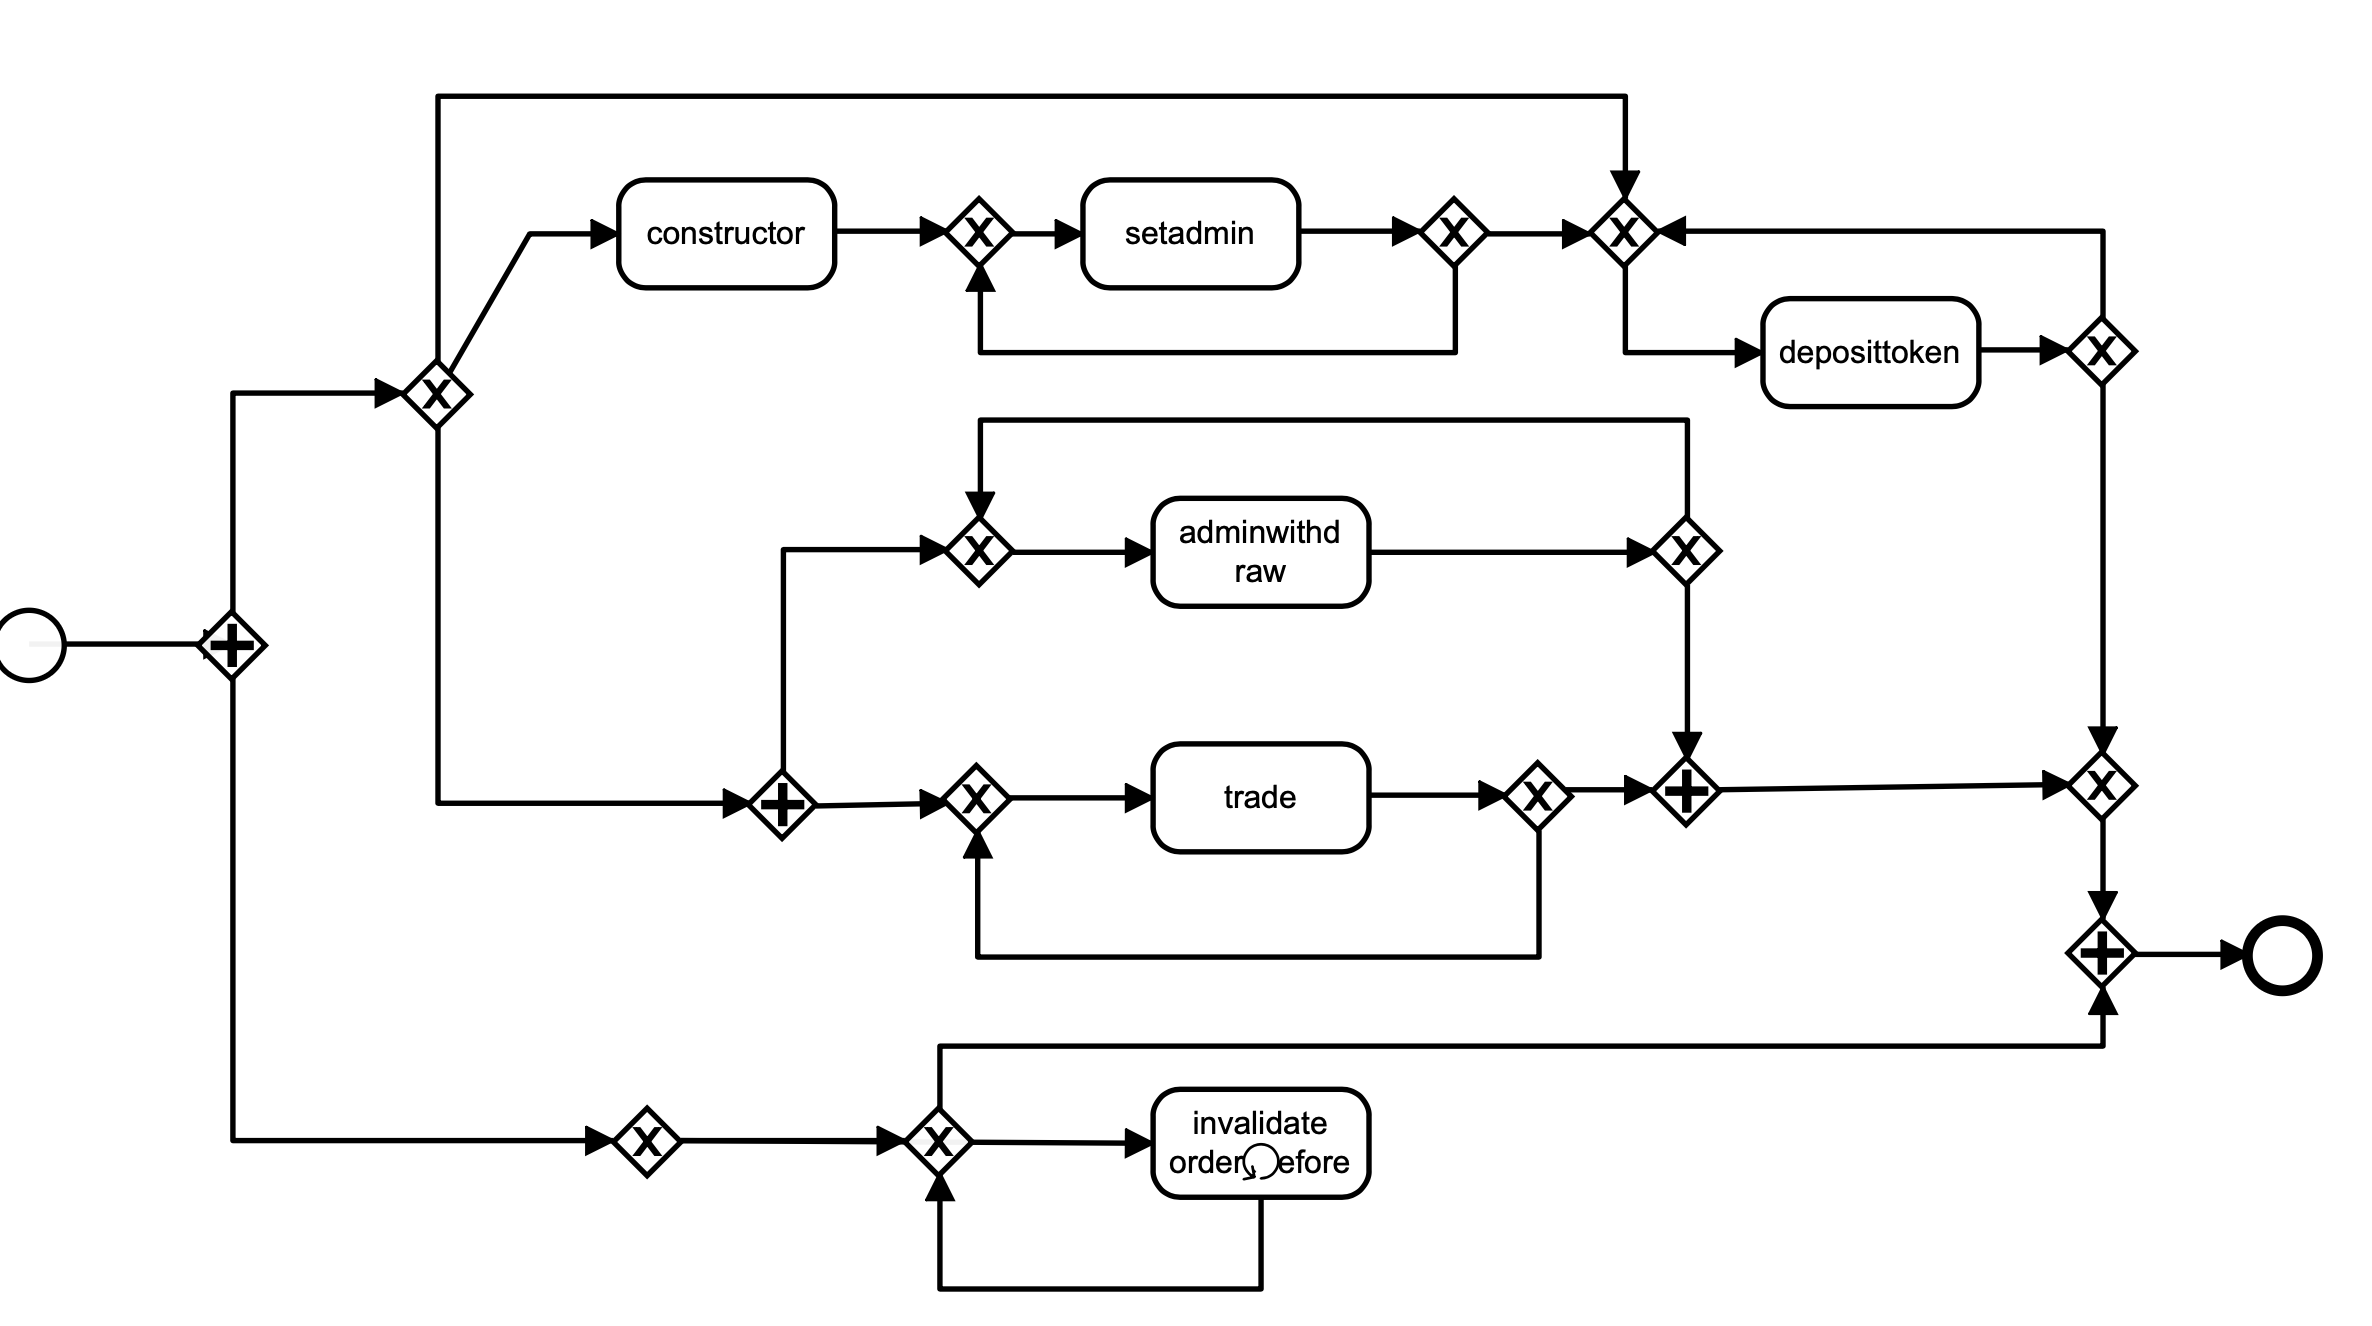
\includegraphics[width=1.2\textwidth]{images/idex_heuristic.png} }
    \caption{IDEX heuristic miner}
    \label{images:idex_heuristic}
\end{figure}

Table \ref{table:idex_results} shows the quality values measured:

\begin{center}
    \begin{tabular}{ | l | c | c | c | c |}
        \hline
        \textbf{Algorithm} & \textbf{BPMN to PN} & \textbf{Fitness} & \textbf{Precision} & \textbf{Generalization} \\ 
        \hline
        Split Miner & Ok & 0.99573 & 0.22884 & 0.99914 \\ 
        \hline
        Inductive Miner & Ok & 0.99971 & 0.48298 & 0.99968 \\
        \hline
        Heuristic Miner & Ok & 1 & 0.32516 & 0.99882 \\
        \hline
    \end{tabular}
    \label{table:idex_results}
\end{center}

As in the previous cases Fitness and Generalization are stable and high, instead Precision is less stable and not so high.
This time analysing the models the Inductive Miner skipped a task (it was filtered out) but despite this it performed 
better than the others in the quality measures expecially for the Precision. From the point of view of models readability all 
the three algorithms performed well in this case study.


\section{Lessons learned}
The used approach has allowed to obtain good results with sound models discovered and pretty good quality parameters 
measured. Even if the process is a bit articulated and mechanical the used tools were simple to use, reliable and 
they work well together.
In the construction phase of the log the choice to group the transitions for smart contracts has been a winning one 
because it has highlighted a link between the different transitions. One aspect that could be improved during the building of 
the log is to take in consideration the time variable during the grouping of the activities in traces: an idea can be to do 
some clustering defining the time interval of a trace.

The analysis of how and how many transitions use a smart contract results in deducing the logic with which these transitions 
were generated, ie the logic of the DAPPs. This analysis can be seen as a kind of reverse engeenering. 

The three different algorithms used have obtained very similar results and in every case study a different algorithm performed 
better than the others. In general these observations let think that the measure of how well an algorithm fits a specific 
application domain depends from the business logic of this domain regardless the fact that it uses the Blockchain.

Potentially the methodology used in this chapter, adequately refined, could also be used to understand how a user interacts with 
a system and compares different behaviors. Going even further in this direction we could understand the tastes and 
characteristics of certain users by analyzing how they interacted on different systems.
\chapter{Design and implementation}
\label{design_implementation}

This chapter aims to tell the process of design and implementation of a Mining Framework. This system helps its users to 
recreate the steps done in the case studies analysis in previous chapter using a single UI. Its main goal is to automize the 
mining activity and gain a deeper control on the overall process.

This chapter is composed from section \ref{desing:overview} where the mining framework is introduced and from section 
\ref{desing:architecture} where the solution is described in detail starting from two images that depict the achitecture of the 
system and how messages are exchanged between software components. After that, these images are described in detail.


\section{Solution overview}
\label{desing:overview}
The developed Mining framework want to allow its users to extract information from the blockchain using process mining techniques 
even if they are not experts. In fact it emulates the steps applied in chapter \ref{case_studies} but hiding some complexities to 
the user: for example it is not more needed to know Disco, ProM and Apromore and how to use them. All the process is automated 
and can be started with few clicks. 

The solution is structured in two applications: a front-end and a back-end. The front-end is developed in Angular because of its 
simplicity, the great support over it and its good performances. The UI is designed for simplicity and is based on Google Material 
Design. The server is developed in java because of the need to integrate some ProM libraries for the mining algorithms 
implementation.


\section{Solution architecture}
\label{desing:architecture}

Figure \ref{images:desing_architecture} shows the architecture of the system in a component diagram.

\begin{figure}[!ht]
    \centering
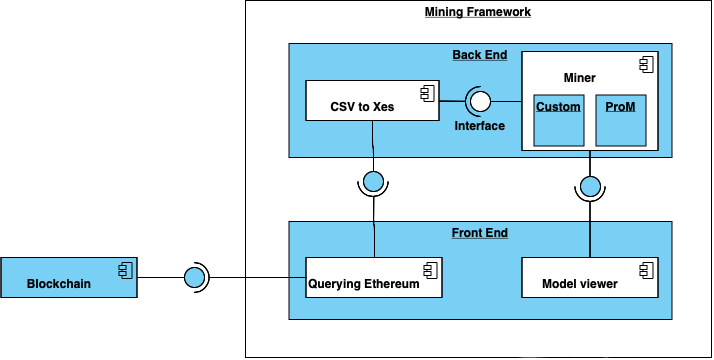
\includegraphics[width=\textwidth]{images/component_diagram.png}
    \caption{Solution architecture}
    \label{images:desing_architecture}
\end{figure}

In this diagram there are the Mining Framework and the blockchain that are two separate and independent systems which interact 
each other. Ethereum is the blockchain component for this thesis. Instead the the Mining Framework is a software solution 
composed by four main components arranged in a front-end and a back-end. These components are:

\begin{itemize}
    \item \textbf{Querying}, this component has the goal to extract data from the blockchain. It is part of the front-end 
        application so it is implemented in Angular. In order to 
        interact with the blockchain it uses Web3.js that, being a javascript library is compatible with Typescript, the 
        programming language used in Angular development. The development of this component has been inspired by the SQL 
        language: this language is used to extract integrated data from databases. In general SQL has a lot of features but only 
        a subset of them are needed in the Querying component: for example indexing, editing and creations are unusefull for the purpose of 
        the thesis. For this the "Querying component" is built as a graphical query language: it leads the user in the building of the 
        query, reducing the error probability. It has a simple and effective UI in order to make easy for users to create their queries.
        In figure \ref{images:design_query_screen} there is a screenshot taken to the application while building a query (in this
        case the query filters for all the transactions with a value grater than two and then select only few properties from the 
        filtered transactions set).

        \begin{figure}[!ht]
            \centering
        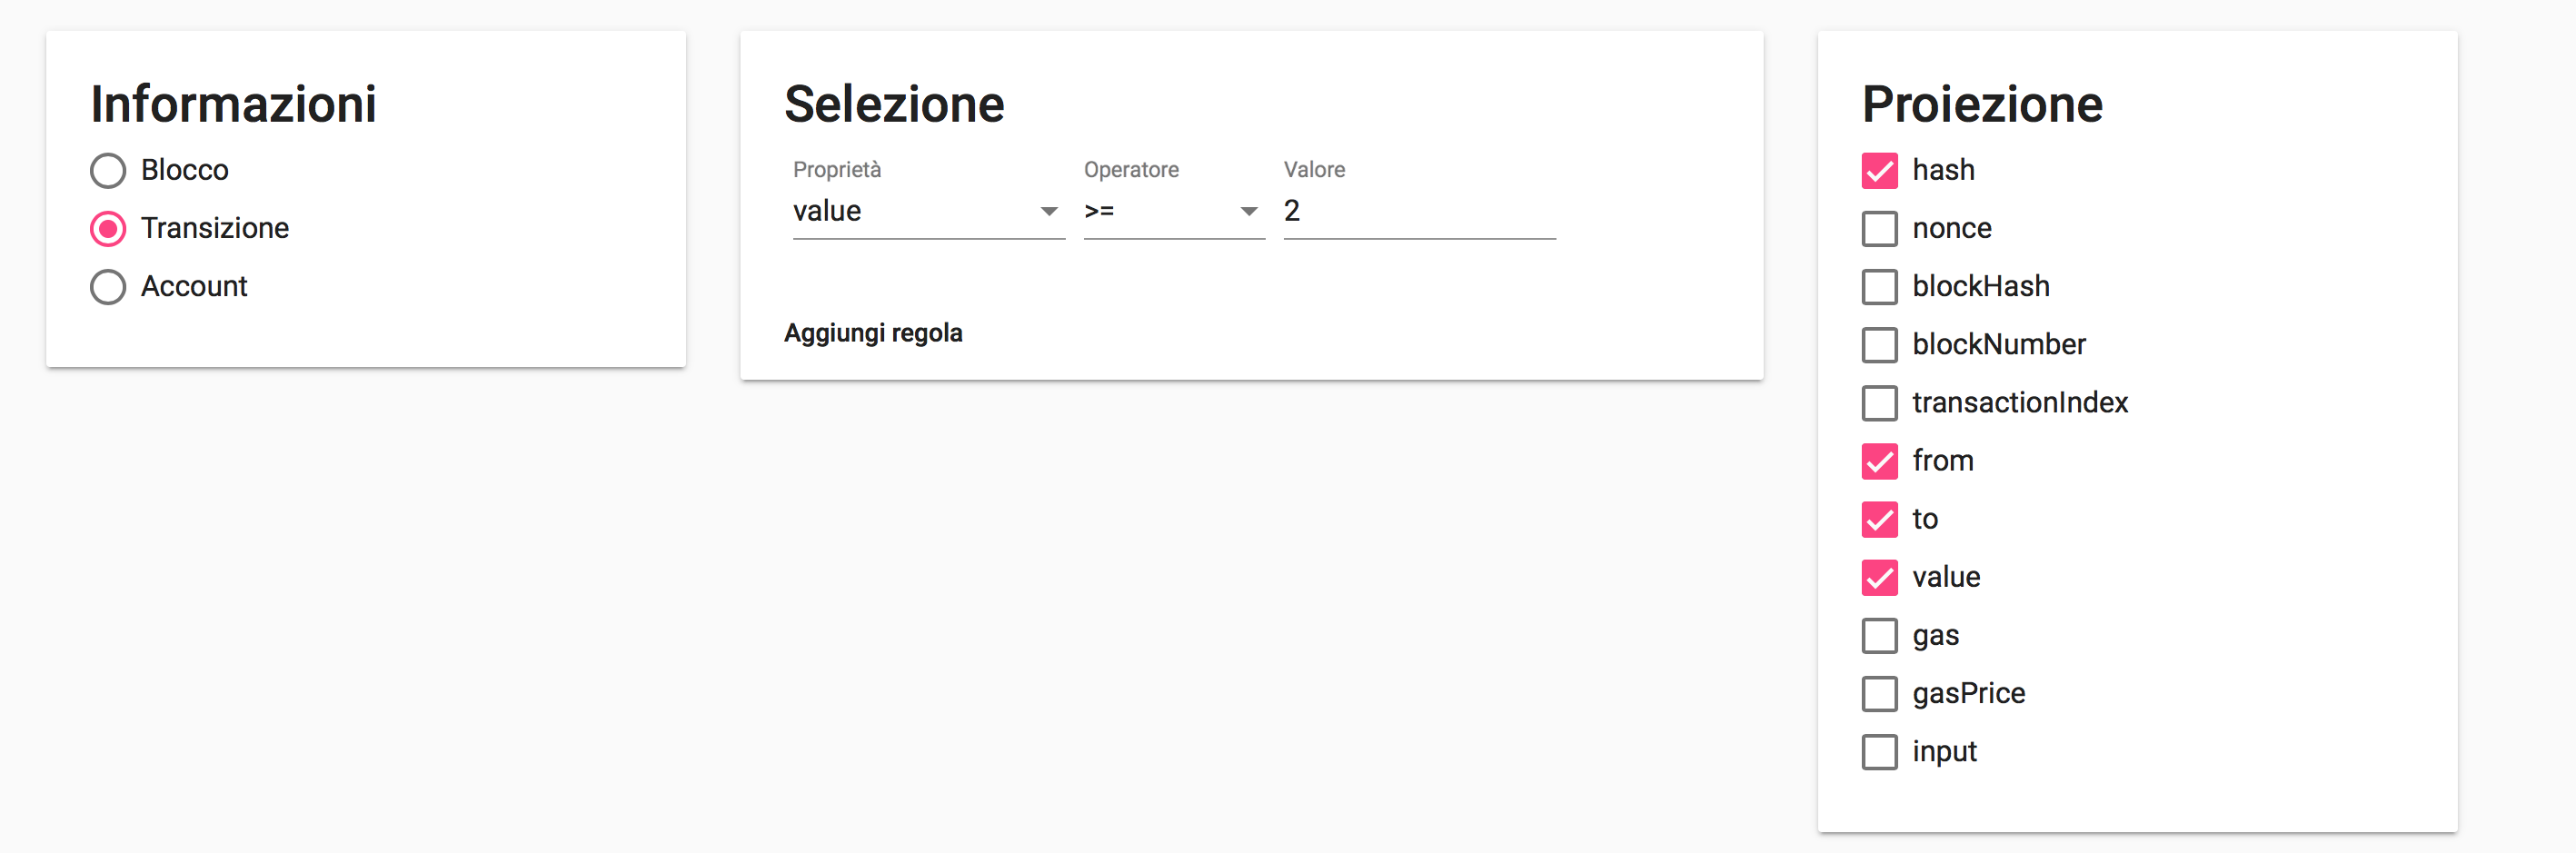
\includegraphics[width=\textwidth]{images/design_query_screen.png}
            \caption{Example of query}
            \label{images:design_query_screen}
        \end{figure}

        The application allow the user to build also complex queries using logical operators to join different simpler expressions.
        During the development some limitations, caused by the nature of the Blockchain, emerged: there are not calls that allow 
        to recover aggregated data, but only single elements are served: this means that when working with huge numbers of entities 
        the performance are really poor (every call to Web3.js api consist of a RPC call). This problem can be solved only 
        reproducing the work done by Etherscan: substantially syncing with Ethereum and creating a local db with indexes that 
        allow for fast access to all stored data. For the thesis purpose the performances are not so important so another solution 
        was adopted: partial results are shown live during the query execution. This feature does not reduce the total amount of 
        time needed to execute the query but at least gives the user a feedback about what is happening, making the application 
        usable.
        Querying allows to export query results in csv or json format.
    
    \item \textbf{CSV to Xes}, this component transform a CSV file in a Xes file. Generally it receive the results of a query 
        done with the Querying component and then produce a Xes file ready to be analyzed. This transformaion is done in the back-end 
        application beacuse here is possible to use ProM Java libraries that help in this convertion procedure.

    \item \textbf{Miner}, this component is the one responsible of the inference procedure and it is part of the back-end 
        application. It receives a Xes file and produces a model represented as Petri Net. Actually the discovery activity is based on 
        the Inductive Miner algorithm: more precisely, on the ProM implementation of the Inductive Miner. Despite this it has a 
        modular structure and more algorithms, custom or from ProM, can be easily added.

    \item \textbf{Model Viewer}, this is the component responsible for the representation of the results obtained in the mining 
        process. It receives the Petri Net infered and show it to the user.

\end{itemize}

After the presentation of the system components in Figure \ref{images:sequence_flow} is depicted a sequence diagram that 
describes the message flow between software components.

\begin{figure}[!ht]
    \centering
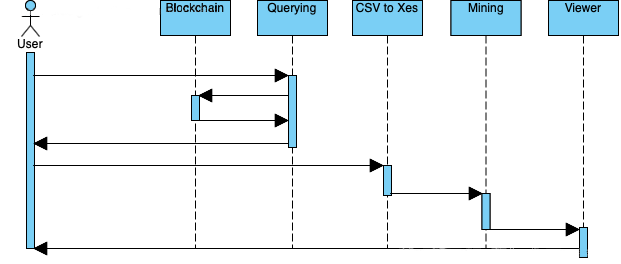
\includegraphics[width=\textwidth]{images/sequence_diagram.png}
    \caption{Message flow between system components}
    \label{images:sequence_flow}
\end{figure}

The overall process is started by the user that interacts with the Querying component: he create the query and execute it. After 
that the Querying component returns the results to the user who can choose if export these results or to use them to start a 
Mining process. In this second case data are sent to the server in CSV format: the back-end uses the converter component in order 
to obtain a Xes file that is sent to the Miner. The Miner apply the Inductive Miner algorithm and generates a Petri Net from the 
Xes file, after that it sends the Petri Net back to the client where the Model Viewer shows it.
\chapter{Conclusions and future works}

In general the importance of process mining for industries is known because  it allow to reduce costs, optimize resource 
handling and how the work is done. Over that it also allows to assist the live execution of the process with predictions 
(as for example completation time or the next choice).

Blockchain has a huge potential and it can change a lot of business areas despite it is still a quite immature technology. 
In last times great investments has been made on this technology even from huge companies  and this means that its 
development will be really fast in next years.

The work done in this thesis shows that is possible, combining the processing power of process mining and the execution power 
of the blockchain, to infer the logic behind systems that uses Ethereum as decentralized server. This consideration can have a 
lot of future developments: for example companies can provide a validity check service for applications resident on the 
blockchain. The blockchain transparency itself can be enhanced by the combination of these two technologies because people or 
organizations external to the application domain can check the correctness of the behaviour of the system. Also the same 
developers can use these techniques to test their applications. Another interesting use case could be the extraction of the 
system structure in order to express it in a format understandable from company managers even if they have not technical 
competence. Obviously all this transparency can also be seen from a negative point of view: if a company has built its 
competitive advantage towards competitors thanks to advanced business logic the possibility that someone else can deduce this 
logic and reduce the market gap is certainly a negative aspect that can lead companies to be wary of this type of technologies.

With the design and implementation part, a prototype of a tool was created that allows the user in a few steps to perform 
analysis on the blockchain. There are many possible future developments such as the addition of new algorithms, the export 
from the server of an already rendered image of the petri net, the export from Querying Ethereum directly to XES, etc.

\bibliographystyle{plainnat}
\bibliography{bibliography}

\end{document}
